\section{Tables}
\label{app:ShapeFunctionTable}

\subsection{Polynomials}

%%%%%%%%%%%%%%%%%%%%%Polynomials 1: Legendre%%%%%%%%%%%%%%%%%%%%%
\renewcommand{\arraystretch}{1.35}%Better row spacing
\begin{center}
\begin{tabular}
{|C{0.35cm} L{11.9cm} C{2.9cm}|N}%See main file for this custom columns - they keep a fixed width while maintaining aligment
\hline
\multicolumn{3}{|c|}{\large \textbf{Polynomials}} &\\
\hline
\multicolumn{3}{|c|}{Legendre} &\\
\hline
{}& {} &{} &\\[-23pt]%To keep total width fixed
\multicolumn{3}{|l|}{Shifted and scaled Legendre polynomials for $t\geq0$ and $x\in[0,t]$:} &\\
\multicolumn{3}{|l|}{
$\begin{aligned}
	P_0(x;t)&=1\\
	P_1(x;t)&=2x-t\\
	iP_i(x;t)&=(2i-1)(2x-t)P_{i-1}(x;t)-(i-1)t^2P_{i-2}(x;t) \quad \text{for }\, i\geq2
\end{aligned}$} &\\
\multicolumn{3}{|l|}{Integrated Legendre polynomials:} &\\
\multicolumn{3}{|l|}{
$	\begin{aligned}
		2(2i-1)L_i(x; t)&=P_i(x;t)-t^2P_{i-2}(x;t) \quad\text{for }\, i\geq2
	\end{aligned}$} &\\
\multicolumn{3}{|l|}{Scaling differential of integrated Legendre polynomials:} &\\
\multicolumn{3}{|l|}{
$	\begin{aligned}
		\textstyle{\frac{\partial}{\partial t}}L_{i+1}(x;t)
			&=R_i(x;t)=-\textstyle{\frac{1}{2}}(P_i(x;t)+tP_{i-1}(x;t))\quad\text{for }\,i\geq1
	\end{aligned}$} &\\
\multicolumn{3}{|l|}{Homogenized polynomials:} &\\
\multicolumn{3}{|l|}{
$	\begin{aligned}{}
		[P_i](s_0,s_1)&=P_i(s_1;s_0+s_1)\quad\text{for }\, i\geq0\\
		[R_i](s_0,s_1)&=R_i(s_1;s_0+s_1)\quad\text{for }\, i\geq1\\
		[L_i](s_0,s_1)&=L_i(s_1;s_0+s_1)\quad\text{for }\, i\geq2\\
		\nabla[L_i](s_0,s_1)&=[P_{i-1}](s_0,s_1)\nabla s_1+[R_{i-1}](s_0,s_1)\nabla(s_0+s_1)
			\quad\text{for }\, i\geq2
	\end{aligned}$} &\\	
\multicolumn{3}{|l|}{$\,\,$ where $s_0$ and $s_1$ are functions of some spatial variable in $\R^N$, so $\nabla s_0,\nabla s_1\in\R^N$, for $N=1,2,3$.} &\\[-17pt]
{}& {} &{} &\\[-5pt]
\multicolumn{3}{r}{\footnotesize\textit{continued on next page}} &\\[-18.5pt]
\hline
\end{tabular}
\end{center}
\renewcommand{\arraystretch}{1}%Back to normal spacing

\newpage

%%%%%%%%%%%%%%%%%%%%%Polynomials 2: Jacobi%%%%%%%%%%%%%%%%%%%%%
\renewcommand{\arraystretch}{1.35}%Better row spacing
\begin{center}
\begin{tabular}
{|C{0.35cm} L{11.9cm} C{2.9cm}|N}%See main file for this custom columns - they keep a fixed width while maintaining aligment
\multicolumn{3}{l}{\footnotesize\textit{continued from previous page}} &\\[-2pt]
\hline
\multicolumn{3}{|c|}{\large \textbf{Polynomials}} &\\
\hline
\multicolumn{3}{|c|}{Jacobi} &\\
\hline
{}& {} &{} &\\[-23pt]%To keep total width fixed
\multicolumn{3}{|l|}{Shifted and scaled Jacobi polynomials for $\alpha>-1$, $t\geq0$ and $x\in[0,t]$:} &\\
\multicolumn{3}{|l|}{
$	\begin{aligned}
		P_0^\alpha(x;t) &= 1 \\
		P_1^\alpha(x;t) &= 2x-t+\alpha x\\
		a_j{P}_j^\alpha(x;t)&=b_j(c_j(2x-t)+\alpha^2 t)P_{j-1}^\alpha(x;t)-d_jt^2 P_{j-2}^\alpha(x;t)
		\quad \text{for }\, j\geq2
	\end{aligned}$} &\\
\multicolumn{3}{|l|}{$\,\,$ where} &\\
\multicolumn{3}{|l|}{
$	\begin{aligned}{}
		\qquad a_j &=  2j(j+\alpha)\, (2j + \alpha - 2)\\
		\qquad b_j &=  2j + \alpha - 1\\
		\qquad c_j &=  (2j+\alpha)\, (2j + \alpha - 2)\\
		\qquad d_j &=  2(j+\alpha-1)\, (j-1)\, (2j+\alpha)
	\end{aligned}$} &\\
\multicolumn{3}{|l|}{Integrated Jacobi polynomials:} &\\
\multicolumn{3}{|l|}{
$	\begin{aligned}
		L^{\alpha}_1(x;t)&= x\\
		L^{\alpha}_j(x;t)&=a_j P^{\alpha}_j(x,t)+b_jtP^{\alpha}_{j-1}(x;t)-c_jt^2P^{\alpha}_{j-2}(x;t)
			\quad\text{for }\, j\geq2
	\end{aligned}$} &\\
\multicolumn{3}{|l|}{$\,\,$ where} &\\
\multicolumn{3}{|l|}{
$	\begin{aligned}{}
		\qquad a_j = & \textstyle{\frac{j + \alpha}{(2j + \alpha -1)(2j + \alpha)}} \\
		\qquad b_j = & \textstyle{\frac{\alpha}{(2j + \alpha -2)(2j + \alpha)}} \\
		\qquad c_j = & \textstyle{\frac{j-1}{(2j + \alpha -2)(2j + \alpha-1)}}
	\end{aligned}$} &\\
\multicolumn{3}{|l|}{Scaling differential of integrated Jacobi polynomials:} &\\
\multicolumn{3}{|l|}{
$	\begin{aligned}
		\textstyle{\frac{\partial}{\partial t}}L_1^\alpha(x;t)&=R_0^\alpha(x;t)=0\\
		\textstyle{\frac{\partial}{\partial t}}L_{j+1}(x;t)
			&=R^\alpha_j(x;t) = -\textstyle{\frac{j}{2j+\alpha}}(P^\alpha_j(x;t)+tP^\alpha_{j-1}(x;t))
				\quad\text{for }\,j\geq1
	\end{aligned}$} &\\
\multicolumn{3}{|l|}{Homogenized polynomials:} &\\
\multicolumn{3}{|l|}{
$	\begin{aligned}{}
		[P_j^\alpha](t_0,t_1)&=P_j^\alpha(t_1;t_0+t_1)\quad\text{for }\, j\geq0\\
		[R_j^\alpha](t_0,t_1)&=R_j^\alpha(t_1;t_0+t_1)\quad\text{for }\, j\geq0\\
		[L_j^\alpha](t_0,t_1)&=L_j^\alpha(t_1;t_0+t_1)\quad\text{for }\, j\geq1\\
		\nabla[L_j^\alpha](t_0,t_1)&=[P_{j-1}^\alpha](t_0,t_1)\nabla t_1+[R_{j-1}^\alpha](t_0,t_1)\nabla(t_0+t_1)
			\quad\text{for }\, j\geq1
	\end{aligned}$} &\\	
\multicolumn{3}{|l|}{$\,\,$ where $t_0$ and $t_1$ are functions of some spatial variable in $\R^N$, so $\nabla t_0,\nabla t_1\in\R^N$, for $N=1,2,3$.} &\\[-17pt]
{}& {} &{} &\\
\hline
\end{tabular}
\end{center}
\renewcommand{\arraystretch}{1}%Back to normal spacing

\newpage
\subsection{Ancillary Operators}

%%%%%%%%%%%%%%%%%%%%%Ancillary 1: H1 and Hcurl%%%%%%%%%%%%%%%%%%%%%
\renewcommand{\arraystretch}{1.35}%Better row spacing
\begin{center}
\begin{tabular}
{|C{0.35cm} L{11.9cm}|C{2.9cm}|N}%See main file for this custom columns - they keep a fixed width while maintaining aligment
\hline
\multicolumn{3}{|c|}{\large \textbf{Ancillary Operators}} &\\
\hline
\multicolumn{3}{|c|}{\small In all cases, $s_0$, $s_1$, $s_2$, $t_0$ and $t_1$ are functions of some spatial variable in $\R^N$.} &\\
\hline
\multicolumn{3}{|c|}{$H^1$} &\\
\hline
{}& {} &{} &\\[-23pt]%To keep total width fixed
\multicolumn{2}{|c|}{Operator}& Indices &\\ \hline
\multicolumn{2}{|l|}{Edge} &
\multirow{2}{*}[-12pt]{\small$\begin{gathered}
N\!=\!1,2,3\\
i\!=\!2,\ldots,p_s
\end{gathered}$} &\\
\multicolumn{2}{|l|}{
$	\begin{aligned}
		\phi^\E_i(s_0,s_1)&=[L_i](s_0,s_1)\\
		\nabla\phi^\E_i(s_0,s_1)&=\nabla[L_i](s_0,s_1)
	\end{aligned}$} &{}&\\
\multicolumn{2}{|l|}{Quadrilateral Face} &
\multirow{2}{*}[-5pt]{\small$\begin{gathered}
N\!=\!2,3\\
i\!=\!2,\ldots,p_s\\
j\!=\!2,\ldots,p_t
\end{gathered}$} &\\
\multicolumn{2}{|l|}{
$	\begin{aligned}
		\phi_{ij}^\square(s_0,s_1,t_0,t_1)&=\phi_i^\E(s_0,s_1)\phi_j^\E(t_0,t_1)\\
		\nabla\phi_{ij}^\square(s_0,s_1,t_0,t_1)&=\phi_i^\E(s_0,s_1)\nabla\phi_j^\E(t_0,t_1)+\phi_j^\E(t_0,t_1)\nabla\phi_i^\E(s_0,s_1)
	\end{aligned}$} &{}&\\
\multicolumn{2}{|l|}{Triangle Face} &
\multirow{2}{*}[-5pt]{\small$\begin{gathered}
N\!=\!2,3\\
i\geq2,\,j\geq1\\
i\!+\!j\!=\!3,\ldots,p_s
\end{gathered}$} &\\
\multicolumn{2}{|l|}{
$	\begin{aligned}
		\phi_{ij}^\Tri(s_0,s_1,s_2)&=\phi_i^\E(s_0,s_1)[L_j^{2i}](s_0+s_1,s_2)\\
		\nabla\phi_{ij}^\Tri(s_0,s_1,s_2)&=[L_j^{2i}](s_0\!+\!s_1,s_2)\nabla\phi_i^\E(s_0,s_1)
			+\phi_i^\E(s_0,s_1)\nabla[L_j^{2i}](s_0\!+\!s_1,s_2)
	\end{aligned}$} &{}&\\[-17pt]
{}& {} &{} &\\
\hline
\multicolumn{3}{|c|}{$H(\mathrm{curl})^\star$} &\\
\hline
{}& {} &{} &\\[-23pt]%To keep total width fixed
\multicolumn{2}{|c|}{Operator}& Indices &\\ \hline
\multicolumn{2}{|l|}{Edge$^\diamond$} &
\multirow{2}{*}[-12pt]{\small$\begin{gathered}
N\!=\!2,3\\
i\!=\!0,\ldots,p_s\!-\!1
\end{gathered}$} &\\
\multicolumn{2}{|l|}{
$	\begin{aligned}
		E^\E_i(s_0,s_1)&=[P_i](s_0,s_1)(s_0\nabla s_1-s_1\nabla s_0)\\
		\nabla\!\times\! E_i^\E(s_0,s_1)&=(i+2)[P_i](s_0,s_1)\nabla s_0\!\times\!\nabla s_1
	\end{aligned}$} &{}&\\
\multicolumn{2}{|l|}{Quadrilateral Face} &
\multirow{2}{*}[-5pt]{\small$\begin{gathered}
N\!=\!2,3\\
i\!=\!0,\ldots,p_s\!-\!1\\
j\!=\!2,\ldots,p_t
\end{gathered}$} &\\
\multicolumn{2}{|l|}{
$	\begin{aligned}
		E_{ij}^{\square}(s_0,s_1,t_0,t_1)&=\phi_j^\E(t_0,t_1)E_i^\E(s_0,s_1)\\
		\nabla\!\times\! E_{ij}^{\square}(s_0,s_1,t_0,t_1)&=\phi_j^\E(t_0,t_1)\nabla\!\times\! E_i^\E(s_0,s_1)
    	+\nabla\phi_j^\E(t_0,t_1)\!\times\! E_i^\E(s_0,s_1)
	\end{aligned}$} &{}&\\
\multicolumn{2}{|l|}{Triangle Face} &
\multirow{2}{*}[-12pt]{\small$\begin{gathered}
N\!=\!2,3\\
i\geq0,\,j\geq1\\
i\!+\!j\!=\!1,\ldots,p_s\!-\!1
\end{gathered}$} &\\
\multicolumn{2}{|l|}{
$	\begin{aligned}
		E_{ij}^\Tri(s_0,s_1,s_2)&=[L_j^{2i\!+\!1}](s_0\!+\!s_1,s_2)E_i^\E(s_0,s_1)\\
		\nabla\!\times\! E_{ij}^\Tri(s_0,s_1,s_2)&=[L_j^{2i\!+\!1}](s_0\!+\!s_1,s_2)\nabla\!\times\! E_i^\E(s_0,s_1)\\
    	&\qquad\qquad\qquad\qquad\qquad\!+\!\nabla[L_j^{2i\!+\!1}](s_0\!+\!s_1,s_2)\!\times\! E_i^\E(s_0,s_1)
	\end{aligned}$} &{}&\\[-2pt]
\multicolumn{3}{|c|}{} &\\[-11.25pt]
\multicolumn{3}{|c|}{} &\\[-11.25pt]
\multicolumn{3}{|c|}{} &\\[-63.75pt]
{}& {} &{} &\\
\hline
\multicolumn{3}{r}{} &\\[-18.5pt]
\multicolumn{3}{l}{\multirow{1}{*}[4pt]{\footnotesize $\star$ For $N=2$ the curl and cross product are $\nabla\!\times\!\Big(\begin{smallmatrix}E_1\\[2pt]E_2\end{smallmatrix}\Big)
        =\frac{\partial E_2}{\partial \xi_1}-\frac{\partial E_1}{\partial \xi_2}$ and $\Big(\begin{smallmatrix}E_1\\[2pt]E_2\end{smallmatrix}\Big)\!\times\!\Big(\begin{smallmatrix}F_1\\[2pt]F_2\end{smallmatrix}\Big)=E_1F_2-E_2F_1$ respectively.}} &\\[-4pt]
\multicolumn{3}{l}{\multirow{1}{*}[4pt]{\footnotesize $\diamond$ In some cases the curl vanishes as shown in \eqref{eq:Hcurl1Dspecialcase}.}} &\\[-11.5pt]
\multicolumn{3}{r}{\footnotesize\textit{continued on next page}} &\\[-18.5pt]
\hline
%[-30pt]
%\multicolumn{3}{r}{\multirow{1}{*}[-19pt]{\footnotesize\textit{continued on next page}}}&\\
%\hline
\end{tabular}
\end{center}
\renewcommand{\arraystretch}{1}%Back to normal spacing

\newpage

%%%%%%%%%%%%%%%%%%%%%Ancillary 2: Hdiv%%%%%%%%%%%%%%%%%%%%%
\renewcommand{\arraystretch}{1.35}%Better row spacing
\begin{center}
\begin{tabular}
{|C{0.35cm} L{11.9cm}|C{2.9cm}|N}%See main file for this custom columns - they keep a fixed width while maintaining aligment
\multicolumn{3}{l}{\footnotesize\textit{continued from previous page}} &\\[-2pt]
\hline
\multicolumn{3}{|c|}{\large \textbf{Ancillary Operators}} &\\
\hline
\multicolumn{3}{|c|}{$H(\mathrm{div})$} &\\
\hline
{}& {} &{} &\\[-23pt]%To keep total width fixed
\multicolumn{2}{|c|}{Operator}& Indices &\\ \hline
\multicolumn{2}{|l|}{Quadrilateral Face$^\dagger$} &
\multirow{2}{*}[-12pt]{\small$\begin{gathered}
N\!=\!3\\
i\!=\!0,\ldots,p_s\!-\!1\\
j\!=\!0,\ldots,p_t\!-\!1
\end{gathered}$} &\\
\multicolumn{2}{|l|}{
$	\begin{aligned}
		V_{ij}^{\square}(s_0,s_1,t_0,t_1)&=E_i^\E(s_0,s_1)\!\times\! E_j^\E(t_0,t_1)\\
		\nabla\!\cdot\! V_{ij}^{\square}(s_0,s_1,t_0,t_1)&=E_j^\E(t_0,t_1)\cdot(\nabla\!\times\! E_i^\E(s_0,s_1))\\
			&\qquad\qquad\qquad\qquad-E_i^\E(s_0,s_1)\cdot(\nabla\!\times\! E_j^\E(t_0,t_1))
	\end{aligned}$} &{}&\\
\multicolumn{2}{|l|}{Triangle Face$^\ddagger$} &
\multirow{2}{*}[-12pt]{\small$\begin{gathered}
N\!=\!3\\
i\geq0,\,j\geq0\\
%i\!\!+\!\!j\!\!+\!\!k\!\!=\!\!0,\ldots,p_s\!\!-\!\!1
i\!+\!j\!=\!0,\ldots,p_s\!-\!1
\end{gathered}$} &\\
\multicolumn{2}{|l|}{
$	\begin{aligned}
		V_{ij}^{\Tri}(s_0,s_1,s_2)&=[P_i](s_0,s_1)[P_j^{2i+1}](s_0\!+\!s_1,s_2)\Big(s_0\nabla s_1\!\times\!\nabla s_2\\
			&\qquad\qquad\qquad\qquad\qquad\quad+s_1\nabla s_2\!\times\!\nabla s_0+s_2\nabla s_0\!\times\!\nabla s_1\Big)\\
		\nabla\!\cdot\! V_{ij}^{\Tri}(s_0,s_1,s_2)&=(i\!+\!j\!+\!3)[P_i](s_0,s_1)[P_j^{2i+1}](s_0\!+\!s_1,s_2)
			\nabla s_0\cdot(\nabla s_1\!\times\!\nabla s_2)
	\end{aligned}$} &{}&\\[0pt]
\multicolumn{3}{|c|}{} &\\[-8.25pt]
\multicolumn{3}{|c|}{} &\\[-51.75pt]
{}& {} &{} &\\
\hline
\multicolumn{3}{l}{\multirow{1}{*}[4pt]{\footnotesize $\dagger$ In some cases the divergence vanishes as shown in \eqref{eq:Vijsimplified}.}} &\\[-11.5pt]
\multicolumn{3}{l}{\multirow{1}{*}[4pt]{\footnotesize $\ddagger$ In some cases the divergence vanishes as shown in \eqref{eq:HdivtriangleRemark}.}} &\\[-11.5pt]
\multicolumn{3}{r}{} &\\[-18.5pt]
\hline
\end{tabular}
\end{center}
\renewcommand{\arraystretch}{1}%Back to normal spacing

\newpage
\subsection{Segment}

%%%%%%%%%%%%%%%%%%%%%Segment: Geometry,H1,L2%%%%%%%%%%%%%%%%%%%%%
\renewcommand{\arraystretch}{1.35}%Better row spacing
\begin{center}
\begin{tabular}
{|C{0.35cm} L{11.9cm}|C{2.9cm}|N}%See main file for this custom columns - they keep a fixed width while maintaining aligment
\hline
\multicolumn{3}{|c|}{\large \textbf{Segment}} &\\
\hline
\multicolumn{3}{|c|}{Geometry} &\\
\hline
\multicolumn{3}{|c|}{} &\\[-17pt]
\multicolumn{3}{|c|}{\begin{minipage}{0.9\textwidth}
	\begin{center}
		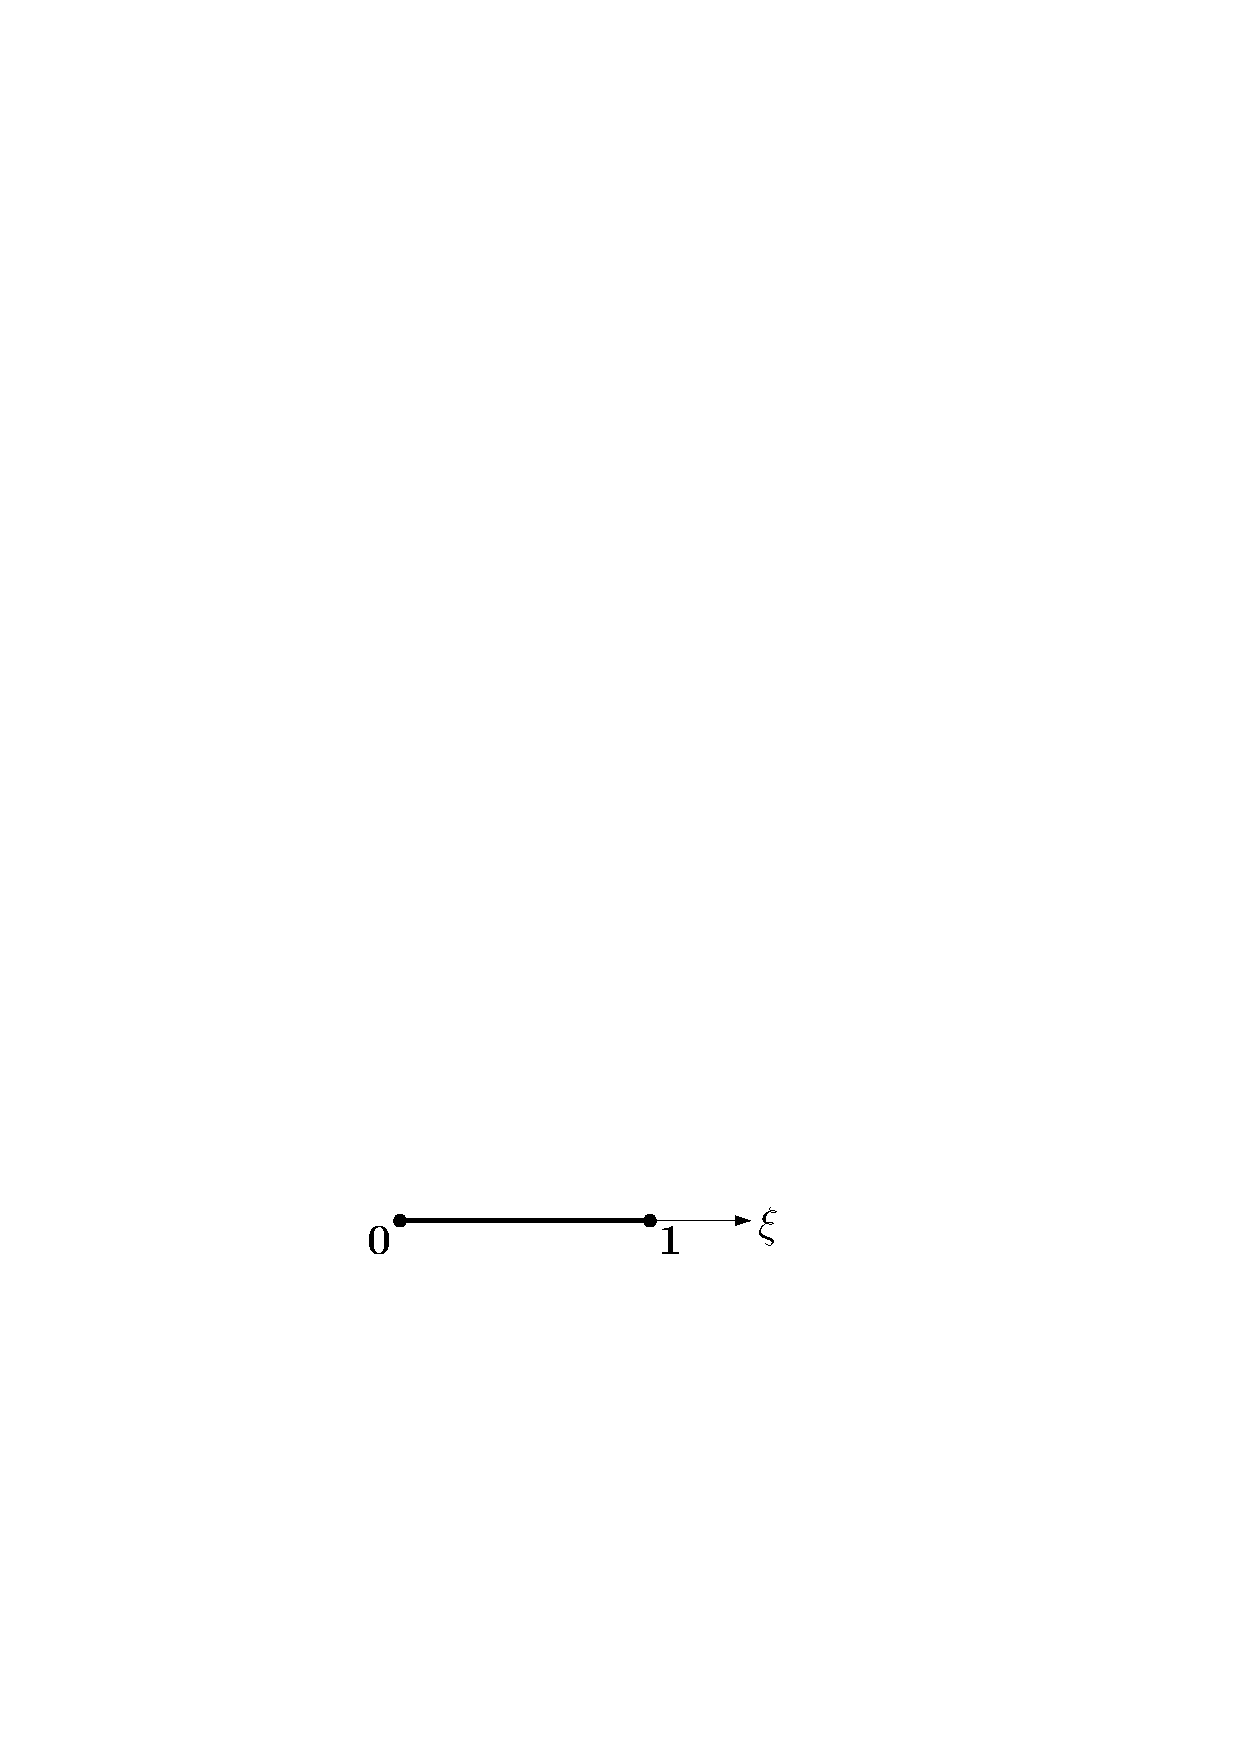
\includegraphics[scale=0.5]{./figures/MasterSegment.pdf}
	\end{center}
\end{minipage}} &\\
\multicolumn{3}{|c|}{Affine Coordinates} &\\
\multicolumn{3}{|c|}{
$	\begin{alignedat}{4}
		\mu_0&=1-\xi\,\qquad\qquad &&\phantom{\nabla}\mu_1&&=\xi\\
		\nabla\mu_0&=-1\,\qquad\qquad &&\nabla\mu_1&&=1
	\end{alignedat}$} &\\
\multicolumn{3}{|c|}{\small\fbox{The order in the pair $\vec{\mu}_{01}=(\mu_0,\mu_1)$ is $p$.}} &\\
\multicolumn{3}{|c|}{} &\\[-17pt]
\hline
\multicolumn{3}{|c|}{$H^1$} &\\
\hline
{}& {} &{} &\\[-23pt]%To keep total width fixed
\multicolumn{2}{|c|}{Shape Functions}& Indices &\\ 
\hline
\multicolumn{2}{|l|}{Vertices} &
\multirow{2}{*}[-12pt]{\small$\begin{gathered}
	a\!=\!0,1
\end{gathered}$} &\\
\multicolumn{2}{|l|}{
$	\begin{aligned}
		\phi^\mathrm{v}&=\mu_a\\
		\nabla\phi^\mathrm{v}&=\nabla\mu_a
	\end{aligned}$} &{}&\\
\multicolumn{2}{|l|}{Edges} &
\multirow{2}{*}[-12pt]{\small$\begin{gathered}
	i\!=\!2,\ldots,p
\end{gathered}$} &\\
\multicolumn{2}{|l|}{
$	\begin{aligned}
		\phi_i^\mathrm{e}&=\phi_i^\E(\vec{\mu}_{01})\,\\
		\nabla\phi_i^\mathrm{e}&=\nabla\phi_i^\E(\vec{\mu}_{01})
	\end{aligned}$} &{}&\\[-17pt]
{}& {} &{} &\\
\hline
\multicolumn{3}{|c|}{$L^2$} &\\
\hline
{}& {} &{} &\\[-23pt]%To keep total width fixed
\multicolumn{2}{|c|}{Shape Functions}& Indices &\\ 
\hline
\multicolumn{2}{|l|}{Edges} &
\multirow{2}{*}[-12pt]{\small$\begin{gathered}
	i\!=\!0,\ldots,p\!-\!1
\end{gathered}$} &\\
\multicolumn{2}{|l|}{
$	\begin{aligned}
		\psi^\mathrm{e}_i=[P_i](\vec{\mu}_{01})\nabla\mu_1
	\end{aligned}$} &{}&\\[-17pt]
{}& {} &{} &\\
\hline
\end{tabular}
\end{center}
\renewcommand{\arraystretch}{1}%Back to normal spacing

\newpage
\subsection{Quadrilateral}

%%%%%%%%%%%%%%%%%%%%%Quadrilateral 1: Geometry,H1%%%%%%%%%%%%%%%%%%%%%
\renewcommand{\arraystretch}{1.35}%Better row spacing
\begin{center}
\begin{tabular}
{|C{0.35cm} L{11.9cm}|C{2.9cm}|N}%See main file for this custom columns - they keep a fixed width while maintaining aligment
\hline
\multicolumn{3}{|c|}{\large \textbf{Quadrilateral}} &\\
\hline
\multicolumn{3}{|c|}{Geometry} &\\
\hline
\multicolumn{3}{|c|}{} &\\[-17pt]
\multicolumn{3}{|c|}{\begin{minipage}{0.9\textwidth}
	\begin{center}
		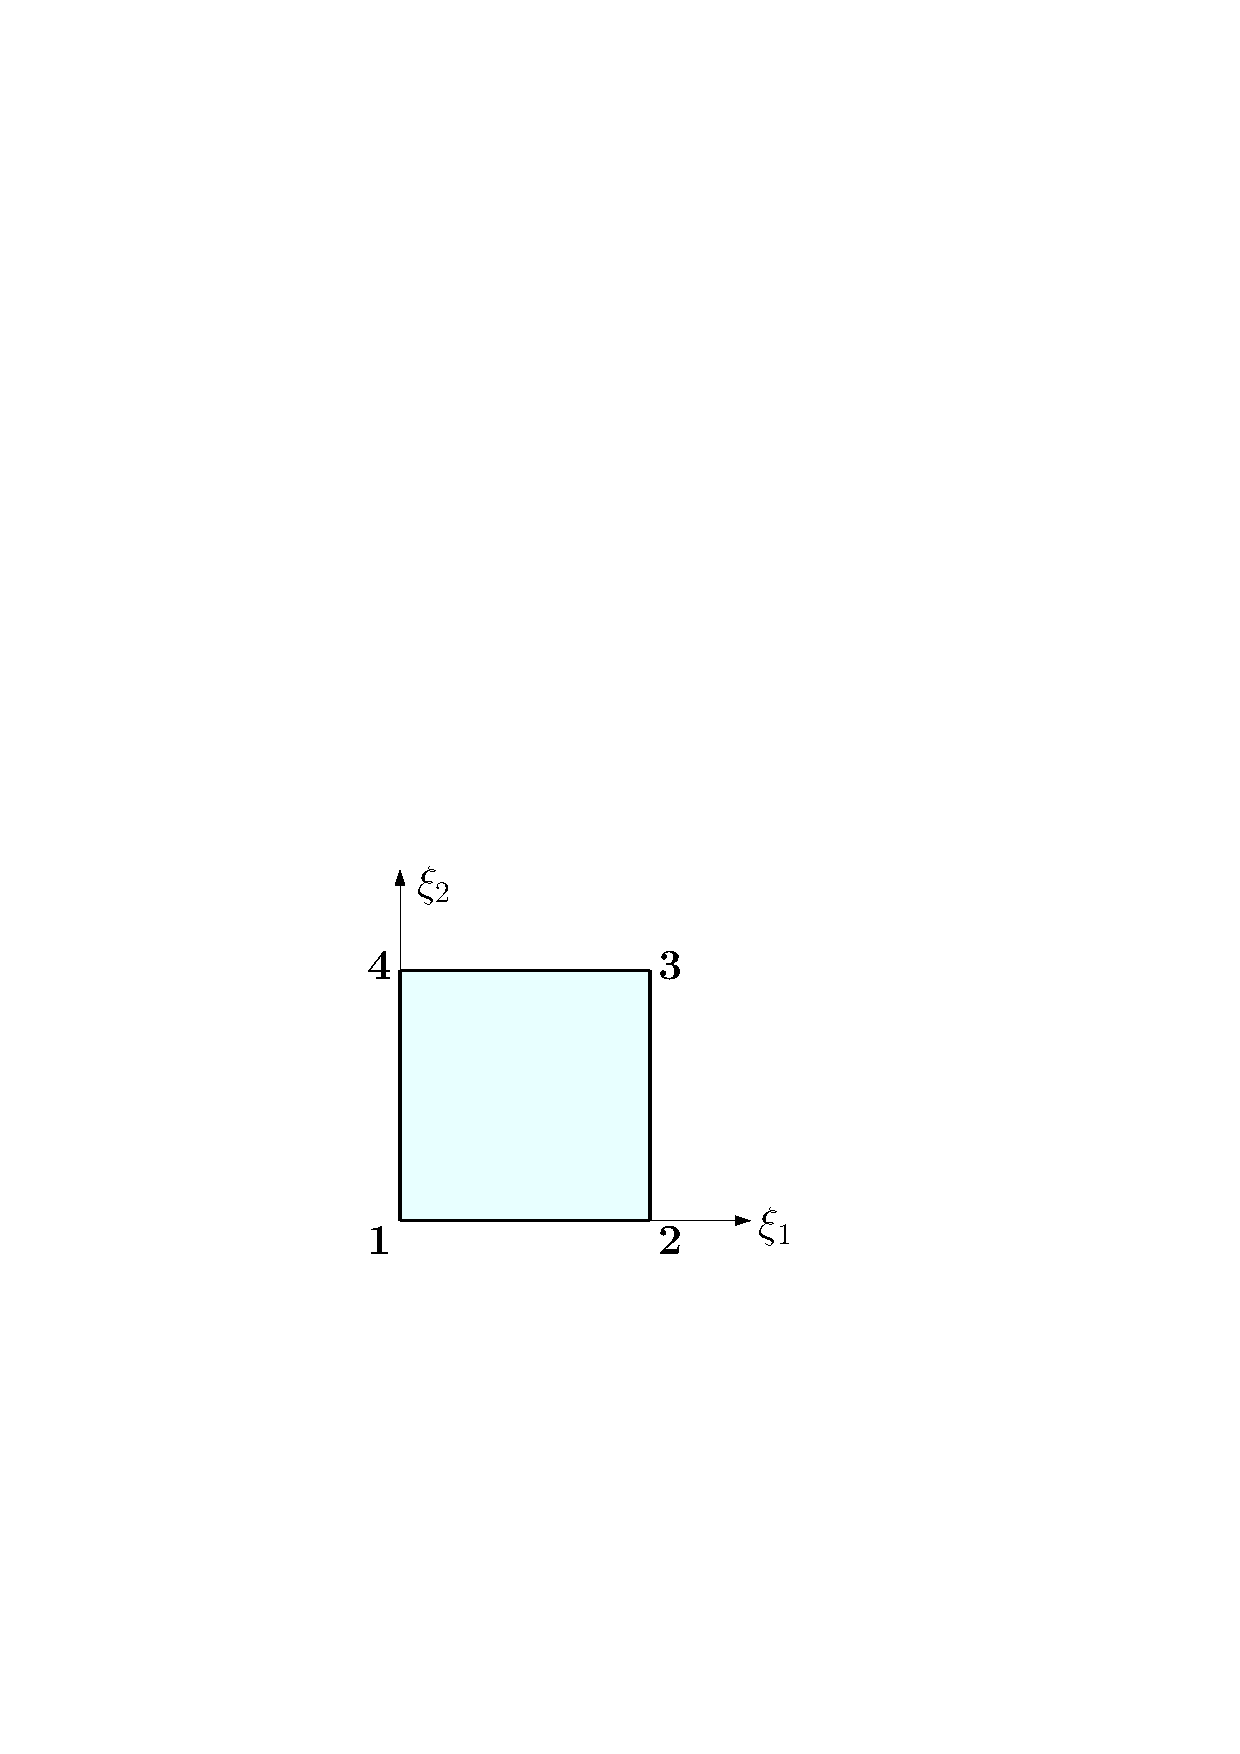
\includegraphics[scale=0.5]{./figures/MasterQuad.pdf}
	\end{center}
\end{minipage}} &\\
\multicolumn{3}{|c|}{Affine Coordinates} &\\
\multicolumn{3}{|c|}{
$	\begin{alignedat}{4}
		\mu_0^{\,\xi_1}&=1-\xi_1\,\qquad\qquad &&\phantom{\nabla}\mu_1^{\,\xi_1}&&=\xi_1\\
		\nabla\mu_0^{\,\xi_1}&=\Big(\begin{smallmatrix}-1\\[2pt]0\end{smallmatrix}\Big)\qquad\qquad 
			&&\nabla\mu_1^{\,\xi_1}&&=\Big(\begin{smallmatrix}1\\[2pt]0\end{smallmatrix}\Big)\\
		\mu_0^{\,\xi_2}&=1-\xi_2\,\qquad\qquad &&\phantom{\nabla}\mu_1^{\,\xi_2}&&=\xi_2\\
		\nabla\mu_0^{\,\xi_2}&=\Big(\begin{smallmatrix}0\\[2pt]-1\end{smallmatrix}\Big)\qquad\qquad 
			&&\nabla\mu_1^{\,\xi_2}&&=\Big(\begin{smallmatrix}0\\[2pt]1\end{smallmatrix}\Big)
	\end{alignedat}$} &\\
\multicolumn{3}{|c|}{} &\\[-17pt]
\multicolumn{3}{|c|}{\small\fbox{\parbox[c][25pt][c]{0.4\textwidth}{The order in the pair $\vec{\mu}_{01}^{\,\xi_1}=(\mu_0^{\,\xi_1},\mu_1^{\,\xi_1})$ is $p_1$.\\The order in the pair $\vec{\mu}_{01}^{\,\xi_2}=(\mu_0^{\,\xi_2},\mu_1^{\,\xi_2})$ is $p_2$.}}} &\\
\multicolumn{3}{|c|}{} &\\[-17pt]
\hline
\multicolumn{3}{|c|}{$H^1$} &\\
\hline
{}& {} &{} &\\[-23pt]%To keep total width fixed
\multicolumn{2}{|c|}{Shape Functions}& Indices &\\ 
\hline
\multicolumn{2}{|l|}{Vertices} &
\multirow{2}{*}[-12pt]{\small$\begin{gathered}
	a\!=\!0,1,\,b\!=\!0,1
\end{gathered}$} &\\
\multicolumn{2}{|l|}{
$	\begin{aligned}
		\phi^\mathrm{v}&=\mu_a^{\,\xi_1}\mu_b^{\,\xi_2}\\
		\nabla\phi^\mathrm{v}&=\mu_a^{\,\xi_1}\nabla\mu_b^{\,\xi_2}+\mu_b^{\,\xi_2}\nabla\mu_a^{\,\xi_1}
	\end{aligned}$} &{}&\\
\multicolumn{2}{|l|}{Edges} &
\multirow{2}{*}[-12pt]{\small$\begin{gathered}
	i\!=\!2,\ldots,p_a\\
	(a,b)\!=\!(1,2),(2,1)\\
	c\!=\!0,1
\end{gathered}$} &\\
\multicolumn{2}{|l|}{
$	\begin{aligned}
		\phi_i^\mathrm{e}&=\mu_c^{\,\xi_b}\phi_i^\E(\vec{\mu}_{01}^{\,\xi_a})\\
		\nabla\phi_i^\mathrm{e}&=\mu_c^{\,\xi_b}\nabla\phi_i^\E(\vec{\mu}_{01}^{\,\xi_a})
        +\phi_i^\E(\vec{\mu}_{01}^{\,\xi_a})\nabla\mu_c^{\,\xi_b}
	\end{aligned}$} &{}&\\
\multicolumn{2}{|l|}{Face} &
\multirow{2}{*}[-12pt]{\small$\begin{gathered}
	i\!=\!2,\ldots,p_1\\
	j\!=\!2,\ldots,p_2
\end{gathered}$} &\\
\multicolumn{2}{|l|}{
$	\begin{aligned}
		\phi_{ij}^\mathrm{f}&=\phi_{ij}^\square(\vec{\mu}_{01}^{\,\xi_1},\vec{\mu}_{01}^{\,\xi_2})\\
		\nabla\phi_{ij}^\mathrm{f}&=\nabla\phi_{ij}^\square(\vec{\mu}_{01}^{\,\xi_1},\vec{\mu}_{01}^{\,\xi_2})
	\end{aligned}$} &{}&\\[-17pt]
{}& {} &{} &\\[-5pt]
\multicolumn{3}{r}{\footnotesize\textit{continued on next page}} &\\[-18.5pt]
\hline
\end{tabular}
\end{center}
\renewcommand{\arraystretch}{1}%Back to normal spacing

\newpage

%%%%%%%%%%%%%%%%%%%%%Quadrilateral 2: Hcurl,Hdiv%%%%%%%%%%%%%%%%%%%%%
\renewcommand{\arraystretch}{1.35}%Better row spacing
\begin{center}
\begin{tabular}
{|C{0.35cm} L{11.9cm}|C{2.9cm}|N}%See main file for this custom columns - they keep a fixed width while maintaining aligment
\multicolumn{3}{l}{\footnotesize\textit{continued from previous page}} &\\[-2pt]
\hline
\multicolumn{3}{|c|}{\large \textbf{Quadrilateral}} &\\
\hline
\multicolumn{3}{|c|}{$H(\mathrm{curl})^\star$} &\\
\hline
{}& {} &{} &\\[-23pt]%To keep total width fixed
\multicolumn{2}{|c|}{Shape Functions}& Indices &\\ 
\hline
\multicolumn{2}{|l|}{Edges} &
\multirow{2}{*}[-12pt]{\small$\begin{gathered}
	i\!=\!0,\ldots,p_a\!-\!1\\
	(a,b)\!=\!(1,2),(2,1)\\
	c\!=\!0,1
\end{gathered}$} &\\
\multicolumn{2}{|l|}{
$	\begin{aligned}
		E_i^\mathrm{e}&=\mu_c^{\,\xi_b}E_i^\E(\vec{\mu}_{01}^{\,\xi_a})\\
		\nabla\!\times\! E_i^\mathrm{e}&=\nabla\mu_c^{\,\xi_b}\!\times\! E_i^\E(\vec{\mu}_{01}^{\,\xi_a})
	\end{aligned}$} &{}&\\
\multicolumn{2}{|l|}{Face} & {}&\\
\multicolumn{2}{|l|}{\small $\,$Family I} &
\multirow{2}{*}[-12pt]{\small$\begin{gathered}
	i\!=\!0,\ldots,p_1\!-\!1\\
	j\!=\!2,\ldots,p_2
\end{gathered}$} &\\
\multicolumn{2}{|l|}{
$	\begin{aligned}
		E_{ij}^{\mathrm{f}}&=E_{ij}^{\square}(\vec{\mu}_{01}^{\,\xi_1},\vec{\mu}_{01}^{\,\xi_2})\\
		\nabla\!\times\! E_{ij}^{\mathrm{f}}&=\nabla\!\times\! E_{ij}^{\square}(\vec{\mu}_{01}^{\,\xi_1},\vec{\mu}_{01}^{\,\xi_2})
	\end{aligned}$} &{}&\\
\multicolumn{2}{|l|}{\small $\,$Family II} &
\multirow{2}{*}[-12pt]{\small$\begin{gathered}
	i\!=\!0,\ldots,p_2\!-\!1\\
	j\!=\!2,\ldots,p_1
\end{gathered}$} &\\
\multicolumn{2}{|l|}{
$	\begin{aligned}
		E_{ij}^{\mathrm{f}}&=E_{ij}^{\square}(\vec{\mu}_{01}^{\,\xi_2},\vec{\mu}_{01}^{\,\xi_1})\\
		\nabla\!\times\! E_{ij}^{\mathrm{f}}&=\nabla\!\times\! E_{ij}^{\square}(\vec{\mu}_{01}^{\,\xi_2},\vec{\mu}_{01}^{\,\xi_1})
	\end{aligned}$} &{}&\\[-17pt]
{}& {} &{} &\\
\hline
\multicolumn{3}{|c|}{$H(\mathrm{div})$} &\\
\hline
{}& {} &{} &\\[-23pt]%To keep total width fixed
\multicolumn{2}{|c|}{Shape Functions}& Indices &\\ 
\hline
\multicolumn{2}{|l|}{\parbox[c][35pt][l]{0.75\textwidth}{For any given topological entity, the $H(\mathrm{div})$ shape functions are the rotation of the corresponding $H(\mathrm{curl})$ shape functions:}}& {} &\\[30pt]
\multicolumn{2}{|l|}{
$	\begin{aligned}
		V&=\Big(\begin{smallmatrix}0&1\\[2pt]-1&0\end{smallmatrix}\Big)E\\
		\nabla\!\cdot\! V&=\nabla\!\times\! E
	\end{aligned}$} &{}&\\[-17pt]
{}& {} &{} &\\
\hline
\multicolumn{3}{|c|}{$L^2$} &\\
\hline
{}& {} &{} &\\[-23pt]%To keep total width fixed
\multicolumn{2}{|c|}{Shape Functions}& Indices &\\ 
\hline
\multicolumn{2}{|l|}{Face} &
\multirow{2}{*}[-5pt]{\small$\begin{gathered}
	i\!=\!0,\ldots,p_1\!-\!1\\
	j\!=\!0,\ldots,p_2\!-\!1
\end{gathered}$} &\\
\multicolumn{2}{|l|}{
$	\begin{aligned}
		\psi_{ij}^\mathrm{f}=[P_i](\vec{\mu}_{01}^{\,\xi_1})[P_j](\vec{\mu}_{01}^{\,\xi_2})
			(\nabla\mu_1^{\,\xi_1}\!\times\!\nabla\mu_1^{\,\xi_2})
	\end{aligned}$} &{}&\\[-4pt]
\multicolumn{3}{|c|}{} &\\[-11.25pt]
\multicolumn{3}{|c|}{} &\\[-47.75pt]
{}& {} &{} &\\
\hline
\multicolumn{3}{r}{} &\\[-18.5pt]
\multicolumn{3}{l}{\multirow{1}{*}[4pt]{\footnotesize $\star$ In 2D the curl and cross product are $\nabla\!\times\!\Big(\begin{smallmatrix}E_1\\[2pt]E_2\end{smallmatrix}\Big)
        =\frac{\partial E_2}{\partial \xi_1}-\frac{\partial E_1}{\partial \xi_2}$ and $\Big(\begin{smallmatrix}E_1\\[2pt]E_2\end{smallmatrix}\Big)\!\times\!\Big(\begin{smallmatrix}F_1\\[2pt]F_2\end{smallmatrix}\Big)=E_1F_2-E_2F_1$ respectively.}} &\\[-8.5pt]
\multicolumn{3}{r}{} &\\[-18.5pt]
\hline
\end{tabular}
\end{center}
\renewcommand{\arraystretch}{1}%Back to normal spacing

\newpage
\subsection{Triangle}

%%%%%%%%%%%%%%%%%%%%%Triangle 1: Geometry,H1%%%%%%%%%%%%%%%%%%%%%
\renewcommand{\arraystretch}{1.35}%Better row spacing
\begin{center}
\begin{tabular}
{|C{0.35cm} L{11.9cm}|C{2.9cm}|N}%See main file for this custom columns - they keep a fixed width while maintaining aligment
\hline
\multicolumn{3}{|c|}{\large \textbf{Triangle}} &\\
\hline
\multicolumn{3}{|c|}{Geometry} &\\
\hline
\multicolumn{3}{|c|}{} &\\[-17pt]
\multicolumn{3}{|c|}{\begin{minipage}{0.9\textwidth}
	\begin{center}
		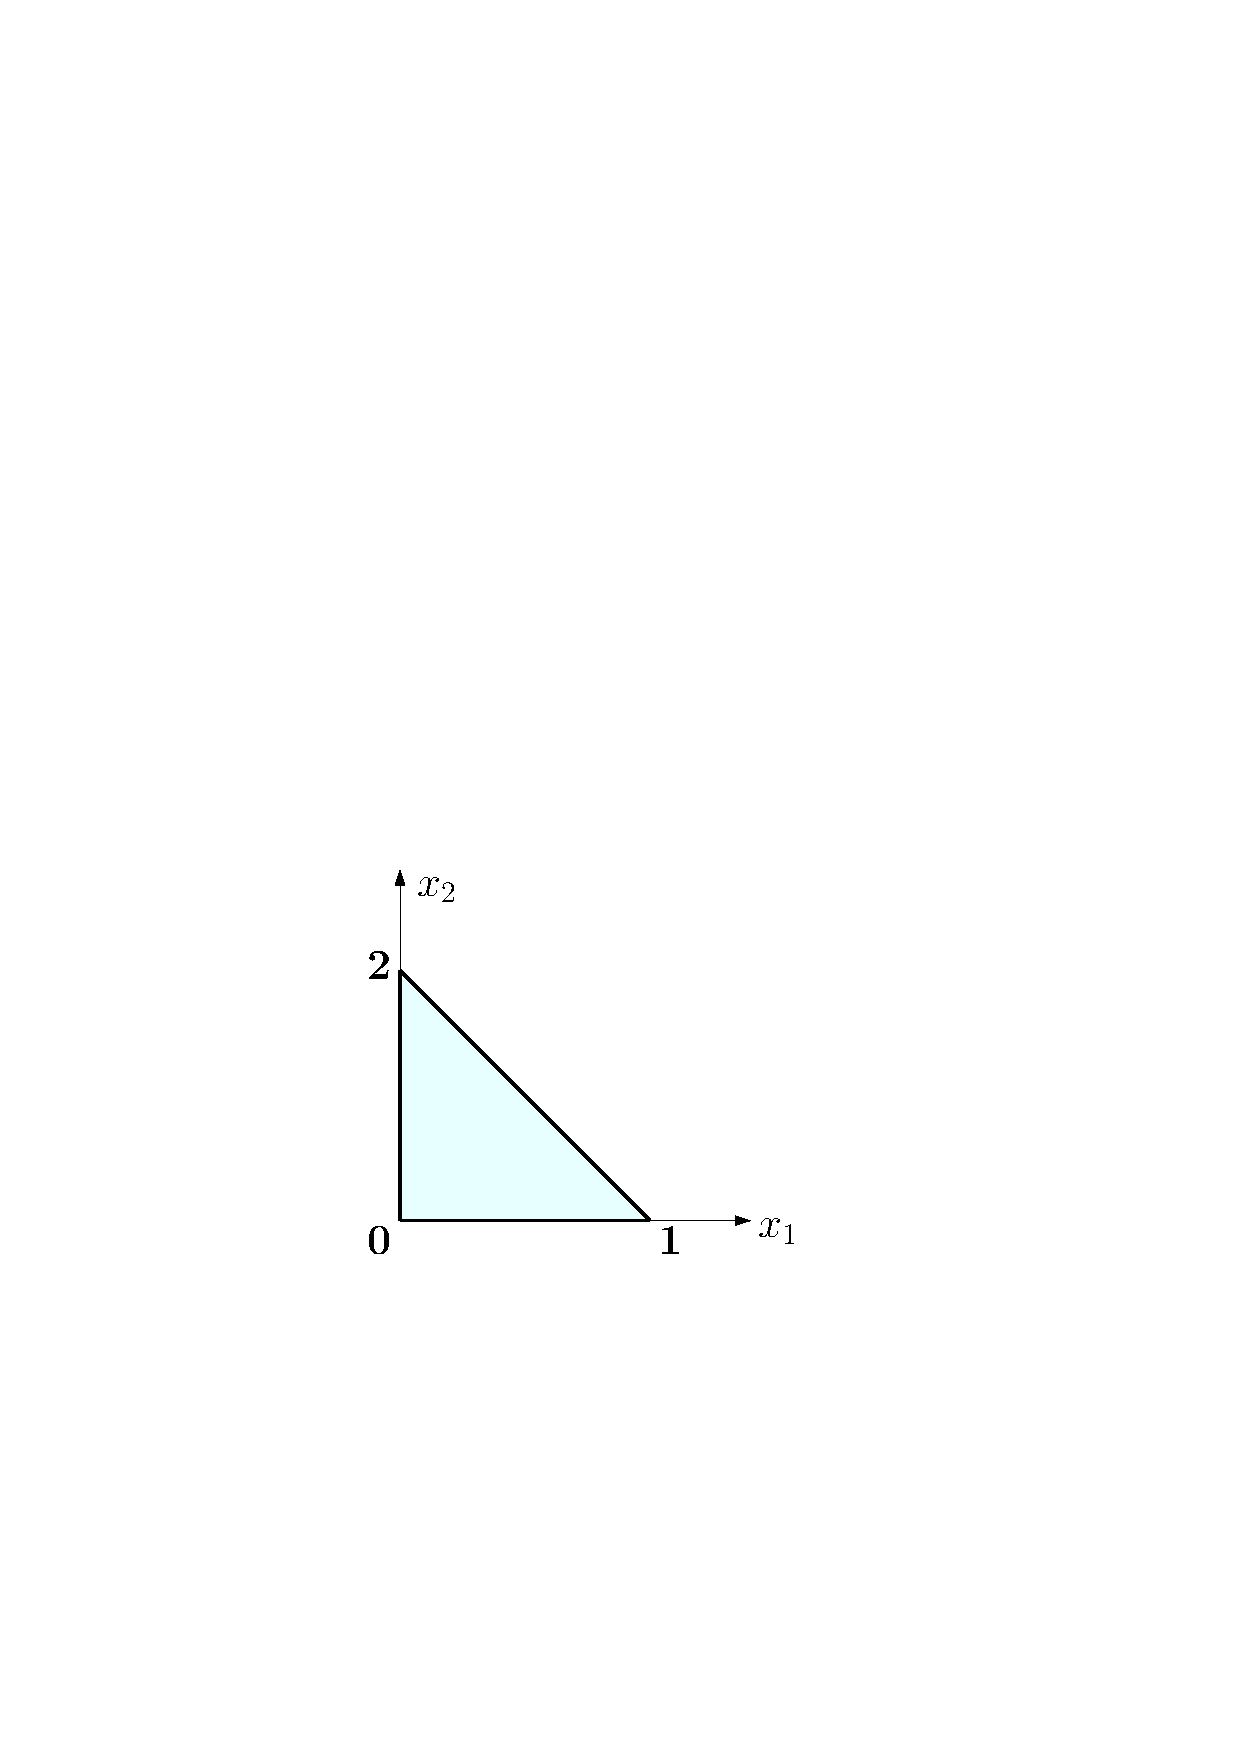
\includegraphics[scale=0.5]{./figures/MasterTri.pdf}
	\end{center}
\end{minipage}} &\\
\multicolumn{3}{|c|}{Affine Coordinates} &\\
\multicolumn{3}{|c|}{
$	\begin{alignedat}{6}
		\nu_0&=1-x_1-x_2\,\qquad\qquad &&\phantom{\nabla}\nu_1&&=x_1\qquad\qquad &&\phantom{\nabla}\nu_2&&=x_2\\
		\nabla\nu_0&=\Big(\begin{smallmatrix}-1\\[2pt]-1\end{smallmatrix}\Big)\qquad\qquad 
			&&\nabla\nu_1&&=\Big(\begin{smallmatrix}1\\[2pt]0\end{smallmatrix}\Big)\qquad\qquad 
				&&\nabla\nu_2&&=\Big(\begin{smallmatrix}0\\[2pt]1\end{smallmatrix}\Big)
	\end{alignedat}$} &\\
\multicolumn{3}{|c|}{} &\\[-17pt]
\multicolumn{3}{|c|}{\small\fbox{The order in the triplet $\vec{\nu}_{012}=(\nu_0,\nu_1,\nu_2)$ and all its subpairs is $p$.}} &\\
\multicolumn{3}{|c|}{} &\\[-17pt]
\hline
\multicolumn{3}{|c|}{$H^1$} &\\
\hline
{}& {} &{} &\\[-23pt]%To keep total width fixed
\multicolumn{2}{|c|}{Shape Functions}& Indices &\\ 
\hline
\multicolumn{2}{|l|}{Vertices} &
\multirow{2}{*}[-12pt]{\small$\begin{gathered}
	a\!=\!0,1,2
\end{gathered}$} &\\
\multicolumn{2}{|l|}{
$	\begin{aligned}
		\phi^\mathrm{v}&=\nu_a\\
		\nabla\phi^\mathrm{v}&=\nabla\nu_a
	\end{aligned}$} &{}&\\
\multicolumn{2}{|l|}{Edges} &
\multirow{2}{*}[-12pt]{\small$\begin{gathered}
	i\!=\!2,\ldots,p\\
	0\leq a<b\leq2
\end{gathered}$} &\\
\multicolumn{2}{|l|}{
$	\begin{aligned}
		\phi_i^\mathrm{e}&=\phi_i^\E(\vec{\nu}_{ab})\\
		\nabla\phi_i^\mathrm{e}&=\nabla\phi_i^\E(\vec{\nu}_{ab})
	\end{aligned}$} &{}&\\
\multicolumn{2}{|l|}{Face} &
\multirow{2}{*}[-12pt]{\small$\begin{gathered}
	i\geq2,\,j\geq1\\
	i\!+\!j\!=\!3,\ldots,p
\end{gathered}$} &\\
\multicolumn{2}{|l|}{
$	\begin{aligned}
		\phi_{ij}^\mathrm{f}&=\phi_{ij}^\Tri(\vec{\nu}_{012})\\
		\nabla\phi_{ij}^\mathrm{f}&=\nabla\phi_{ij}^\Tri(\vec{\nu}_{012})
	\end{aligned}$} &{}&\\[-17pt]
{}& {} &{} &\\[-5pt]
\multicolumn{3}{r}{\footnotesize\textit{continued on next page}} &\\[-18.5pt]
\hline
\end{tabular}
\end{center}
\renewcommand{\arraystretch}{1}%Back to normal spacing

\newpage

%%%%%%%%%%%%%%%%%%%%%Triangle 2: Hcurl,Hdiv%%%%%%%%%%%%%%%%%%%%%
\renewcommand{\arraystretch}{1.35}%Better row spacing
\begin{center}
\begin{tabular}
{|C{0.35cm} L{11.9cm}|C{2.9cm}|N}%See main file for this custom columns - they keep a fixed width while maintaining aligment
\multicolumn{3}{l}{\footnotesize\textit{continued from previous page}} &\\[-2pt]
\hline
\multicolumn{3}{|c|}{\large \textbf{Triangle}} &\\
\hline
\multicolumn{3}{|c|}{$H(\mathrm{curl})^\star$} &\\
\hline
{}& {} &{} &\\[-23pt]%To keep total width fixed
\multicolumn{2}{|c|}{Shape Functions}& Indices &\\ 
\hline
\multicolumn{2}{|l|}{Edges} &
\multirow{2}{*}[-12pt]{\small$\begin{gathered}
	i\!=\!0,\ldots,p\!-\!1\\
	0\leq a<b\leq2
\end{gathered}$} &\\
\multicolumn{2}{|l|}{
$	\begin{aligned}
		E_i^\mathrm{e}&=E_i^\E(\vec{\nu}_{ab})\\
		\nabla\!\times\! E_i^\mathrm{e}&=\nabla\!\times\! E_i^\E(\vec{\nu}_{ab})
	\end{aligned}$} &{}&\\
\multicolumn{2}{|l|}{Face} & {}&\\
\multicolumn{2}{|l|}{\small $\,$Family I} &
\multirow{2}{*}[-12pt]{\small$\begin{gathered}
	i\geq0,\,j\geq1\\
	i\!+\!j\!=\!1,\ldots,p\!-\!1
\end{gathered}$} &\\
\multicolumn{2}{|l|}{
$	\begin{aligned}
		E_{ij}^{\mathrm{f}}&=E_{ij}^\Tri(\vec{\nu}_{012})\\
		\nabla\!\times\! E_{ij}^{\mathrm{f}}&=\nabla\!\times\! E_{ij}^\Tri(\vec{\nu}_{012})
	\end{aligned}$} &{}&\\
\multicolumn{2}{|l|}{\small $\,$Family II} &
\multirow{2}{*}[-12pt]{\small$\begin{gathered}
	i\geq0,\,j\geq1\\
	i\!+\!j\!=\!1,\ldots,p\!-\!1
\end{gathered}$} &\\
\multicolumn{2}{|l|}{
$	\begin{aligned}
		E_{ij}^{\mathrm{f}}&=E_{ij}^\Tri(\vec{\nu}_{120})\\
		\nabla\!\times\! E_{ij}^{\mathrm{f}}&=\nabla\!\times\! E_{ij}^\Tri(\vec{\nu}_{120})
	\end{aligned}$} &{}&\\[-17pt]
{}& {} &{} &\\
\hline
\multicolumn{3}{|c|}{$H(\mathrm{div})$} &\\
\hline
{}& {} &{} &\\[-23pt]%To keep total width fixed
\multicolumn{2}{|c|}{Shape Functions}& Indices &\\ 
\hline
\multicolumn{2}{|l|}{\parbox[c][35pt][l]{0.75\textwidth}{For any given topological entity, the $H(\mathrm{div})$ shape functions are the rotation of the corresponding $H(\mathrm{curl})$ shape functions:}}& {} &\\[30pt]
\multicolumn{2}{|l|}{
$	\begin{aligned}
		V&=\Big(\begin{smallmatrix}0&1\\[2pt]-1&0\end{smallmatrix}\Big)E\\
		\nabla\!\cdot\! V&=\nabla\!\times\! E
	\end{aligned}$} &{}&\\[-17pt]
{}& {} &{} &\\
\hline
\multicolumn{3}{|c|}{$L^2$} &\\
\hline
{}& {} &{} &\\[-23pt]%To keep total width fixed
\multicolumn{2}{|c|}{Shape Functions}& Indices &\\ 
\hline
\multicolumn{2}{|l|}{Face} &
\multirow{2}{*}[-5pt]{\small$\begin{gathered}
	i\geq0,\,j\geq0\\
	i\!+\!j\!=\!0,\ldots,p\!-\!1
\end{gathered}$} &\\
\multicolumn{2}{|l|}{
$	\begin{aligned}
		\psi_{ij}^\mathrm{f}=[P_i](\vec{\nu}_{01})[P_j^{2i+1}](\nu_0+\nu_1,\nu_2)
			(\nabla\nu_1\!\times\!\nabla\nu_2)
	\end{aligned}$} &{}&\\[-4pt]
\multicolumn{3}{|c|}{} &\\[-11.25pt]
\multicolumn{3}{|c|}{} &\\[-47.75pt]
{}& {} &{} &\\
\hline
\multicolumn{3}{r}{} &\\[-18.5pt]
\multicolumn{3}{l}{\multirow{1}{*}[4pt]{\footnotesize $\star$ In 2D the curl and cross product are $\nabla\!\times\!\Big(\begin{smallmatrix}E_1\\[2pt]E_2\end{smallmatrix}\Big)
        =\frac{\partial E_2}{\partial x_1}-\frac{\partial E_1}{\partial x_2}$ and $\Big(\begin{smallmatrix}E_1\\[2pt]E_2\end{smallmatrix}\Big)\!\times\!\Big(\begin{smallmatrix}F_1\\[2pt]F_2\end{smallmatrix}\Big)=E_1F_2-E_2F_1$ respectively.}} &\\[-8.5pt]
\multicolumn{3}{r}{} &\\[-18.5pt]
\hline
\end{tabular}
\end{center}
\renewcommand{\arraystretch}{1}%Back to normal spacing

\newpage
\subsection{Hexahedron}

%%%%%%%%%%%%%%%%%%%%%Hexahedron 1: Geometry%%%%%%%%%%%%%%%%%%%%%
\renewcommand{\arraystretch}{1.35}%Better row spacing
\begin{center}
\begin{tabular}
{|C{0.35cm} L{11.9cm} C{2.9cm}|N}%See main file for this custom columns - they keep a fixed width while maintaining aligment
\hline
\multicolumn{3}{|c|}{\large \textbf{Hexahedron}} &\\
\hline
\multicolumn{3}{|c|}{Geometry} &\\
\hline
\multicolumn{3}{|c|}{} &\\[-10pt]
\multicolumn{3}{|c|}{\begin{minipage}{0.9\textwidth}
	\begin{center}
		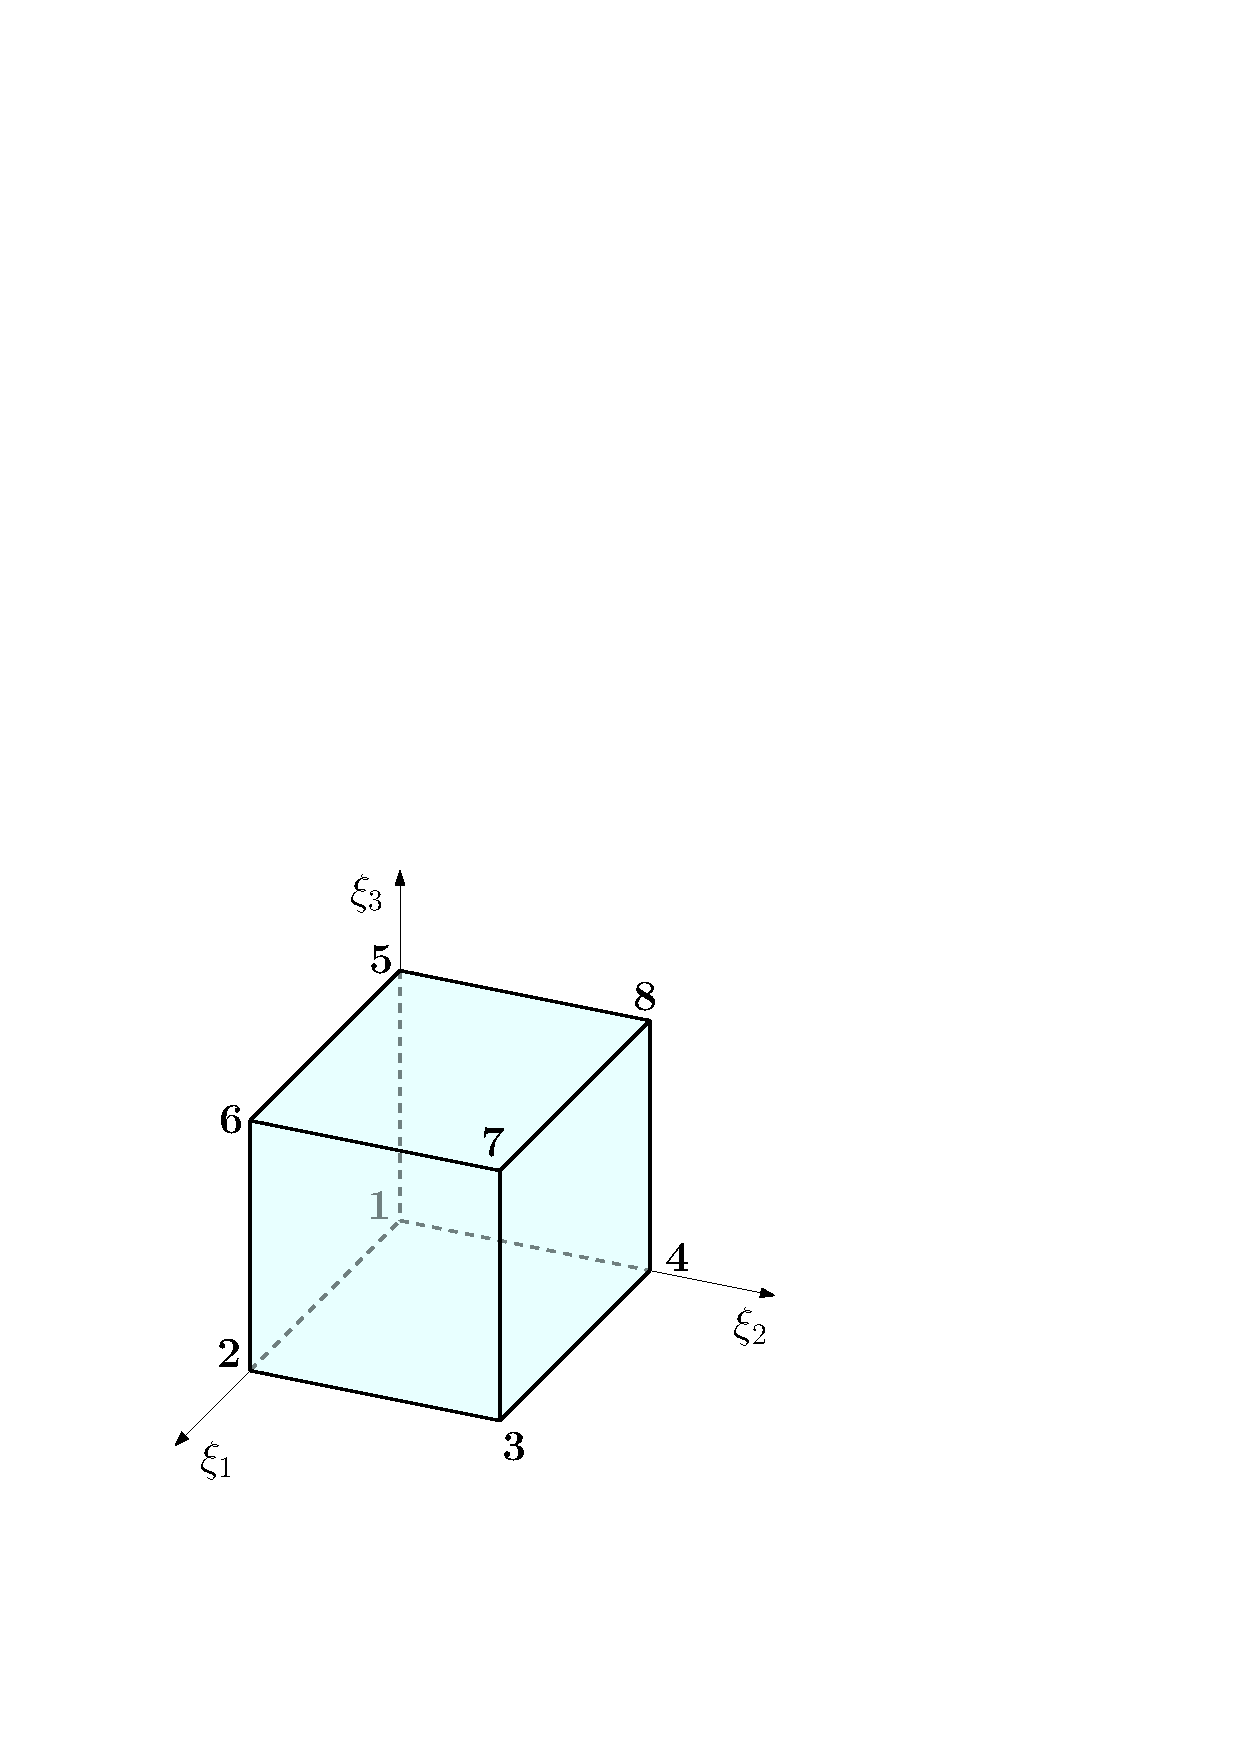
\includegraphics[scale=0.5]{./figures/MasterHexa.pdf}
	\end{center}
\end{minipage}} &\\
\multicolumn{3}{|c|}{Affine Coordinates} &\\
\multicolumn{3}{|c|}{
$	\begin{alignedat}{4}
		\mu_0^{\,\xi_1}&=1-\xi_1\,\qquad\qquad &&\phantom{\nabla}\mu_1^{\,\xi_1}&&=\xi_1\\
		\nabla\mu_0^{\,\xi_1}&=\bigg(\begin{smallmatrix}-1\\[2pt]0\\[2pt]0\end{smallmatrix}\bigg)\qquad\qquad 
			&&\nabla\mu_1^{\,\xi_1}&&=\bigg(\begin{smallmatrix}1\\[2pt]0\\[2pt]0\end{smallmatrix}\bigg)\\
		\mu_0^{\,\xi_2}&=1-\xi_2\,\qquad\qquad &&\phantom{\nabla}\mu_1^{\,\xi_2}&&=\xi_2\\
		\nabla\mu_0^{\,\xi_2}&=\bigg(\begin{smallmatrix}0\\[2pt]-1\\[2pt]0\end{smallmatrix}\bigg)\qquad\qquad 
			&&\nabla\mu_1^{\,\xi_2}&&=\bigg(\begin{smallmatrix}0\\[2pt]1\\[2pt]0\end{smallmatrix}\bigg)\\
		\mu_0^{\,\xi_3}&=1-\xi_3\,\qquad\qquad &&\phantom{\nabla}\mu_1^{\,\xi_3}&&=\xi_3\\
		\nabla\mu_0^{\,\xi_3}&=\bigg(\begin{smallmatrix}0\\[2pt]0\\[2pt]-1\end{smallmatrix}\bigg)\qquad\qquad 
			&&\nabla\mu_1^{\,\xi_3}&&=\bigg(\begin{smallmatrix}0\\[2pt]0\\[2pt]1\end{smallmatrix}\bigg)
	\end{alignedat}$} &\\
\multicolumn{3}{|c|}{} &\\[-7pt]
\multicolumn{3}{|c|}{\small\fbox{\parbox[c][40pt][c]{0.4\textwidth}{The order in the pair $\vec{\mu}_{01}^{\,\xi_1}=(\mu_0^{\,\xi_1},\mu_1^{\,\xi_1})$ is $p_1$.\\The order in the pair $\vec{\mu}_{01}^{\,\xi_2}=(\mu_0^{\,\xi_2},\mu_1^{\,\xi_2})$ is $p_2$.\\The order in the pair $\vec{\mu}_{01}^{\,\xi_3}=(\mu_0^{\,\xi_3},\mu_1^{\,\xi_3})$ is $p_3$.}}} &\\
\multicolumn{3}{|c|}{} &\\[-17pt]
{}& {} &{} &\\[-5pt]
\multicolumn{3}{r}{\footnotesize\textit{continued on next page}} &\\[-18.5pt]
\hline
\end{tabular}
\end{center}
\renewcommand{\arraystretch}{1}%Back to normal spacing

\newpage

%%%%%%%%%%%%%%%%%%%%%Hexahedron 2: H1%%%%%%%%%%%%%%%%%%%%%
\renewcommand{\arraystretch}{1.35}%Better row spacing
\begin{center}
\begin{tabular}
{|C{0.35cm} L{11.9cm}|C{2.9cm}|N}%See main file for this custom columns - they keep a fixed width while maintaining aligment
\multicolumn{3}{l}{\footnotesize\textit{continued from previous page}} &\\[-2pt]
\hline
\multicolumn{3}{|c|}{\large \textbf{Hexahedron}} &\\
\hline
\multicolumn{3}{|c|}{$H^1$} &\\
\hline
{}& {} &{} &\\[-23pt]%To keep total width fixed
\multicolumn{2}{|c|}{Shape Functions}& Indices &\\ 
\hline
\multicolumn{2}{|l|}{Vertices} &
\multirow{2}{*}[-12pt]{\small$\begin{gathered}
	a\!=\!0,1,\,b\!=\!0,1\\
	c\!=\!0,1
\end{gathered}$} &\\
\multicolumn{2}{|l|}{
$	\begin{aligned}
		\phi^\mathrm{v}&=\mu_a^{\,\xi_1}\mu_b^{\,\xi_2}\mu_c^{\,\xi_3}\\
		\nabla\phi^\mathrm{v}&=\mu_a^{\,\xi_1}\mu_b^{\,\xi_2}\nabla\mu_c^{\,\xi_3}+\mu_c^{\,\xi_3}\mu_a^{\,\xi_1}\nabla\mu_b^{\,\xi_2}
			+\mu_b^{\,\xi_2}\mu_c^{\,\xi_3}\nabla\mu_a^{\,\xi_1}
	\end{aligned}$} &{}&\\
\multicolumn{2}{|l|}{Edges} &
\multirow{2}{*}[-12pt]{\small$\begin{gathered}
	i\!=\!2,\ldots,p_a\\[-2pt]
	(a,b,c)\!=\!(1,2,3),\\[-2pt]
	(2,3,1),(3,1,2)\\[-2pt]
	d\!=\!0,1,\,e\!=\!0,1,
\end{gathered}$} &\\
\multicolumn{2}{|l|}{
$	\begin{aligned}
		\phi_i^\mathrm{e}&=\mu_e^{\,\xi_c}\mu_d^{\,\xi_b}\phi_i^\E(\vec{\mu}_{01}^{\,\xi_a})\\
		\nabla\phi_i^\mathrm{e}&=\mu_e^{\,\xi_c}\mu_d^{\,\xi_b}\nabla\phi_i^\E(\vec{\mu}_{01}^{\,\xi_a})
			+\phi_i^\E(\vec{\mu}_{01}^{\,\xi_a})\Big(\mu_e^{\,\xi_c}\nabla\mu_d^{\,\xi_b}+\mu_d^{\,\xi_b}\nabla\mu_e^{\,\xi_c}\Big)
	\end{aligned}$} &{}&\\[30pt]
\multicolumn{2}{|l|}{Faces} &
\multirow{2}{*}[-9pt]{\small$\begin{gathered}
	i\!=\!2,\ldots,p_a\\[-2pt]
	j\!=\!2,\ldots,p_b\\[-2pt]
	(a,b,c)\!=\!(1,2,3),\\[-2pt]
	(2,3,1),(3,1,2)\\[-2pt]
	d\!=\!0,1
\end{gathered}$} &\\
\multicolumn{2}{|l|}{
$	\begin{aligned}
		\phi_{ij}^\mathrm{f}&=\mu_d^{\,\xi_c}\phi_{ij}^\square(\vec{\mu}_{01}^{\,\xi_a},\vec{\mu}_{01}^{\,\xi_b})\\
		\nabla\phi_{ij}^\mathrm{f}&=\mu_d^{\,\xi_c}\nabla\phi_{ij}^\square(\vec{\mu}_{01}^{\,\xi_a},\vec{\mu}_{01}^{\,\xi_b})
			+\phi_{ij}^\square(\vec{\mu}_{01}^{\,\xi_a},\vec{\mu}_{01}^{\,\xi_b})\nabla\mu_d^{\,\xi_c}
	\end{aligned}$} &{}&\\[35pt]
\multicolumn{2}{|l|}{Interior} &
\multirow{2}{*}[-12pt]{\small$\begin{gathered}
	i\!=\!2,\ldots,p_1\\[-2pt]
	j\!=\!2,\ldots,p_2\\[-2pt]
	k\!=\!2,\ldots,p_3
\end{gathered}$} &\\
\multicolumn{2}{|l|}{
$	\begin{aligned}
		\phi_{ijk}^\mathrm{b}&=\phi_{ij}^\square(\vec{\mu}_{01}^{\,\xi_1},\vec{\mu}_{01}^{\,\xi_2})\phi_k^\E(\vec{\mu}_{01}^{\,\xi_3})\\
		\nabla\phi_{ijk}^\mathrm{b}&=
			\phi_{ij}^\square(\vec{\mu}_{01}^{\,\xi_1},\vec{\mu}_{01}^{\,\xi_2})\nabla\phi_k^\E(\vec{\mu}_{01}^{\,\xi_3})
				+\phi_k^\E(\vec{\mu}_{01}^{\,\xi_3})\nabla\phi_{ij}^\square(\vec{\mu}_{01}^{\,\xi_1},\vec{\mu}_{01}^{\,\xi_2})
	\end{aligned}$} &{}&\\[-15pt]
{}& {} &{} &\\[-5pt]
\multicolumn{3}{r}{\footnotesize\textit{continued on next page}} &\\[-18.5pt]
\hline
\end{tabular}
\end{center}
\renewcommand{\arraystretch}{1}%Back to normal spacing

\newpage

%%%%%%%%%%%%%%%%%%%%%Hexahedron 3: Hcurl%%%%%%%%%%%%%%%%%%%%%
\renewcommand{\arraystretch}{1.35}%Better row spacing
\begin{center}
\begin{tabular}
{|C{0.35cm} L{11.9cm}|C{2.9cm}|N}%See main file for this custom columns - they keep a fixed width while maintaining aligment
\multicolumn{3}{l}{\footnotesize\textit{continued from previous page}} &\\[-2pt]
\hline
\multicolumn{3}{|c|}{\large \textbf{Hexahedron}} &\\
\hline
\multicolumn{3}{|c|}{$H(\mathrm{curl})$} &\\
\hline
{}& {} &{} &\\[-23pt]%To keep total width fixed
\multicolumn{2}{|c|}{Shape Functions}& Indices &\\ 
\hline
\multicolumn{2}{|l|}{Edges} &
\multirow{2}{*}[-12pt]{\small$\begin{gathered}
	i\!=\!0,\ldots,p_a\!-\!1\\[-2pt]
	(a,b,c)\!=\!(1,2,3),\\[-2pt]
	(2,3,1),(3,1,2)\\[-2pt]
	d\!=\!0,1,\,e\!=\!0,1,
\end{gathered}$} &\\
\multicolumn{2}{|l|}{
$	\begin{aligned}
		E_i^\mathrm{e}&=\mu_e^{\,\xi_c}\mu_d^{\,\xi_b}E_i^\E(\vec{\mu}_{01}^{\,\xi_a})\\
		\nabla\!\times\! E_i^\mathrm{e}&=\Big(\mu_e^{\,\xi_c}\nabla\mu_d^{\,\xi_b}+\mu_d^{\,\xi_b}\nabla\mu_e^{\,\xi_c}\Big)
			\!\times\! E_i^\E(\vec{\mu}_{01}^{\,\xi_a})
	\end{aligned}$} &{}&\\[25pt]
\multicolumn{2}{|l|}{Faces} & {}&\\[-5pt]
\multicolumn{2}{|l|}{\small $\,$Family I} &
\multirow{2}{*}[-12pt]{\small$\begin{gathered}
	i\!=\!0,\ldots,p_a\!-\!1\\[-2pt]
	j\!=\!2,\ldots,p_b\\[-2pt]
	(a,b,c)\!=\!(1,2,3),\\[-2pt]
	(2,3,1),(3,1,2)\\[-2pt]
	d\!=\!0,1
\end{gathered}$} &\\
\multicolumn{2}{|l|}{
$	\begin{aligned}
		E_{ij}^{\mathrm{f}}&=\mu_d^{\,\xi_c}E_{ij}^\square(\vec{\mu}_{01}^{\,\xi_a},\vec{\mu}_{01}^{\,\xi_b})\\
		\nabla\!\times\! E_{ij}^{\mathrm{f}}&=\mu_d^{\,\xi_c}
			\nabla\!\times\! E_{ij}^\square(\vec{\mu}_{01}^{\,\xi_a},\vec{\mu}_{01}^{\,\xi_b})
				+\nabla\mu_d^{\,\xi_c}\!\times\! E_{ij}^\square(\vec{\mu}_{01}^{\,\xi_a},\vec{\mu}_{01}^{\,\xi_b})
	\end{aligned}$} &{}&\\[35pt]
\multicolumn{2}{|l|}{\small $\,$Family II} &
\multirow{2}{*}[-12pt]{\small$\begin{gathered}
	i\!=\!0,\ldots,p_b\!-\!1\\[-2pt]
	j\!=\!2,\ldots,p_a\\[-2pt]
	(a,b,c)\!=\!(1,2,3),\\[-2pt]
	(2,3,1),(3,1,2)\\[-2pt]
	d\!=\!0,1
\end{gathered}$} &\\
\multicolumn{2}{|l|}{
$	\begin{aligned}
		E_{ij}^{\mathrm{f}}&=\mu_d^{\,\xi_c}E_{ij}^\square(\vec{\mu}_{01}^{\,\xi_b},\vec{\mu}_{01}^{\,\xi_a})\\
		\nabla\!\times\! E_{ij}^{\mathrm{f}}&=\mu_d^{\,\xi_c}
			\nabla\!\times\! E_{ij}^\square(\vec{\mu}_{01}^{\,\xi_b},\vec{\mu}_{01}^{\,\xi_a})
				+\nabla\mu_d^{\,\xi_c}\!\times\! E_{ij}^\square(\vec{\mu}_{01}^{\,\xi_b},\vec{\mu}_{01}^{\,\xi_a})
	\end{aligned}$} &{}&\\[35pt]
\multicolumn{2}{|l|}{Interior} & {}&\\[-5pt]
\multicolumn{2}{|l|}{\small $\,$Family I} &
\multirow{2}{*}[-12pt]{\small$\begin{gathered}
	i\!=\!0,\ldots,p_1\!-\!1\\[-2pt]
	j\!=\!2,\ldots,p_2\\[-2pt]
	k\!=\!2,\ldots,p_3
\end{gathered}$} &\\
\multicolumn{2}{|l|}{
$	\begin{aligned}
		E_{ijk}^\mathrm{b}&=\phi_k^\E(\vec{\mu}_{01}^{\,\xi_3})E_{ij}^\square(\vec{\mu}_{01}^{\,\xi_1},\vec{\mu}_{01}^{\,\xi_2})\\
		\nabla\!\times\! E_{ijk}^\mathrm{b}&=\phi_k^\E(\vec{\mu}_{01}^{\,\xi_3})\nabla\!\times\!
			E_{ij}^\square(\vec{\mu}_{01}^{\,\xi_1},\vec{\mu}_{01}^{\,\xi_2})
				+\nabla\phi_k^\E(\vec{\mu}_{01}^{\,\xi_3})\!\times\! E_{ij}^\square(\vec{\mu}_{01}^{\,\xi_1},\vec{\mu}_{01}^{\,\xi_2})
	\end{aligned}$} &{}&\\
\multicolumn{2}{|l|}{\small $\,$Family II} &
\multirow{2}{*}[-12pt]{\small$\begin{gathered}
	i\!=\!0,\ldots,p_2\!-\!1\\[-2pt]
	j\!=\!2,\ldots,p_3\\[-2pt]
	k\!=\!2,\ldots,p_1
\end{gathered}$} &\\
\multicolumn{2}{|l|}{
$	\begin{aligned}
		E_{ijk}^\mathrm{b}&=\phi_k^\E(\vec{\mu}_{01}^{\,\xi_1})E_{ij}^\square(\vec{\mu}_{01}^{\,\xi_2},\vec{\mu}_{01}^{\,\xi_3})\\
		\nabla\!\times\! E_{ijk}^\mathrm{b}&=\phi_k^\E(\vec{\mu}_{01}^{\,\xi_1})\nabla\!\times\!
			E_{ij}^\square(\vec{\mu}_{01}^{\,\xi_2},\vec{\mu}_{01}^{\,\xi_3})
				+\nabla\phi_k^\E(\vec{\mu}_{01}^{\,\xi_1})\!\times\! E_{ij}^\square(\vec{\mu}_{01}^{\,\xi_2},\vec{\mu}_{01}^{\,\xi_3})
	\end{aligned}$} &{}&\\
\multicolumn{2}{|l|}{\small $\,$Family III} &
\multirow{2}{*}[-12pt]{\small$\begin{gathered}
	i\!=\!0,\ldots,p_3\!-\!1\\[-2pt]
	j\!=\!2,\ldots,p_1\\[-2pt]
	k\!=\!2,\ldots,p_2
\end{gathered}$} &\\
\multicolumn{2}{|l|}{
$	\begin{aligned}
		E_{ijk}^\mathrm{b}&=\phi_k^\E(\vec{\mu}_{01}^{\,\xi_2})E_{ij}^\square(\vec{\mu}_{01}^{\,\xi_3},\vec{\mu}_{01}^{\,\xi_1})\\
		\nabla\!\times\! E_{ijk}^\mathrm{b}&=\phi_k^\E(\vec{\mu}_{01}^{\,\xi_2})\nabla\!\times\!
			E_{ij}^\square(\vec{\mu}_{01}^{\,\xi_3},\vec{\mu}_{01}^{\,\xi_1})
				+\nabla\phi_k^\E(\vec{\mu}_{01}^{\,\xi_2})\!\times\! E_{ij}^\square(\vec{\mu}_{01}^{\,\xi_3},\vec{\mu}_{01}^{\,\xi_1})
	\end{aligned}$} &{}&\\[-17pt]
{}& {} &{} &\\[-5pt]
\multicolumn{3}{r}{\footnotesize\textit{continued on next page}} &\\[-18.5pt]
\hline
\end{tabular}
\end{center}
\renewcommand{\arraystretch}{1}%Back to normal spacing

\newpage

%%%%%%%%%%%%%%%%%%%%%Hexahedron 4: Hdiv,L2%%%%%%%%%%%%%%%%%%%%%
\renewcommand{\arraystretch}{1.35}%Better row spacing
\begin{center}
\begin{tabular}
{|C{0.35cm} L{11.9cm}|C{2.9cm}|N}%See main file for this custom columns - they keep a fixed width while maintaining aligment
\multicolumn{3}{l}{\footnotesize\textit{continued from previous page}} &\\[-2pt]
\hline
\multicolumn{3}{|c|}{\large \textbf{Hexahedron}} &\\
\hline
\multicolumn{3}{|c|}{$H(\mathrm{div})$} &\\
\hline
{}& {} &{} &\\[-23pt]%To keep total width fixed
\multicolumn{2}{|c|}{Shape Functions}& Indices &\\ 
\hline
\multicolumn{2}{|l|}{Faces} & 
\multirow{2}{*}[-12pt]{\small$\begin{gathered}
	i\!=\!0,\ldots,p_a\!-\!1\\[-2pt]
	j\!=\!0,\ldots,p_b\!-\!1\\[-2pt]
	(a,b,c)\!=\!(1,2,3),\\[-2pt]
	(2,3,1),(3,1,2)\\[-2pt]
	d\!=\!0,1
\end{gathered}$} &\\
\multicolumn{2}{|l|}{
$	\begin{aligned}
		V_{ij}^\mathrm{f}&=\mu_d^{\,\xi_c}V_{ij}^{\square}(\vec{\mu}_{01}^{\,\xi_a},\vec{\mu}_{01}^{\,\xi_b})\\
		\nabla\!\cdot\! V_{ij}^\mathrm{f}&=
			\nabla\mu_d^{\,\xi_c}\!\cdot\! V_{ij}^{\square}(\vec{\mu}_{01}^{\,\xi_a},\vec{\mu}_{01}^{\,\xi_b})
	\end{aligned}$} &{}&\\[35pt]
\multicolumn{2}{|l|}{Interior} & {}&\\[-5pt]
\multicolumn{2}{|l|}{\small $\,$Family I} &
\multirow{2}{*}[-12pt]{\small$\begin{gathered}
	i\!=\!0,\ldots,p_1\!-\!1\\[-2pt]
	j\!=\!0,\ldots,p_2\!-\!1\\[-2pt]
	k\!=\!2,\ldots,p_3
\end{gathered}$} &\\
\multicolumn{2}{|l|}{
$	\begin{aligned}
		V_{ijk}^\mathrm{b}&=\phi_k^\E(\vec{\mu}_{01}^{\,\xi_3})V_{ij}^\square(\vec{\mu}_{01}^{\,\xi_1},\vec{\mu}_{01}^{\,\xi_2})\\
		\nabla\!\cdot\! V_{ijk}^\mathrm{b}&=
			\nabla\phi_k^\E(\vec{\mu}_{01}^{\,\xi_3})\!\cdot\! V_{ij}^\square(\vec{\mu}_{01}^{\,\xi_1},\vec{\mu}_{01}^{\,\xi_2})
	\end{aligned}$} &{}&\\
\multicolumn{2}{|l|}{\small $\,$Family II} &
\multirow{2}{*}[-12pt]{\small$\begin{gathered}
	i\!=\!0,\ldots,p_2\!-\!1\\[-2pt]
	j\!=\!0,\ldots,p_3\!-\!1\\[-2pt]
	k\!=\!2,\ldots,p_1
\end{gathered}$} &\\
\multicolumn{2}{|l|}{
$	\begin{aligned}
		V_{ijk}^\mathrm{b}&=\phi_k^\E(\vec{\mu}_{01}^{\,\xi_1})V_{ij}^\square(\vec{\mu}_{01}^{\,\xi_2},\vec{\mu}_{01}^{\,\xi_3})\\
		\nabla\!\cdot\! V_{ijk}^\mathrm{b}&=
			\nabla\phi_k^\E(\vec{\mu}_{01}^{\,\xi_1})\!\cdot\! V_{ij}^\square(\vec{\mu}_{01}^{\,\xi_2},\vec{\mu}_{01}^{\,\xi_3})
	\end{aligned}$} &{}&\\
\multicolumn{2}{|l|}{\small $\,$Family III} &
\multirow{2}{*}[-12pt]{\small$\begin{gathered}
	i\!=\!0,\ldots,p_3\!-\!1\\[-2pt]
	j\!=\!0,\ldots,p_1\!-\!1\\[-2pt]
	k\!=\!2,\ldots,p_2
\end{gathered}$} &\\
\multicolumn{2}{|l|}{
$	\begin{aligned}
		V_{ijk}^\mathrm{b}&=\phi_k^\E(\vec{\mu}_{01}^{\,\xi_2})V_{ij}^\square(\vec{\mu}_{01}^{\,\xi_3},\vec{\mu}_{01}^{\,\xi_1})\\
		\nabla\!\cdot\! V_{ijk}^\mathrm{b}&=
			\nabla\phi_k^\E(\vec{\mu}_{01}^{\,\xi_2})\!\cdot\! V_{ij}^\square(\vec{\mu}_{01}^{\,\xi_3},\vec{\mu}_{01}^{\,\xi_1})
	\end{aligned}$} &{}&\\[-17pt]
{}& {} &{} &\\
\hline
\multicolumn{3}{|c|}{$L^2$} &\\
\hline
{}& {} &{} &\\[-23pt]%To keep total width fixed
\multicolumn{2}{|c|}{Shape Functions}& Indices &\\ 
\hline
\multicolumn{2}{|l|}{Interior} &
\multirow{2}{*}[-5pt]{\small$\begin{gathered}
	i\!=\!0,\ldots,p_1\!-\!1\\
	j\!=\!0,\ldots,p_2\!-\!1\\
	k\!=\!0,\ldots,p_3\!-\!1
\end{gathered}$} &\\
\multicolumn{2}{|l|}{
$	\begin{aligned}
		\psi_{ijk}^\mathrm{b}=[P_i](\vec{\mu}_{01}^{\,\xi_1})[P_j](\vec{\mu}_{01}^{\,\xi_2})[P_k](\vec{\mu}_{01}^{\,\xi_3})
			(\nabla\mu_1^{\,\xi_1}\!\times\!\nabla\mu_1^{\,\xi_2})\!\cdot\!\nabla\mu_1^{\,\xi_3}
	\end{aligned}$} &{}&\\[-10pt]
{}& {} &{} &\\
\hline
\end{tabular}
\end{center}
\renewcommand{\arraystretch}{1}%Back to normal spacing


\newpage
\subsection{Tetrahedron}

%%%%%%%%%%%%%%%%%%%%%Tetrahedron 1: Geometry%%%%%%%%%%%%%%%%%%%%%
\renewcommand{\arraystretch}{1.35}%Better row spacing
\begin{center}
\begin{tabular}
{|C{0.35cm} L{11.9cm} C{2.9cm}|N}%See main file for this custom columns - they keep a fixed width while maintaining aligment
\hline
\multicolumn{3}{|c|}{\large \textbf{Tetrahedron}} &\\
\hline
\multicolumn{3}{|c|}{Geometry} &\\
\hline
\multicolumn{3}{|c|}{} &\\[-10pt]
\multicolumn{3}{|c|}{\begin{minipage}{0.9\textwidth}
	\begin{center}
		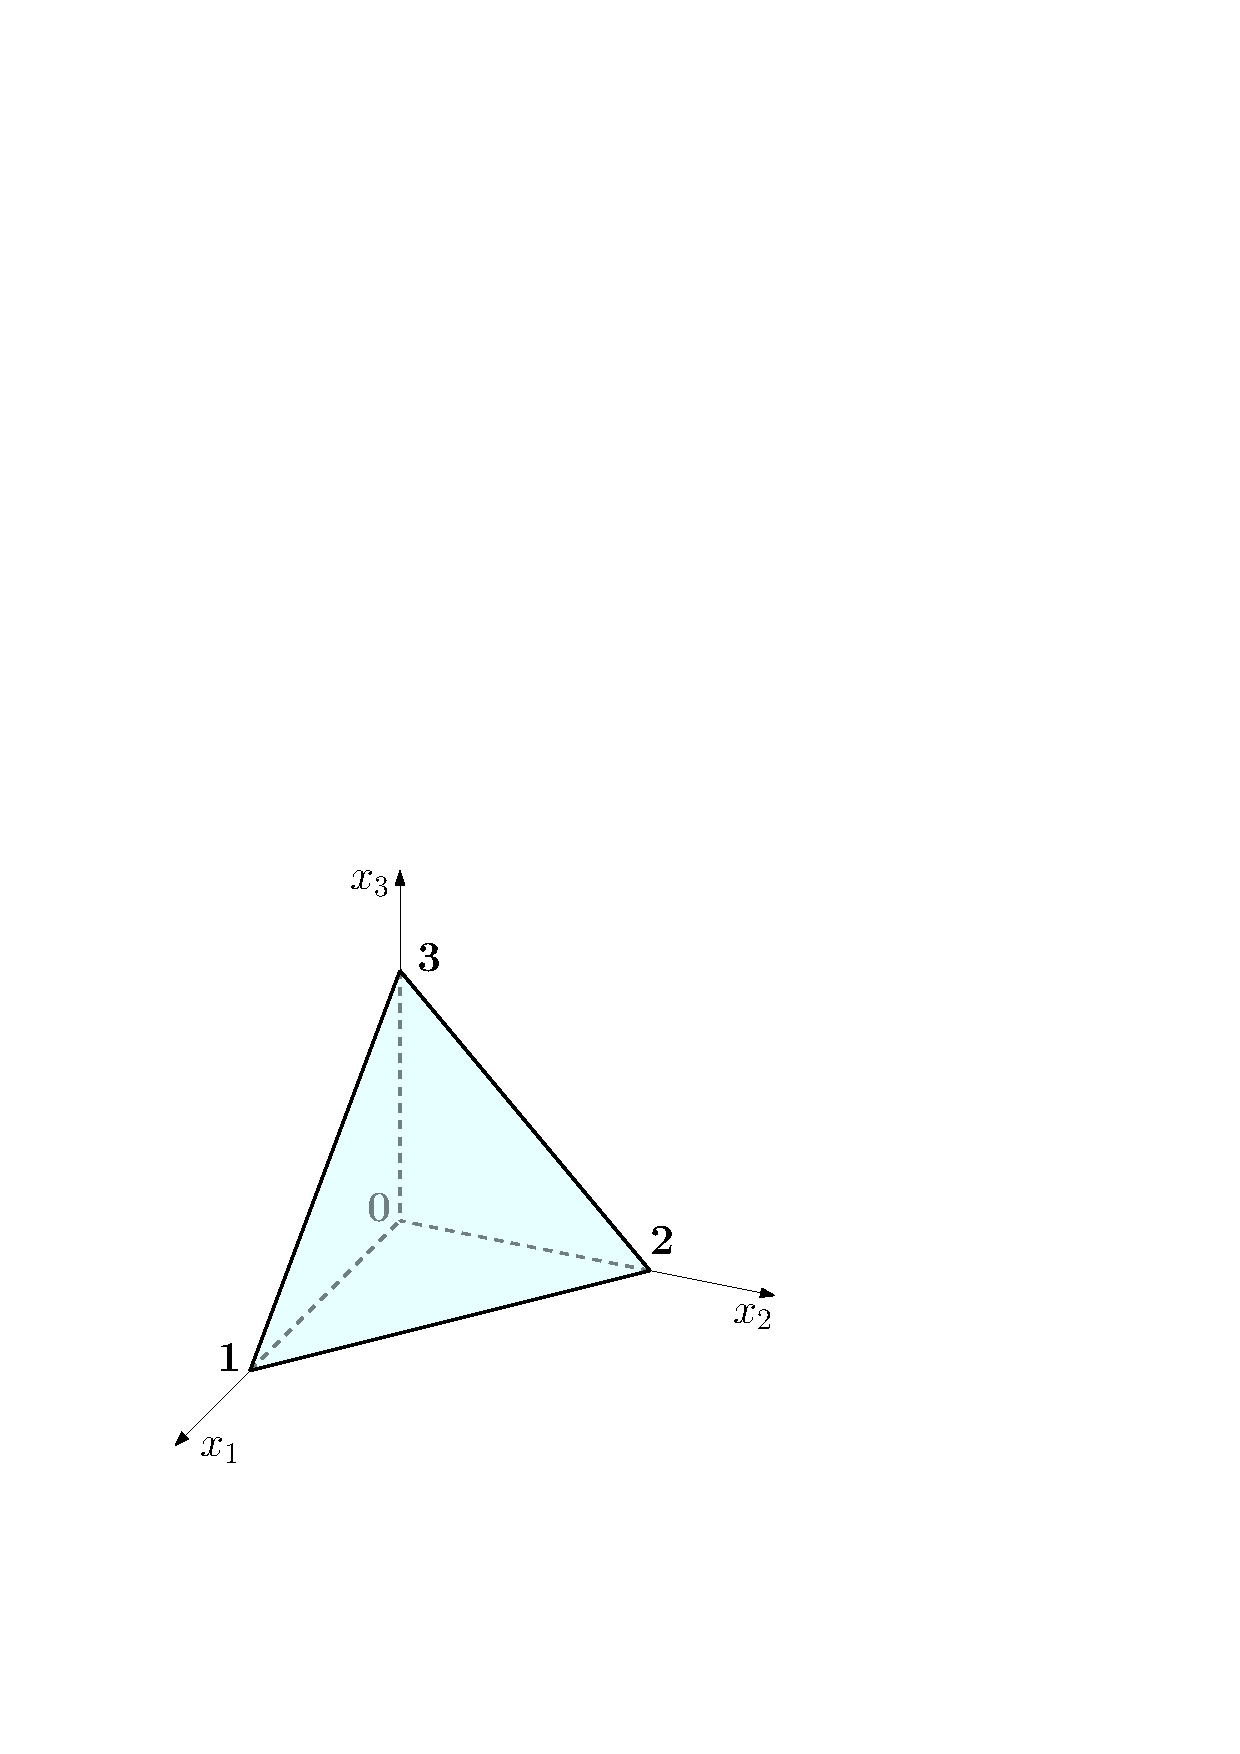
\includegraphics[scale=0.5]{./figures/MasterTet.pdf}
	\end{center}
\end{minipage}} &\\
\multicolumn{3}{|c|}{Affine Coordinates} &\\
\multicolumn{3}{|c|}{
$	\begin{alignedat}{8}
		\lambda_0&=1-x_1-x_2-x_3\qquad\quad&&\phantom{\nabla}\lambda_1&&=x_1\qquad\quad
			&&\phantom{\nabla}\lambda_2&&=x_2\qquad\quad&&\phantom{\nabla}\lambda_3&&=x_3\\
		\nabla\lambda_0&=\bigg(\begin{smallmatrix}-1\\[2pt]-1\\[2pt]-1\end{smallmatrix}\bigg)\qquad\quad 
			&&\nabla\lambda_1&&=\bigg(\begin{smallmatrix}1\\[2pt]0\\[2pt]0\end{smallmatrix}\bigg)\qquad\quad 
				&&\nabla\lambda_2&&=\bigg(\begin{smallmatrix}0\\[2pt]1\\[2pt]0\end{smallmatrix}\bigg)\qquad\quad
					&&\nabla\lambda_3&&=\bigg(\begin{smallmatrix}0\\[2pt]0\\[2pt]1\end{smallmatrix}\bigg)
	\end{alignedat}$} &\\
\multicolumn{3}{|c|}{} &\\[-8pt]
\multicolumn{3}{|c|}{\small\fbox{The order in the quadruple $\vec{\lambda}_{0123}=(\lambda_0,\lambda_1,\lambda_2,\lambda_3)$ and all its subtuples is $p$.}} &\\[-5pt]
{}& {} &{} &\\[-5pt]
\multicolumn{3}{r}{\footnotesize\textit{continued on next page}} &\\[-18.5pt]
\hline
\end{tabular}
\end{center}
\renewcommand{\arraystretch}{1}%Back to normal spacing

\newpage

%%%%%%%%%%%%%%%%%%%%%Tetrahedron 2: H1%%%%%%%%%%%%%%%%%%%%%
\renewcommand{\arraystretch}{1.35}%Better row spacing
\begin{center}
\begin{tabular}
{|C{0.35cm} L{11.9cm}|C{2.9cm}|N}%See main file for this custom columns - they keep a fixed width while maintaining aligment
\multicolumn{3}{l}{\footnotesize\textit{continued from previous page}} &\\[-2pt]
\hline
\multicolumn{3}{|c|}{\large \textbf{Tetrahedron}} &\\
\hline
\multicolumn{3}{|c|}{$H^1$} &\\
\hline
{}& {} &{} &\\[-23pt]%To keep total width fixed
\multicolumn{2}{|c|}{Shape Functions}& Indices &\\ 
\hline
\multicolumn{2}{|l|}{Vertices} &
\multirow{2}{*}[-12pt]{\small$\begin{gathered}
	a\!=\!0,1,2,3
\end{gathered}$} &\\
\multicolumn{2}{|l|}{
$	\begin{aligned}
		\phi^\mathrm{v}&=\lambda_a\\
		\nabla\phi^\mathrm{v}&=\nabla\lambda_a
	\end{aligned}$} &{}&\\
\multicolumn{2}{|l|}{Edges} &
\multirow{2}{*}[-12pt]{\small$\begin{gathered}
	i\!=\!2,\ldots,p\\
	0\leq a<b\leq3
\end{gathered}$} &\\
\multicolumn{2}{|l|}{
$	\begin{aligned}
		\phi_i^\mathrm{e}&=\phi_i^\E(\vec{\lambda}_{ab})\\
		\nabla\phi_i^\mathrm{e}&=\nabla\phi_i^\E(\vec{\lambda}_{ab})
	\end{aligned}$} &{}&\\
\multicolumn{2}{|l|}{Faces} &
\multirow{2}{*}[-12pt]{\small$\begin{gathered}
	i\geq2,\,j\geq1\\
	i\!+\!j\!=\!3,\ldots,p\\
	0\leq a<b<c\leq3	
\end{gathered}$} &\\
\multicolumn{2}{|l|}{
$	\begin{aligned}
		\phi_{ij}^\mathrm{f}&=\phi_{ij}^\Tri(\vec{\lambda}_{abc})\\
		\nabla\phi_{ij}^\mathrm{f}&=\nabla\phi_{ij}^\Tri(\vec{\lambda}_{abc})
	\end{aligned}$} &{}&\\
\multicolumn{2}{|l|}{Interior} &
\multirow{2}{*}[-12pt]{\small$\begin{gathered}
	i\geq2,\,j\geq1,\,k\geq1\\
	i\!+\!j\!+\!k\!=\!4,\ldots,p
\end{gathered}$} &\\[-5pt]
\multicolumn{2}{|l|}{
$	\begin{aligned}
		\phi_{ijk}^\mathrm{b}&=\phi_{ij}^\Tri(\vec{\lambda}_{012})[L_k^{2(i+j)}](1\!-\!\lambda_3,\lambda_3)\\
		\nabla\phi_{ijk}^\mathrm{b}&=
			[L_k^{2(i+j)}](1\!-\!\lambda_3,\lambda_3)\nabla\phi_{ij}^\Tri(\vec{\lambda}_{012})
				+\phi_{ij}^\Tri(\vec{\lambda}_{012})\nabla[L_k^{2(i+j)}](1\!-\!\lambda_3,\lambda_3)
	\end{aligned}$} &{}&\\[-15pt]
{}& {} &{} &\\[-5pt]
\multicolumn{3}{r}{\footnotesize\textit{continued on next page}} &\\[-18.5pt]
\hline
\end{tabular}
\end{center}
\renewcommand{\arraystretch}{1}%Back to normal spacing

\newpage

%%%%%%%%%%%%%%%%%%%%%Tetrahedron 3: Hcurl%%%%%%%%%%%%%%%%%%%%%
\renewcommand{\arraystretch}{1.35}%Better row spacing
\begin{center}
\begin{tabular}
{|C{0.35cm} L{11.9cm}|C{2.9cm}|N}%See main file for this custom columns - they keep a fixed width while maintaining aligment
\multicolumn{3}{l}{\footnotesize\textit{continued from previous page}} &\\[-2pt]
\hline
\multicolumn{3}{|c|}{\large \textbf{Tetrahedron}} &\\
\hline
\multicolumn{3}{|c|}{$H(\mathrm{curl})$} &\\
\hline
{}& {} &{} &\\[-23pt]%To keep total width fixed
\multicolumn{2}{|c|}{Shape Functions}& Indices &\\ 
\hline
\multicolumn{2}{|l|}{Edges} &
\multirow{2}{*}[-12pt]{\small$\begin{gathered}
	i\!=\!0,\ldots,p\!-\!1\\
	0\leq a<b\leq3
\end{gathered}$} &\\
\multicolumn{2}{|l|}{
$	\begin{aligned}
		E_i^\mathrm{e}&=E_i^\E(\vec{\lambda}_{ab})\\
		\nabla\!\times\! E_i^\mathrm{e}&=\nabla\times E_i^\E(\vec{\lambda}_{ab})
	\end{aligned}$} &{}&\\
\multicolumn{2}{|l|}{Faces} & {}&\\[-5pt]
\multicolumn{2}{|l|}{\small $\,$Family I} &
\multirow{2}{*}[-12pt]{\small$\begin{gathered}
	i\geq0,\,j\geq1\\[-2pt]
	i\!+\!j\!=\!1,\ldots,p\!-\!1\\[-2pt]
	0\leq a<b<c\leq3
\end{gathered}$} &\\
\multicolumn{2}{|l|}{
$	\begin{aligned}
		E_{ij}^{\mathrm{f}}&=E_{ij}^\Tri(\vec{\lambda}_{abc})\\
		\nabla\!\times\! E_{ij}^{\mathrm{f}}&=\nabla\!\times\!E_{ij}^\Tri(\vec{\lambda}_{abc})
	\end{aligned}$} &{}&\\
\multicolumn{2}{|l|}{\small $\,$Family II} &
\multirow{2}{*}[-12pt]{\small$\begin{gathered}
	i\geq0,\,j\geq1\\[-2pt]
	i\!+\!j\!=\!1,\ldots,p\!-\!1\\[-2pt]
	0\leq a<b<c\leq3
\end{gathered}$} &\\
\multicolumn{2}{|l|}{
$	\begin{aligned}
		E_{ij}^{\mathrm{f}}&=E_{ij}^\Tri(\vec{\lambda}_{bca})\\
		\nabla\!\times\! E_{ij}^{\mathrm{f}}&=\nabla\!\times\!E_{ij}^\Tri(\vec{\lambda}_{bca})
	\end{aligned}$} &{}&\\
\multicolumn{2}{|l|}{Interior} & {}&\\[-10pt]
\multicolumn{2}{|l|}{\small $\,$Family I} &
\multirow{2}{*}[-12pt]{\small$\begin{gathered}
	i\geq0,\,j\geq1,\,k\geq1\\
	i\!\!+\!\!j\!\!+\!\!k\!=\!2,\ldots,p\!\!-\!\!1
\end{gathered}$} &\\[-5pt]
\multicolumn{2}{|l|}{
$	\begin{aligned}
		E_{ijk}^\mathrm{b}&=[L_k^{2(i+j)}](1\!\!-\!\!\lambda_3,\lambda_3)E_{ij}^\Tri(\vec{\lambda}_{012})\\
		\nabla\!\times\! E_{ijk}^\mathrm{b}&=[L_k^{2(i+j)}](1\!\!-\!\!\lambda_3,\lambda_3)
			\nabla\!\!\times\!\! E_{ij}^\Tri(\vec{\lambda}_{012})
				\!+\!\nabla[L_k^{2(i+j)}](1\!\!-\!\!\lambda_3,\lambda_3)\!\times\! E_{ij}^\Tri(\vec{\lambda}_{012})
	\end{aligned}$} &{}&\\
\multicolumn{2}{|l|}{\small $\,$Family II} &
\multirow{2}{*}[-12pt]{\small$\begin{gathered}
	i\geq0,\,j\geq1,\,k\geq1\\
	i\!\!+\!\!j\!\!+\!\!k\!=\!2,\ldots,p\!\!-\!\!1
\end{gathered}$} &\\[-5pt]
\multicolumn{2}{|l|}{
$	\begin{aligned}
		E_{ijk}^\mathrm{b}&=[L_k^{2(i+j)}](1\!\!-\!\!\lambda_0,\lambda_0)E_{ij}^\Tri(\vec{\lambda}_{123})\\
		\nabla\!\times\! E_{ijk}^\mathrm{b}&=[L_k^{2(i+j)}](1\!\!-\!\!\lambda_0,\lambda_0)
			\nabla\!\!\times\!\! E_{ij}^\Tri(\vec{\lambda}_{123})
				\!+\!\nabla[L_k^{2(i+j)}](1\!\!-\!\!\lambda_0,\lambda_0)\!\times\! E_{ij}^\Tri(\vec{\lambda}_{123})	
	\end{aligned}$} &{}&\\
\multicolumn{2}{|l|}{\small $\,$Family III} &
\multirow{2}{*}[-12pt]{\small$\begin{gathered}
	i\geq0,\,j\geq1,\,k\geq1\\
	i\!\!+\!\!j\!\!+\!\!k\!=\!2,\ldots,p\!\!-\!\!1
\end{gathered}$} &\\[-5pt]
\multicolumn{2}{|l|}{
$	\begin{aligned}
		E_{ijk}^\mathrm{b}&=[L_k^{2(i+j)}](1\!\!-\!\!\lambda_1,\lambda_1)E_{ij}^\Tri(\vec{\lambda}_{230})\\
		\nabla\!\times\! E_{ijk}^\mathrm{b}&=[L_k^{2(i+j)}](1\!\!-\!\!\lambda_1,\lambda_1)
			\nabla\!\!\times\!\! E_{ij}^\Tri(\vec{\lambda}_{230})
				\!+\!\nabla[L_k^{2(i+j)}](1\!\!-\!\!\lambda_1,\lambda_1)\!\times\! E_{ij}^\Tri(\vec{\lambda}_{230})
	\end{aligned}$} &{}&\\[-17pt]
{}& {} &{} &\\[-5pt]
\multicolumn{3}{r}{\footnotesize\textit{continued on next page}} &\\[-18.5pt]
\hline
\end{tabular}
\end{center}
\renewcommand{\arraystretch}{1}%Back to normal spacing

\newpage

%%%%%%%%%%%%%%%%%%%%%Tetrahedron 4: Hdiv,L2%%%%%%%%%%%%%%%%%%%%%
\renewcommand{\arraystretch}{1.35}%Better row spacing
\begin{center}
\begin{tabular}
{|C{0.35cm} L{11.9cm}|C{2.9cm}|N}%See main file for this custom columns - they keep a fixed width while maintaining aligment
\multicolumn{3}{l}{\footnotesize\textit{continued from previous page}} &\\[-2pt]
\hline
\multicolumn{3}{|c|}{\large \textbf{Tetrahedron}} &\\
\hline
\multicolumn{3}{|c|}{$H(\mathrm{div})$} &\\
\hline
{}& {} &{} &\\[-23pt]%To keep total width fixed
\multicolumn{2}{|c|}{Shape Functions}& Indices &\\ 
\hline
\multicolumn{2}{|l|}{Faces} & 
\multirow{2}{*}[-12pt]{\small$\begin{gathered}
	i\geq0,\,j\geq0\\[-2pt]
	i\!+\!j\!=\!0,\ldots,p\!-\!1\\[-2pt]
	0\leq a<b<c\leq3
\end{gathered}$} &\\
\multicolumn{2}{|l|}{
$	\begin{aligned}
		V_{ij}^\mathrm{f}&=V_{ij}^\Tri(\vec{\lambda}_{abc})\\
		\nabla\!\cdot\! V_{ij}^\mathrm{f}&=\nabla\!\cdot\! V_{ij}^\Tri(\vec{\lambda}_{abc}(x))
	\end{aligned}$} &{}&\\
\multicolumn{2}{|l|}{Interior} & {}&\\[-10pt]
\multicolumn{2}{|l|}{\small $\,$Family I} &
\multirow{2}{*}[-12pt]{\small$\begin{gathered}
	i\geq0,\,j\geq0,\,k\geq1\\
	i\!\!+\!\!j\!\!+\!\!k\!=\!1,\ldots,p\!\!-\!\!1
\end{gathered}$} &\\[-5pt]
\multicolumn{2}{|l|}{
$	\begin{aligned}
		V_{ijk}^\mathrm{b}&=[L_k^{2(i\!+\!j\!+\!1)}](1\!\!-\!\!\lambda_3,\lambda_3)V_{ij}^\Tri(\vec{\lambda}_{012})\\
		\nabla\!\cdot\! V_{ijk}^\mathrm{b}&=
			[L_k^{2(i\!+\!j\!+\!1)}](1\!\!-\!\!\lambda_3,\lambda_3)\nabla\!\cdot\! V_{ij}^\Tri(\vec{\lambda}_{012})
				\!+\!\nabla[L_k^{2(i\!+\!j\!+\!1)}](1\!\!-\!\!\lambda_3,\lambda_3)\!\cdot\! V_{ij}^\Tri(\vec{\lambda}_{012})
	\end{aligned}$} &{}&\\
\multicolumn{2}{|l|}{\small $\,$Family II} &
\multirow{2}{*}[-12pt]{\small$\begin{gathered}
	i\geq0,\,j\geq0,\,k\geq1\\
	i\!\!+\!\!j\!\!+\!\!k\!=\!1,\ldots,p\!\!-\!\!1
\end{gathered}$} &\\[-5pt]
\multicolumn{2}{|l|}{
$	\begin{aligned}
		V_{ijk}^\mathrm{b}&=[L_k^{2(i\!+\!j\!+\!1)}](1\!\!-\!\!\lambda_0,\lambda_0)V_{ij}^\Tri(\vec{\lambda}_{123})\\
		\nabla\!\cdot\! V_{ijk}^\mathrm{b}&=
			[L_k^{2(i\!+\!j\!+\!1)}](1\!\!-\!\!\lambda_0,\lambda_0)\nabla\!\cdot\! V_{ij}^\Tri(\vec{\lambda}_{123})
				\!+\!\nabla[L_k^{2(i\!+\!j\!+\!1)}](1\!\!-\!\!\lambda_0,\lambda_0)\!\cdot\! V_{ij}^\Tri(\vec{\lambda}_{123})
	\end{aligned}$} &{}&\\
\multicolumn{2}{|l|}{\small $\,$Family III} &
\multirow{2}{*}[-12pt]{\small$\begin{gathered}
	i\geq0,\,j\geq0,\,k\geq1\\
	i\!\!+\!\!j\!\!+\!\!k\!=\!1,\ldots,p\!\!-\!\!1
\end{gathered}$} &\\[-5pt]
\multicolumn{2}{|l|}{
$	\begin{aligned}
		V_{ijk}^\mathrm{b}&=[L_k^{2(i\!+\!j\!+\!1)}](1\!\!-\!\!\lambda_1,\lambda_1)V_{ij}^\Tri(\vec{\lambda}_{230})\\
		\nabla\!\cdot\! V_{ijk}^\mathrm{b}&=
			[L_k^{2(i\!+\!j\!+\!1)}](1\!\!-\!\!\lambda_1,\lambda_1)\nabla\!\cdot\! V_{ij}^\Tri(\vec{\lambda}_{230})
				\!+\!\nabla[L_k^{2(i\!+\!j\!+\!1)}](1\!\!-\!\!\lambda_1,\lambda_1)\!\cdot\! V_{ij}^\Tri(\vec{\lambda}_{230})
	\end{aligned}$} &{}&\\[-17pt]
{}& {} &{} &\\
\hline
\multicolumn{3}{|c|}{$L^2$} &\\
\hline
{}& {} &{} &\\[-23pt]%To keep total width fixed
\multicolumn{2}{|c|}{Shape Functions}& Indices &\\ 
\hline
\multicolumn{2}{|l|}{Interior} &
\multirow{2}{*}[2pt]{\small$\begin{gathered}
	i\geq0,\,j\geq0,\,k\geq0\\
	i\!\!+\!\!j\!\!+\!\!k\!=\!0,\ldots,p\!\!-\!\!1
\end{gathered}$} &\\[-10pt]
\multicolumn{2}{|l|}{
$	\begin{aligned}
		\psi_{ijk}^\mathrm{b}=[P_i](\vec{\lambda}_{01})[P_j^{2i\!+\!1}](\lambda_0\!+\!\lambda_1,\lambda_2)
			[P_k^{2(i\!+\!j\!+\!1)}](1\!-\!\lambda_3,\lambda_3)(\nabla\lambda_1\!\times\!\nabla\lambda_2)\!\cdot\!\nabla\lambda_3
	\end{aligned}$} &{}&\\[-17pt]
{}& {} &{} &\\
\hline
\end{tabular}
\end{center}
\renewcommand{\arraystretch}{1}%Back to normal spacing


\newpage
\subsection{Prism}

%%%%%%%%%%%%%%%%%%%%%Prism 1: Geometry%%%%%%%%%%%%%%%%%%%%%
\renewcommand{\arraystretch}{1.35}%Better row spacing
\begin{center}
\begin{tabular}
{|C{0.35cm} L{11.9cm} C{2.9cm}|N}%See main file for this custom columns - they keep a fixed width while maintaining aligment
\hline
\multicolumn{3}{|c|}{\large \textbf{Prism}} &\\
\hline
\multicolumn{3}{|c|}{Geometry} &\\
\hline
\multicolumn{3}{|c|}{} &\\[-10pt]
\multicolumn{3}{|c|}{\begin{minipage}{0.9\textwidth}
	\begin{center}
		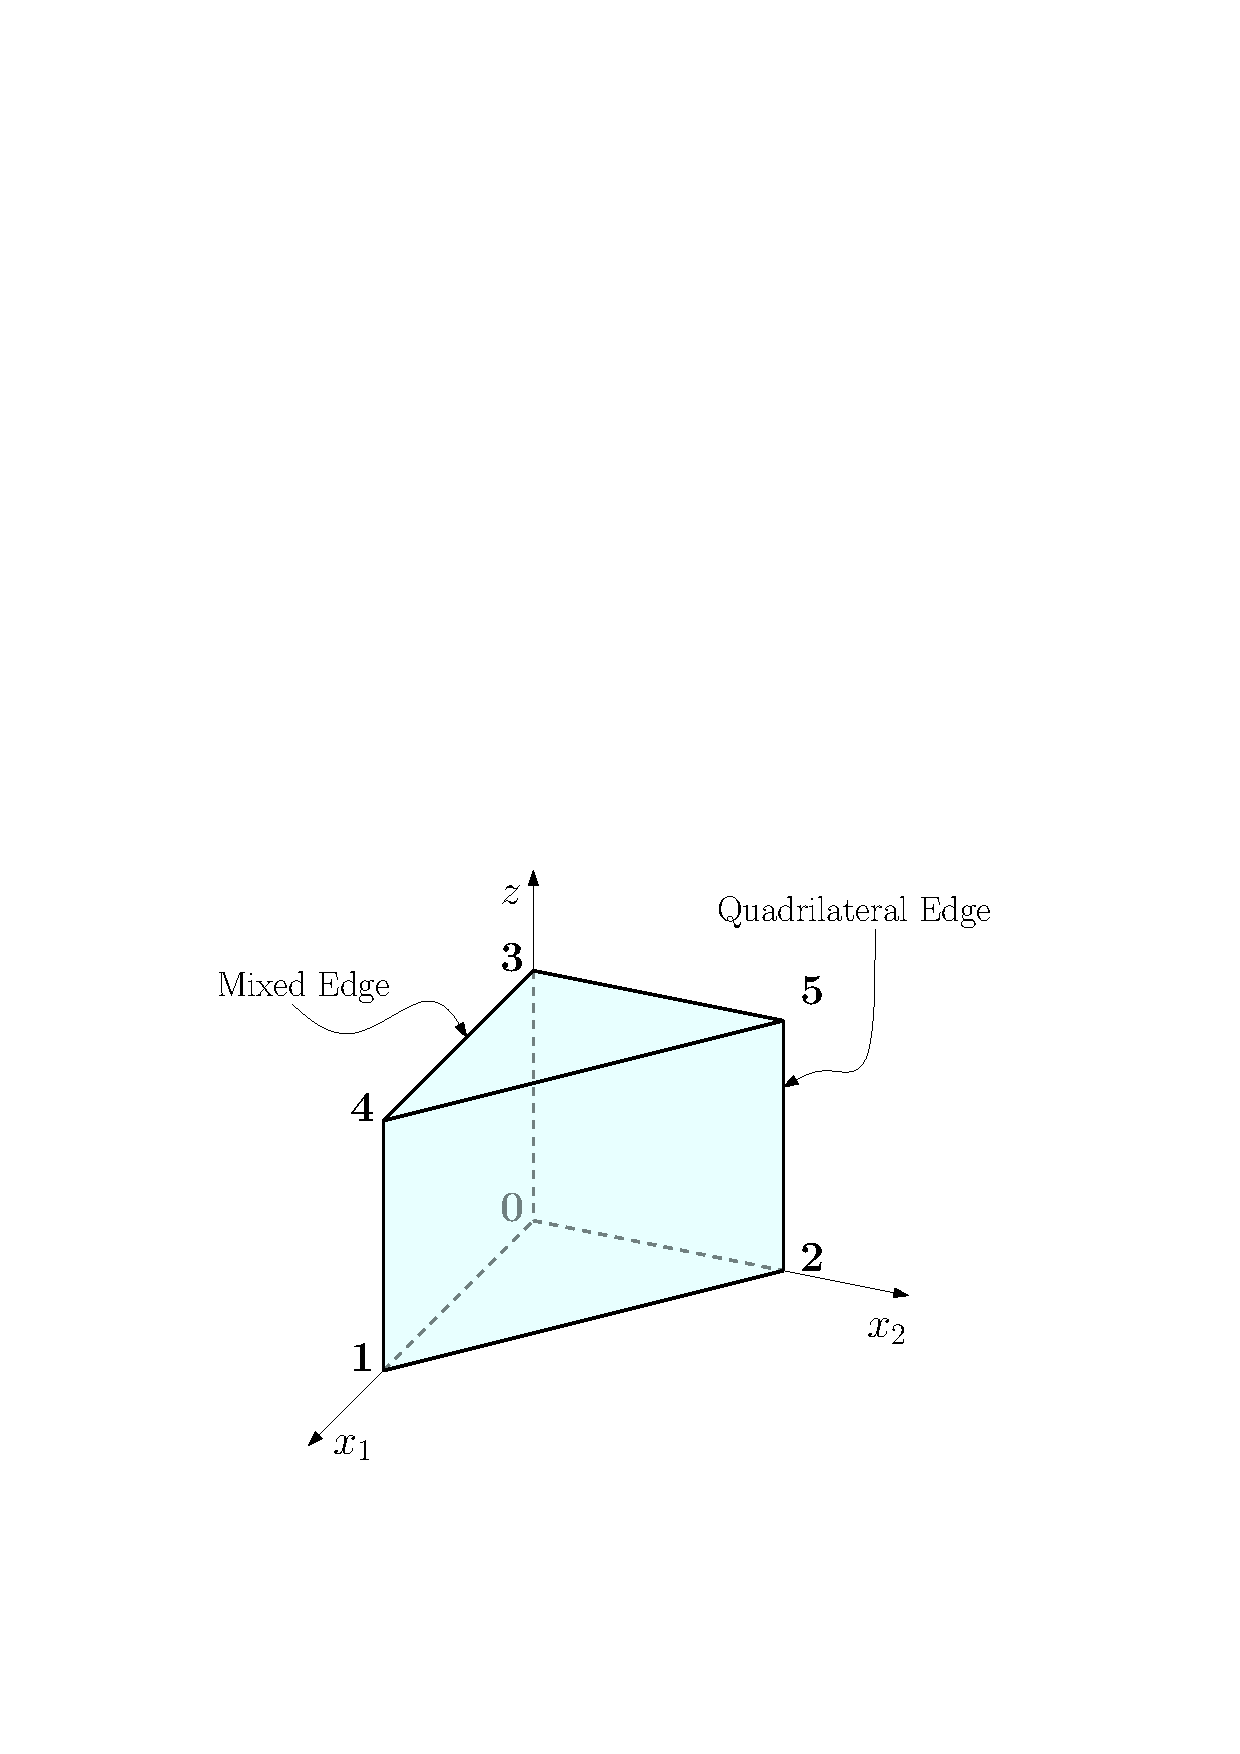
\includegraphics[scale=0.5]{./figures/MasterPrismTables.pdf}
	\end{center}
\end{minipage}} &\\
\multicolumn{3}{|c|}{Affine Coordinates} &\\
\multicolumn{3}{|c|}{
$	\begin{alignedat}{6}
		\nu_0&=1-x_1-x_2\,\qquad\qquad &&\phantom{\nabla}\nu_1&&=x_1\qquad\qquad &&\phantom{\nabla}\nu_2&&=x_2\\
		\nabla\nu_0&=\bigg(\begin{smallmatrix}-1\\[2pt]-1\\[2pt]0\end{smallmatrix}\bigg)\qquad\qquad 
			&&\nabla\nu_1&&=\bigg(\begin{smallmatrix}1\\[2pt]0\\[2pt]0\end{smallmatrix}\bigg)\qquad\qquad 
				&&\nabla\nu_2&&=\bigg(\begin{smallmatrix}0\\[2pt]1\\[2pt]0\end{smallmatrix}\bigg)
	\end{alignedat}$} &\\[30pt]
\multicolumn{3}{|c|}{
$	\begin{alignedat}{4}
		\mu_0&=1-z\,\qquad\qquad &&\phantom{\nabla}\mu_1&&=z\\
		\nabla\mu_0&=\bigg(\begin{smallmatrix}0\\[2pt]0\\[2pt]-1\end{smallmatrix}\bigg)\qquad\qquad 
			&&\nabla\mu_1&&=\bigg(\begin{smallmatrix}0\\[2pt]0\\[2pt]1\end{smallmatrix}\bigg)
	\end{alignedat}$} &\\
\multicolumn{3}{|c|}{} &\\[-8pt]
\multicolumn{3}{|c|}{\small\fbox{\parbox[c][25pt][c]{0.6\textwidth}{The order in the triplet $\vec{\nu}_{012}=(\nu_0,\nu_1,\nu_2)$ and all its subpairs is $p$.\\The order in the pair $\vec{\mu}_{01}=(\mu_0,\mu_1)$ is $q$.}}} &\\
{}& {} &{} &\\[-5pt]
\multicolumn{3}{r}{\footnotesize\textit{continued on next page}} &\\[-18.5pt]
\hline
\end{tabular}
\end{center}
\renewcommand{\arraystretch}{1}%Back to normal spacing

\newpage

%%%%%%%%%%%%%%%%%%%%%Prism 2: H1%%%%%%%%%%%%%%%%%%%%%
\renewcommand{\arraystretch}{1.35}%Better row spacing
\begin{center}
\begin{tabular}
{|C{0.35cm} L{11.9cm}|C{2.9cm}|N}%See main file for this custom columns - they keep a fixed width while maintaining aligment
\multicolumn{3}{l}{\footnotesize\textit{continued from previous page}} &\\[-2pt]
\hline
\multicolumn{3}{|c|}{\large \textbf{Prism}} &\\
\hline
\multicolumn{3}{|c|}{$H^1$} &\\
\hline
{}& {} &{} &\\[-23pt]%To keep total width fixed
\multicolumn{2}{|c|}{Shape Functions}& Indices &\\ 
\hline
\multicolumn{2}{|l|}{Vertices} &
\multirow{2}{*}[-12pt]{\small$\begin{gathered}
	a\!=\!0,1,2\\
	c\!=\!0,1
\end{gathered}$} &\\
\multicolumn{2}{|l|}{
$	\begin{aligned}
		\phi^\mathrm{v}&=\nu_a\mu_c\\
		\nabla\phi^\mathrm{v}&=\mu_c\nabla\nu_a+\nu_a\nabla\mu_c
	\end{aligned}$} &{}&\\
\multicolumn{2}{|l|}{Mixed Edges} &
\multirow{2}{*}[-10pt]{\small$\begin{gathered}
	i\!=\!2,\ldots,p\\[-2pt]
	0\leq a<b\leq2\\[-2pt]
	c\!=\!0,1
\end{gathered}$} &\\
\multicolumn{2}{|l|}{
$	\begin{aligned}
		\phi_i^\mathrm{e}&=\mu_c\phi_i^\E(\vec{\nu}_{ab})\\
		\nabla\phi_i^\mathrm{e}&=\mu_c\nabla\phi_i^\E(\vec{\nu}_{ab})+\phi_i^\E(\vec{\nu}_{ab})\nabla\mu_c
	\end{aligned}$} &{}&\\
\multicolumn{2}{|l|}{Quadrilateral Edges} &
\multirow{2}{*}[-10pt]{\small$\begin{gathered}
	i\!=\!2,\ldots,q\\
	a=0,1,2
\end{gathered}$} &\\
\multicolumn{2}{|l|}{
$	\begin{aligned}
		\phi_i^\mathrm{e}&=\nu_a\phi_i^\E(\vec{\mu}_{01})\\
		\nabla\phi_i^\mathrm{e}&=\nu_a\nabla\phi_i^\E(\vec{\mu}_{01})+\phi_i^\E(\vec{\mu}_{01})\nabla\nu_a
	\end{aligned}$} &{}&\\
\multicolumn{2}{|l|}{Triangle Faces} &
\multirow{2}{*}[-12pt]{\small$\begin{gathered}
	i\geq2,\,j\geq1\\[-2pt]
	i\!+\!j\!=\!3,\ldots,p\\[-2pt]
	c\!=\!0,1	
\end{gathered}$} &\\
\multicolumn{2}{|l|}{
$	\begin{aligned}
		\phi_{ij}^\mathrm{f}&=\mu_c\phi_{ij}^\Tri(\vec{\nu}_{012})\\
		\nabla\phi_{ij}^\mathrm{f}&=\mu_c\nabla\phi_{ij}^\Tri(\vec{\nu}_{012})+\phi_{ij}^\Tri(\vec{\nu}_{012})\nabla\mu_c
	\end{aligned}$} &{}&\\
\multicolumn{2}{|l|}{Quadrilateral Faces} &
\multirow{2}{*}[-12pt]{\small$\begin{gathered}
	i\!=\!2,\ldots,p\\[-2pt]
	j\!=\!2,\ldots,q\\[-2pt]
	0\leq a<b\leq2	
\end{gathered}$} &\\
\multicolumn{2}{|l|}{
$	\begin{aligned}
		\phi_{ij}^\mathrm{f}&=\phi_{ij}^\square(\vec{\nu}_{ab},\vec{\mu}_{01})\\
		\nabla\phi_{ij}^\mathrm{f}&=\nabla\phi_{ij}^\square(\vec{\nu}_{ab},\vec{\mu}_{01})
	\end{aligned}$} &{}&\\
\multicolumn{2}{|l|}{Interior} &
\multirow{2}{*}[-12pt]{\small$\begin{gathered}
	i\geq2,\,j\geq1\\[-2pt]
	i\!+\!j\!=\!3,\ldots,p\\[-2pt]
	k\!=\!2,\ldots,q
\end{gathered}$} &\\
\multicolumn{2}{|l|}{
$	\begin{aligned}
		\phi_{ijk}^\mathrm{b}&=\phi_{ij}^\Tri(\vec{\nu}_{012})\phi_k^\E(\vec{\mu}_{01})\\
		\nabla\phi_{ijk}^\mathrm{b}&=\phi_k^\E(\vec{\mu}_{01})\nabla\phi_{ij}^\Tri(\vec{\nu}_{012})
			+\phi_{ij}^\Tri(\vec{\nu}_{012})\nabla\phi_k^\E(\vec{\mu}_{01})
	\end{aligned}$} &{}&\\[-15pt]
{}& {} &{} &\\[-5pt]
\multicolumn{3}{r}{\footnotesize\textit{continued on next page}} &\\[-18.5pt]
\hline
\end{tabular}
\end{center}
\renewcommand{\arraystretch}{1}%Back to normal spacing

\newpage

%%%%%%%%%%%%%%%%%%%%%Prism 3: Hcurl%%%%%%%%%%%%%%%%%%%%%
\renewcommand{\arraystretch}{1.35}%Better row spacing
\begin{center}
\begin{tabular}
{|C{0.35cm} L{11.9cm}|C{2.9cm}|N}%See main file for this custom columns - they keep a fixed width while maintaining aligment
\multicolumn{3}{l}{\footnotesize\textit{continued from previous page}} &\\[-2pt]
\hline
\multicolumn{3}{|c|}{\large \textbf{Prism}} &\\
\hline
\multicolumn{3}{|c|}{$H(\mathrm{curl})$} &\\
\hline
{}& {} &{} &\\[-23pt]%To keep total width fixed
\multicolumn{2}{|c|}{Shape Functions}& Indices &\\ 
\hline
\multicolumn{2}{|l|}{Mixed Edges} &
\multirow{2}{*}[-10pt]{\small$\begin{gathered}
	i\!=\!0,\ldots,p\!-\!1\\[-2pt]
	0\leq a<b\leq2\\[-2pt]
	c\!=\!0,1
\end{gathered}$} &\\
\multicolumn{2}{|l|}{
$	\begin{aligned}
		E_i^\mathrm{e}&=\mu_cE_i^\E(\vec{\nu}_{ab})\\
		\nabla\!\times\! E_i^\mathrm{e}&=\mu_c\nabla\!\times\! E_i^\E(\vec{\nu}_{ab})+\nabla\mu_c\!\times\! E_i^\E(\vec{\nu}_{ab})
	\end{aligned}$} &{}&\\
\multicolumn{2}{|l|}{Quadrilateral Edges} &
\multirow{2}{*}[-10pt]{\small$\begin{gathered}
	i\!=\!0,\ldots,q\!-\!1\\
	a=0,1,2
\end{gathered}$} &\\
\multicolumn{2}{|l|}{
$	\begin{aligned}
		E_i^\mathrm{e}&=\nu_aE_i^\E(\vec{\mu}_{01})\\
		\nabla\!\times\! E_i^\mathrm{e}&=\nabla\nu_a\!\times\! E_i^\E(\vec{\mu}_{01})
	\end{aligned}$} &{}&\\
\multicolumn{2}{|l|}{Triangle Faces} & {}&\\[-5pt]
\multicolumn{2}{|l|}{\small $\,$Family I} &
\multirow{2}{*}[-12pt]{\small$\begin{gathered}
	i\geq0,\,j\geq1\\[-2pt]
	i\!+\!j\!=\!1,\ldots,p\!-\!1\\[-2pt]
	c\!=\!0,1
\end{gathered}$} &\\
\multicolumn{2}{|l|}{
$	\begin{aligned}
		E_{ij}^{\mathrm{f}}&=\mu_cE_{ij}^\Tri(\vec{\nu}_{012})\\
		\nabla\!\times\! E_{ij}^{\mathrm{f}}&=\mu_c\nabla\!\times\! E_{ij}^\Tri(\vec{\nu}_{012})
			+\nabla\mu_c\!\times\! E_{ij}^\Tri(\vec{\nu}_{012})
	\end{aligned}$} &{}&\\
\multicolumn{2}{|l|}{\small $\,$Family II} &
\multirow{2}{*}[-12pt]{\small$\begin{gathered}
	i\geq0,\,j\geq1\\[-2pt]
	i\!+\!j\!=\!1,\ldots,p\!-\!1\\[-2pt]
	c\!=\!0,1
\end{gathered}$} &\\
\multicolumn{2}{|l|}{
$	\begin{aligned}
		E_{ij}^{\mathrm{f}}&=\mu_cE_{ij}^\Tri(\vec{\nu}_{120})\\
		\nabla\!\times\! E_{ij}^{\mathrm{f}}&=\mu_c\nabla\!\times\! E_{ij}^\Tri(\vec{\nu}_{120})
			+\nabla\mu_c\!\times\! E_{ij}^\Tri(\vec{\nu}_{120})
	\end{aligned}$} &{}&\\
\multicolumn{2}{|l|}{Quadrilateral Faces} & {}&\\[-5pt]
\multicolumn{2}{|l|}{\small $\,$Family I} &
\multirow{2}{*}[-12pt]{\small$\begin{gathered}
	i\!=\!0,\ldots,p\!-\!1\\[-2pt]
	j\!=\!2,\ldots,q\\[-2pt]
	0\leq a<b\leq2
\end{gathered}$} &\\
\multicolumn{2}{|l|}{
$	\begin{aligned}
		E_{ij}^{\mathrm{f}}&=E_{ij}^\square(\vec{\nu}_{ab},\vec{\mu}_{01})\\
		\nabla\!\times\! E_{ij}^{\mathrm{f}}&=\nabla\!\times\! E_{ij}^\square(\vec{\nu}_{ab},\vec{\mu}_{01})
	\end{aligned}$} &{}&\\
\multicolumn{2}{|l|}{\small $\,$Family II} &
\multirow{2}{*}[-12pt]{\small$\begin{gathered}
	i\!=\!0,\ldots,q\!-\!1\\[-2pt]
	j\!=\!2,\ldots,p\\[-2pt]
	0\leq a<b\leq2
\end{gathered}$} &\\
\multicolumn{2}{|l|}{
$	\begin{aligned}
		E_{ij}^{\mathrm{f}}&=E_{ij}^\square(\vec{\mu}_{01},\vec{\nu}_{ab})\\
		\nabla\!\times\! E_{ij}^{\mathrm{f}}&=\nabla\!\times\! E_{ij}^\square(\vec{\mu}_{01},\vec{\nu}_{ab})
	\end{aligned}$} &{}&\\[-13pt]
{}& {} &{} &\\[-5pt]
\multicolumn{3}{r}{\footnotesize\textit{continued on next page}} &\\[-18.5pt]
\hline
\end{tabular}
\end{center}
\renewcommand{\arraystretch}{1}%Back to normal spacing

\newpage

%%%%%%%%%%%%%%%%%%%%%Prism 4: Hcurl Interior%%%%%%%%%%%%%%%%%%%%%
\renewcommand{\arraystretch}{1.35}%Better row spacing
\begin{center}
\begin{tabular}
{|C{0.35cm} L{11.9cm}|C{2.9cm}|N}%See main file for this custom columns - they keep a fixed width while maintaining aligment
\multicolumn{3}{l}{\footnotesize\textit{continued from previous page}} &\\[-2pt]
\hline
\multicolumn{3}{|c|}{\large \textbf{Prism}} &\\
\hline
\multicolumn{3}{|c|}{$H(\mathrm{curl})$} &\\
\hline
{}& {} &{} &\\[-23pt]%To keep total width fixed
\multicolumn{2}{|c|}{Shape Functions}& Indices &\\ 
\hline
\multicolumn{2}{|l|}{Interior} & {}&\\[-5pt]
\multicolumn{2}{|l|}{\small $\,$Family I} &
\multirow{2}{*}[-12pt]{\small$\begin{gathered}
	i\geq0,\,j\geq1\\[-2pt]
	i\!+\!j\!=\!1,\ldots,p\!-\!1\\[-2pt]
	k\!=\!2,\ldots,q
\end{gathered}$} &\\
\multicolumn{2}{|l|}{
$	\begin{aligned}
		E_{ijk}^\mathrm{b}&=\phi_k^\E(\vec{\mu}_{01})E_{ij}^\Tri(\vec{\nu}_{012})\\
		\nabla\!\times\! E_{ijk}^\mathrm{b}&=\phi_k^\E(\vec{\mu}_{01})\nabla\!\times\! E_{ij}^\Tri(\vec{\nu}_{012})
			+\nabla\phi_k^\E(\vec{\mu}_{01})\!\times\! E_{ij}^\Tri(\vec{\nu}_{012})
	\end{aligned}$} &{}&\\
\multicolumn{2}{|l|}{\small $\,$Family II} &
\multirow{2}{*}[-12pt]{\small$\begin{gathered}
	i\geq0,\,j\geq1\\[-2pt]
	i\!+\!j\!=\!1,\ldots,p\!-\!1\\[-2pt]
	k\!=\!2,\ldots,q
\end{gathered}$} &\\
\multicolumn{2}{|l|}{
$	\begin{aligned}
		E_{ijk}^\mathrm{b}&=\phi_k^\E(\vec{\mu}_{01})E_{ij}^\Tri(\vec{\nu}_{120})\\
		\nabla\!\times\! E_{ijk}^\mathrm{b}&=\phi_k^\E(\vec{\mu}_{01})\nabla\!\times\! E_{ij}^\Tri(\vec{\nu}_{120})
			+\nabla\phi_k^\E(\vec{\mu}_{01})\!\times\! E_{ij}^\Tri(\vec{\nu}_{120})
	\end{aligned}$} &{}&\\
\multicolumn{2}{|l|}{\small $\,$Family III} &
\multirow{2}{*}[-12pt]{\small$\begin{gathered}
	i\geq2,\,j\geq1\\[-2pt]
	i\!+\!j\!=\!3,\ldots,p\\[-2pt]
	k\!=\!0,\ldots,q\!-\!1
\end{gathered}$} &\\
\multicolumn{2}{|l|}{
$	\begin{aligned}
		E_{ijk}^\mathrm{b}&=\phi_{ij}^\Tri(\vec{\nu}_{012})E_k^\E(\vec{\mu}_{01})\\
		\nabla\!\times\! E_{ijk}^\mathrm{b}&=\nabla\phi_{ij}^\Tri(\vec{\nu}_{012})\!\times\! E_k^\E(\vec{\mu}_{01})
	\end{aligned}$} &{}&\\[-17pt]
{}& {} &{} &\\[-5pt]
\multicolumn{3}{r}{\footnotesize\textit{continued on next page}} &\\[-18.5pt]
\hline
\end{tabular}
\end{center}
\renewcommand{\arraystretch}{1}%Back to normal spacing

\newpage

%%%%%%%%%%%%%%%%%%%%%Prism 5: Hdiv,L2%%%%%%%%%%%%%%%%%%%%%
\renewcommand{\arraystretch}{1.35}%Better row spacing
\begin{center}
\begin{tabular}
{|C{0.35cm} L{11.9cm}|C{2.9cm}|N}%See main file for this custom columns - they keep a fixed width while maintaining aligment
\multicolumn{3}{l}{\footnotesize\textit{continued from previous page}} &\\[-2pt]
\hline
\multicolumn{3}{|c|}{\large \textbf{Prism}} &\\
\hline
\multicolumn{3}{|c|}{$H(\mathrm{div})$} &\\
\hline
{}& {} &{} &\\[-23pt]%To keep total width fixed
\multicolumn{2}{|c|}{Shape Functions}& Indices &\\ 
\hline
\multicolumn{2}{|l|}{Triangle Faces} & 
\multirow{2}{*}[-12pt]{\small$\begin{gathered}
	i\geq0,\,j\geq0\\[-2pt]
	i\!+\!j\!=\!0,\ldots,p\!-\!1\\[-2pt]
	c\!=\!0,1
\end{gathered}$} &\\
\multicolumn{2}{|l|}{
$	\begin{aligned}
		V_{ij}^\mathrm{f}&=\mu_cV_{ij}^\Tri(\vec{\nu}_{012})\\
		\nabla\!\cdot\! V_{ij}^\mathrm{f}&=\nabla\mu_c\!\cdot\! V_{ij}^\Tri(\vec{\nu}_{012})
	\end{aligned}$} &{}&\\
\multicolumn{2}{|l|}{Quadrilateral Faces} & 
\multirow{2}{*}[-12pt]{\small$\begin{gathered}
	i\!=\!0,\ldots,p\!-\!1\\[-2pt]
	j\!=\!0,\ldots,q\!-\!1\\[-2pt]
	0\leq a<b\leq2
\end{gathered}$} &\\
\multicolumn{2}{|l|}{
$	\begin{aligned}
		V_{ij}^\mathrm{f}&=V_{ij}^\square(\vec{\nu}_{ab},\vec{\mu}_{01})\\
		\nabla\!\cdot\! V_{ij}^\mathrm{f}&=\nabla\!\cdot\! V_{ij}^\square(\vec{\nu}_{ab},\vec{\mu}_{01})
	\end{aligned}$} &{}&\\
\multicolumn{2}{|l|}{Interior} & {}&\\[-5pt]
\multicolumn{2}{|l|}{\small $\,$Family I} &
\multirow{2}{*}[-12pt]{\small$\begin{gathered}
	i\geq0,\,j\geq1\\[-2pt]
	i\!+\!j\!=\!1,\ldots,p\!-\!1\\[-2pt]
	k\!=\!0,\ldots,q\!-\!1
\end{gathered}$} &\\
\multicolumn{2}{|l|}{
$	\begin{aligned}
		V_{ijk}^\mathrm{b}&=E_{ij}^\Tri(\vec{\nu}_{012})\!\times\! E_k^\E(\vec{\mu}_{01})\\
		\nabla\!\cdot\! V_{ijk}^\mathrm{b}&=E_k^\E(\vec{\mu}_{01})\cdot\Big(\nabla\!\times\! E_{ij}^\Tri(\vec{\nu}_{012})\Big)
	\end{aligned}$} &{}&\\
\multicolumn{2}{|l|}{\small $\,$Family II} &
\multirow{2}{*}[-12pt]{\small$\begin{gathered}
	i\geq0,\,j\geq1\\[-2pt]
	i\!+\!j\!=\!1,\ldots,p\!-\!1\\[-2pt]
	k\!=\!0,\ldots,q\!-\!1
\end{gathered}$} &\\
\multicolumn{2}{|l|}{
$	\begin{aligned}
		V_{ijk}^\mathrm{b}&=E_{ij}^\Tri(\vec{\nu}_{120})\!\times\! E_k^\E(\vec{\mu}_{01})\\
		\nabla\!\cdot\! V_{ijk}^\mathrm{b}&=E_k^\E(\vec{\mu}_{01})\!\cdot\!\Big(\nabla\!\times\! E_{ij}^\Tri(\vec{\nu}_{120})\Big)
	\end{aligned}$} &{}&\\
\multicolumn{2}{|l|}{\small $\,$Family III} &
\multirow{2}{*}[-12pt]{\small$\begin{gathered}
	i\geq0,\,j\geq0\\[-2pt]
	i\!+\!j\!=\!0,\ldots,p\!-\!1\\[-2pt]
	k\!=\!2,\ldots,q
\end{gathered}$} &\\
\multicolumn{2}{|l|}{
$	\begin{aligned}
		V_{ijk}^\mathrm{b}&=\phi_k^\E(\vec{\mu}_{01})V_{ij}^\Tri(\vec{\nu}_{012})\\
		\nabla\!\cdot\! V_{ijk}^\mathrm{b}&=\nabla\phi_k^\E(\vec{\mu}_{01})\!\cdot\! V_{ij}^\Tri(\vec{\nu}_{012})
	\end{aligned}$} &{}&\\[-17pt]
{}& {} &{} &\\
\hline
\multicolumn{3}{|c|}{$L^2$} &\\
\hline
{}& {} &{} &\\[-23pt]%To keep total width fixed
\multicolumn{2}{|c|}{Shape Functions}& Indices &\\ 
\hline
\multicolumn{2}{|l|}{Interior} &
\multirow{2}{*}[-7pt]{\small$\begin{gathered}
	i\geq0,\,j\geq0\\[-2pt]
	i\!+\!j\!=\!0,\ldots,p\!-\!1\\[-2pt]
	k\!=\!0,\ldots,q\!-\!1
\end{gathered}$} &\\
\multicolumn{2}{|l|}{
$	\begin{aligned}
		\psi_{ijk}^\mathrm{b}=[P_i](\vec{\nu}_{01})[P_j^{2i+1}](\nu_0+\nu_1,\nu_2)[P_k](\vec{\mu}_{01})
			(\nabla\nu_1\!\times\!\nabla\nu_2)\!\cdot\!\nabla\mu_1
	\end{aligned}$} &{}&\\[-10pt]
{}& {} &{} &\\
\hline
\end{tabular}
\end{center}
\renewcommand{\arraystretch}{1}%Back to normal spacing



\newpage
\subsection{Pyramid}

%%%%%%%%%%%%%%%%%%%%%Pyramid 1: Geometry%%%%%%%%%%%%%%%%%%%%%
\renewcommand{\arraystretch}{1.35}%Better row spacing
\begin{center}
\begin{tabular}
{|C{0.35cm} L{11.9cm} C{2.9cm}|N}%See main file for this custom columns - they keep a fixed width while maintaining aligment
\hline
\multicolumn{3}{|c|}{\large \textbf{Pyramid}} &\\
\hline
\multicolumn{3}{|c|}{Geometry} &\\
\hline
\multicolumn{3}{|c|}{} &\\[-10pt]
\multicolumn{3}{|c|}{\begin{minipage}{0.4\textwidth}
	\begin{center}
		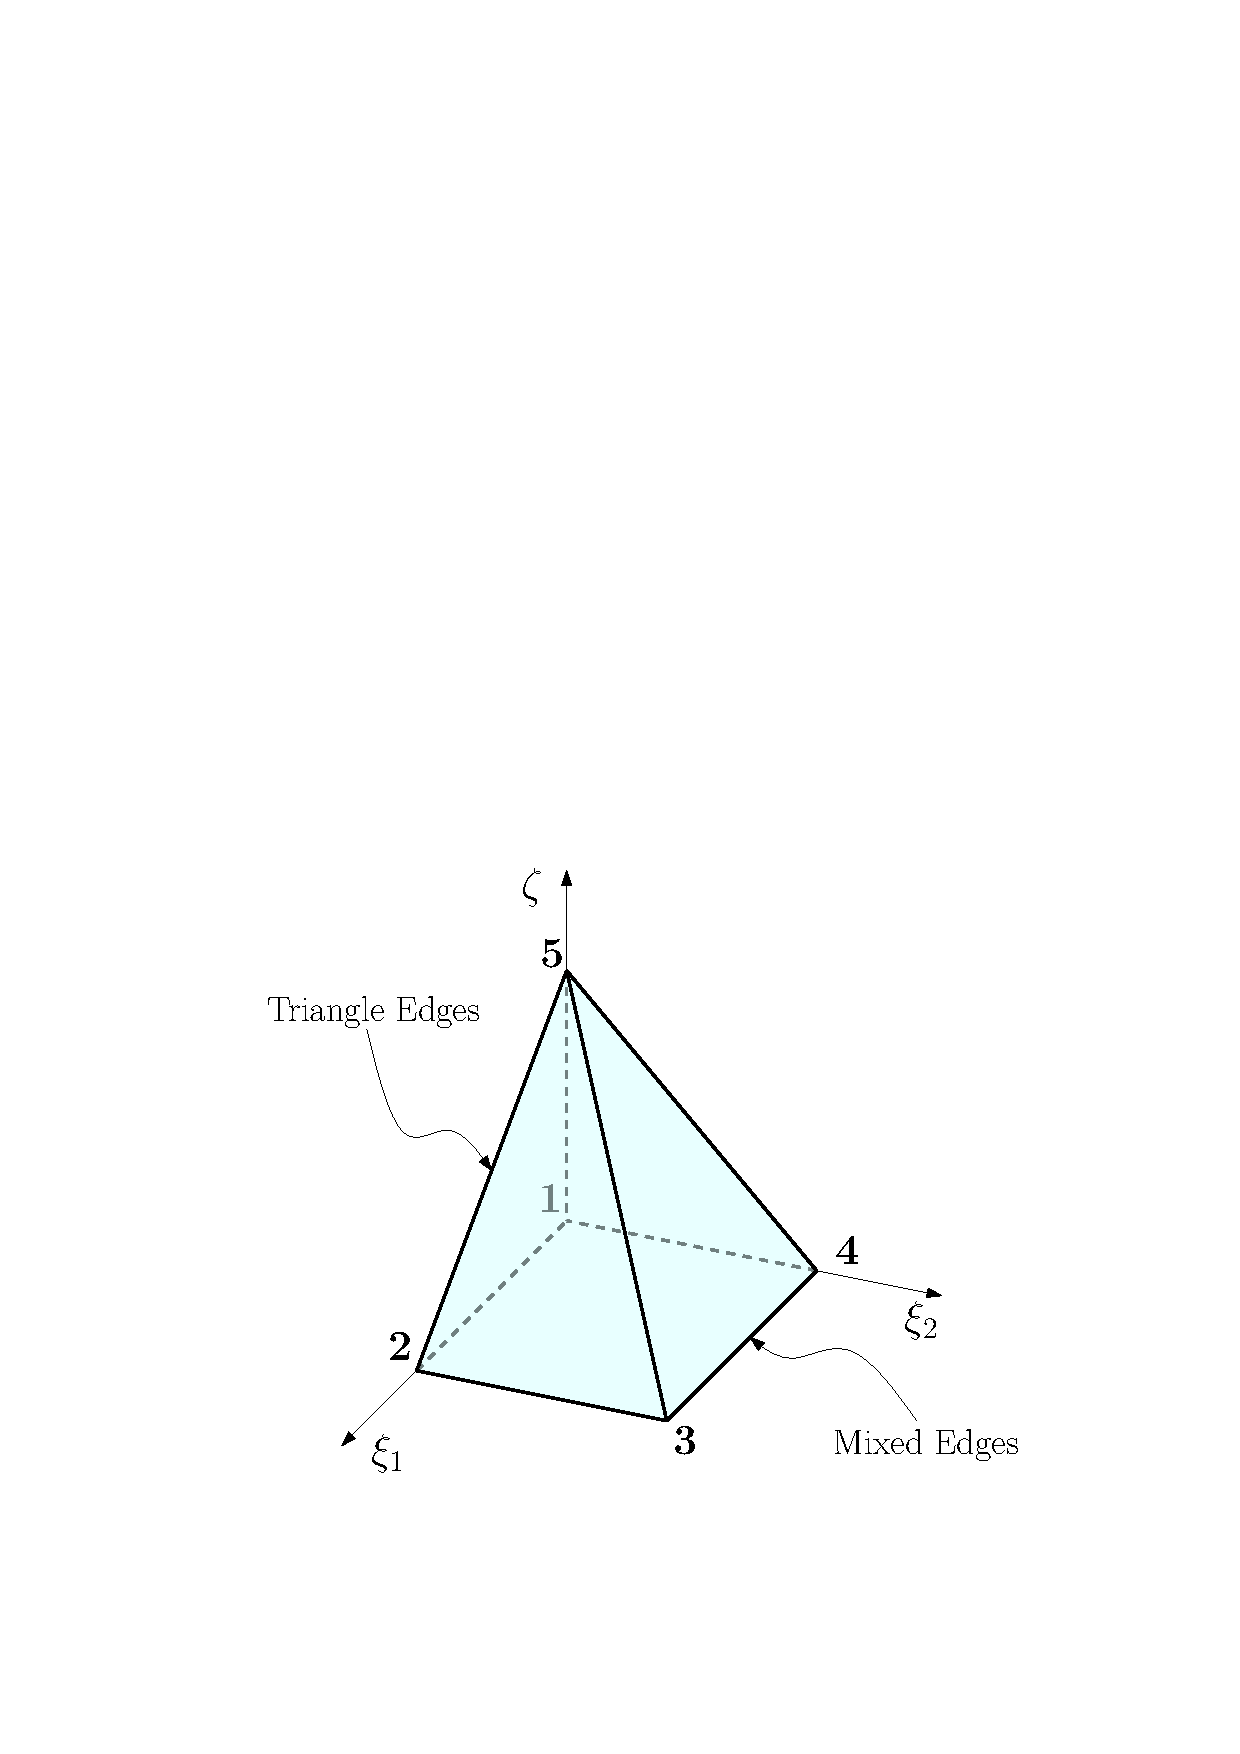
\includegraphics[scale=0.5]{./figures/MasterPyramidTables.pdf}
	\end{center}
\end{minipage}
\begin{minipage}{0.55\textwidth}
	\begin{center}
		Affine Coordinates
		$	\begin{alignedat}{4}
		{}&{}&&{}&&{}\\[-7pt]
		\mu_0^{\,\zeta,\xi_1}&=1-\sxi\,\quad &&\phantom{\nabla}\mu_1^{\,\zeta,\xi_1}&&=\sxi\\
		\nabla\mu_0^{\,\zeta,\xi_1}&=
			\textstyle{\frac{1}{(1-\zeta)^2}}\bigg(\begin{smallmatrix}-(1-\zeta)\\[2pt]0\\[2pt]-\xi_1\end{smallmatrix}\bigg)\quad 
				&&\nabla\mu_1^{\,\zeta,\xi_1}&&=
					\textstyle{\frac{1}{(1-\zeta)^2}}\bigg(\begin{smallmatrix}(1-\zeta)\\[2pt]0\\[2pt]\xi_1\end{smallmatrix}\bigg)\\
		\mu_0^{\,\zeta,\xi_2}&=1-\sxii\,\quad &&\phantom{\nabla}\mu_1^{\,\zeta,\xi_2}&&=\sxii\\
		\nabla\mu_0^{\,\zeta,\xi_2}&=
			\textstyle{\frac{1}{(1-\zeta)^2}}\bigg(\begin{smallmatrix}0\\[2pt]-(1-\zeta)\\[2pt]-\xi_2\end{smallmatrix}\bigg)\quad 
				&&\nabla\mu_1^{\,\zeta,\xi_2}&&=
					\textstyle{\frac{1}{(1-\zeta)^2}}\bigg(\begin{smallmatrix}0\\[2pt](1-\zeta)\\[2pt]\xi_2\end{smallmatrix}\bigg)\\
		\mu_0^{\,\zeta}&=1-\zeta\,\quad &&\quad\phantom{\nabla}\mu_1^{\,\zeta}&&=\zeta\\
		\nabla\mu_0^{\,\zeta}&=\bigg(\begin{smallmatrix}0\\[2pt]0\\[2pt]-1\end{smallmatrix}\bigg)\quad 
			&&\quad\nabla\mu_1^{\,\zeta}&&=\bigg(\begin{smallmatrix}0\\[2pt]0\\[2pt]1\end{smallmatrix}\bigg)
	\end{alignedat}$
	\end{center}
\end{minipage}} &\\
\multicolumn{3}{|c|}{} &\\[-17pt]
\multicolumn{3}{|c|}{
$	\begin{alignedat}{6}
		\nu_0^{\,\zeta,\xi_1}&=1-\xi_1-\zeta\,\qquad\qquad 
			&&\phantom{\nabla}\nu_1^{\,\zeta,\xi_1}&&=\xi_1\qquad\qquad 
				&&\phantom{\nabla}\nu_2^{\,\zeta,\xi_1}&&=\zeta\\
		\nabla\nu_0^{\,\zeta,\xi_1}&=\bigg(\begin{smallmatrix}-1\\[2pt]0\\[2pt]-1\end{smallmatrix}\bigg)\qquad\qquad 
			&&\nabla\nu_1^{\,\zeta,\xi_1}&&=\bigg(\begin{smallmatrix}1\\[2pt]0\\[2pt]0\end{smallmatrix}\bigg)\qquad\qquad 
				&&\nabla\nu_2^{\,\zeta,\xi_1}&&=\bigg(\begin{smallmatrix}0\\[2pt]0\\[2pt]1\end{smallmatrix}\bigg)\\
		\nu_0^{\,\zeta,\xi_2}&=1-\xi_2-\zeta\,\qquad\qquad 
			&&\phantom{\nabla}\nu_1^{\,\zeta,\xi_2}&&=\xi_2\qquad\qquad 
				&&\phantom{\nabla}\nu_2^{\,\zeta,\xi_2}&&=\zeta\\
		\nabla\nu_0^{\,\zeta,\xi_2}&=\bigg(\begin{smallmatrix}0\\[2pt]-1\\[2pt]-1\end{smallmatrix}\bigg)\qquad\qquad 
			&&\nabla\nu_1^{\,\zeta,\xi_2}&&=\bigg(\begin{smallmatrix}0\\[2pt]1\\[2pt]0\end{smallmatrix}\bigg)\qquad\qquad 
				&&\nabla\nu_2^{\,\zeta,\xi_2}&&=\bigg(\begin{smallmatrix}0\\[2pt]0\\[2pt]1\end{smallmatrix}\bigg)
	\end{alignedat}$} &\\
\multicolumn{3}{|c|}{} &\\[-20pt]
\multicolumn{3}{|c|}{Pyramid ``Affine'' Coordinates} &\\
\multicolumn{3}{|c|}{
$	\begin{gathered}
		{}\\[-10pt]
		\lambda_1=\textstyle{\frac{(1-\xi_1-\zeta)(1-\xi_2-\zeta)}{1-\zeta}}\qquad\qquad\qquad
			\lambda_2=\textstyle{\frac{\xi_1(1-\xi_2-\zeta)}{1-\zeta}}\qquad\qquad\qquad
				\lambda_3=\textstyle{\frac{\xi_1\xi_2}{1-\zeta}}\\[2pt]
		\lambda_4=\textstyle{\frac{(1-\xi_1-\zeta)\xi_2}{1-\zeta}}\qquad\qquad\qquad
			\lambda_5=\zeta
	\end{gathered}$} &\\
\multicolumn{3}{|c|}{} &\\[-12pt]
\multicolumn{3}{|c|}{
$	\begin{gathered}
		\nabla\lambda_1=\begin{pmatrix}\frac{-(1-\xi_2-\zeta)}{1-\zeta}\\[-3pt]\frac{-(1 -\xi_1-\zeta)}{1-\zeta}\\[-3pt]
        \frac{\xi_1\xi_2}{(1-\zeta)^2}-1\end{pmatrix}\quad\qquad
    \nabla\lambda_2=\begin{pmatrix}\frac{(1-\xi_2-\zeta)}{1-\zeta}\\[-3pt]\frac{-\xi_1}{1-\zeta}\\[-3pt]
        \frac{-\xi_1\xi_2}{(1-\zeta)^2}\end{pmatrix}\quad\qquad
    \nabla\lambda_3=\begin{pmatrix}\frac{\xi_2}{1-\zeta}\\[-3pt]\frac{\xi_1}{1-\zeta}\\[-3pt]
        \frac{\xi_1\xi_2}{(1-\zeta)^2}\end{pmatrix}\\
    \nabla\lambda_4=\begin{pmatrix}\frac{-\xi_2}{1-\zeta}\\[-3pt]\frac{(1-\xi_1-\zeta)}{1-\zeta}\\[-3pt]
        \frac{-\xi_1\xi_2}{(1-\zeta)^2}\end{pmatrix}\quad\qquad
    \nabla\lambda_5=\begin{pmatrix}0\\[-3pt]0\\[-3pt]1\end{pmatrix}
	\end{gathered}$} &\\
\multicolumn{3}{|c|}{} &\\[-17pt]
\multicolumn{3}{|c|}{\small\fbox{The order in all tuples of coordinates is $p$.}} &\\[-17pt]
{}& {} &{} &\\[-5pt]
\multicolumn{3}{r}{\footnotesize\textit{continued on next page}} &\\[-18.5pt]
\hline
\end{tabular}
\end{center}
\renewcommand{\arraystretch}{1}%Back to normal spacing

\newpage

%%%%%%%%%%%%%%%%%%%%%Pyramid 2: H1%%%%%%%%%%%%%%%%%%%%%
\renewcommand{\arraystretch}{1.35}%Better row spacing
\begin{center}
\begin{tabular}
{|C{0.35cm} L{11.9cm}|C{2.9cm}|N}%See main file for this custom columns - they keep a fixed width while maintaining aligment
\multicolumn{3}{l}{\footnotesize\textit{continued from previous page}} &\\[-2pt]
\hline
\multicolumn{3}{|c|}{\large \textbf{Pyramid}} &\\
\hline
\multicolumn{3}{|c|}{$H^1$} &\\
\hline
{}& {} &{} &\\[-23pt]%To keep total width fixed
\multicolumn{2}{|c|}{Shape Functions}& Indices &\\ 
\hline
\multicolumn{2}{|l|}{Vertices} &
\multirow{2}{*}[-12pt]{\small$\begin{gathered}
	a\!=\!1,2,3,4,5
\end{gathered}$} &\\
\multicolumn{2}{|l|}{
$	\begin{aligned}
		\phi^\mathrm{v}&=\lambda_a\\
		\nabla\phi^\mathrm{v}&=\nabla\lambda_a
	\end{aligned}$} &{}&\\
\multicolumn{2}{|l|}{Mixed Edges} &
\multirow{2}{*}[-10pt]{\small$\begin{gathered}
	i\!=\!2,\ldots,p\\[-2pt]
	(a,b)\!=\!(1,2),(2,1)\\[-2pt]
	c\!=\!0,1
\end{gathered}$} &\\
\multicolumn{2}{|l|}{
$	\begin{aligned}
		\phi_i^\mathrm{e}&=\mu_c^{\,\zeta,\xi_b}\phi_i^\E(\vec{\nu}_{01}^{\,\zeta,\xi_a})\\
		\nabla\phi_i^\mathrm{e}&=\mu_c^{\,\zeta,\xi_b}\nabla\phi_i^\E(\vec{\nu}_{01}^{\,\zeta,\xi_a})
       +\phi_i^\E(\vec{\nu}_{01}^{\,\zeta,\xi_a})\nabla\mu_c^{\,\zeta,\xi_b}
	\end{aligned}$} &{}&\\
\multicolumn{2}{|l|}{Triangle Edges} &
\multirow{2}{*}[-12pt]{\small$\begin{gathered}
	i\!=\!2,\ldots,p\\
	a=1,2,3,4
\end{gathered}$} &\\
\multicolumn{2}{|l|}{
$	\begin{aligned}
		\phi_i^\mathrm{e}&=\phi_i^\E(\vec{\lambda}_{a5})\\
		\nabla\phi_i^\mathrm{e}&=\nabla\phi_i^\E(\vec{\lambda}_{a5})
	\end{aligned}$} &{}&\\
\multicolumn{2}{|l|}{Quadrilateral Face} &
\multirow{2}{*}[-12pt]{\small$\begin{gathered}
	i\!=\!2,\ldots,p\\
	j\!=\!2,\ldots,p	
\end{gathered}$} &\\
\multicolumn{2}{|l|}{
$	\begin{aligned}
		\phi_{ij}^\mathrm{f}&=\mu_0^{\,\zeta}\phi_{ij}^\square(\vec{\mu}_{01}^{\,\zeta,\xi_1},\vec{\mu}_{01}^{\,\zeta,\xi_2})\\
		\nabla\phi_{ij}^\mathrm{f}&=
			\mu_0^{\,\zeta}\nabla\phi_{ij}^\square(\vec{\mu}_{01}^{\,\zeta,\xi_1},\vec{\mu}_{01}^{\,\zeta,\xi_2})
       	+\phi_{ij}^\square(\vec{\mu}_{01}^{\,\zeta,\xi_1},\vec{\mu}_{01}^{\,\zeta,\xi_2})\nabla\mu_0^{\,\zeta}
	\end{aligned}$} &{}&\\
\multicolumn{2}{|l|}{Triangle Faces} &
\multirow{2}{*}[-12pt]{\small$\begin{gathered}
	i\geq2,\,j\geq1\\[-2pt]
	i\!+\!j\!=\!3,\ldots,p\\[-2pt]
	(a,b)\!=\!(1,2),(2,1)\\[-2pt]
	c\!=\!0,1
\end{gathered}$} &\\
\multicolumn{2}{|l|}{
$	\begin{aligned}
		\phi_{ij}^\mathrm{f}&=\mu_c^{\,\zeta,\xi_b}\phi_{ij}^\Tri(\vec{\nu}_{012}^{\,\zeta,\xi_a})\\
		\nabla\phi_{ij}^\mathrm{f}&=\mu_c^{\,\zeta,\xi_b}\nabla\phi_{ij}^\Tri(\vec{\nu}_{012}^{\,\zeta,\xi_a})
       +\phi_{ij}^\Tri(\vec{\nu}_{012}^{\,\zeta,\xi_a})\nabla\mu_c^{\,\zeta,\xi_b}
	\end{aligned}$} &{}&\\[30pt]
\multicolumn{2}{|l|}{Interior} &
\multirow{2}{*}[-12pt]{\small$\begin{gathered}
	i\!=\!2,\ldots,p\\[-2pt]
	j\!=\!2,\ldots,p\\[-2pt]
	k\!=\!2,\ldots,p
\end{gathered}$} &\\
\multicolumn{2}{|l|}{
$	\begin{aligned}
		\phi_{ijk}^\mathrm{b}&=
			\phi_{ij}^\square(\vec{\mu}_{01}^{\,\zeta,\xi_1},\vec{\mu}_{01}^{\,\zeta,\xi_2})\phi_k^\E(\vec{\mu}_{01}^{\,\zeta})\\
		\nabla\phi_{ijk}^\mathrm{b}&=\phi_k^\E(\vec{\mu}_{01}^{\,\zeta})
			\nabla\phi_{ij}^\square(\vec{\mu}_{01}^{\,\zeta,\xi_1},\vec{\mu}_{01}^{\,\zeta,\xi_2})
        		+\phi_{ij}^\square(\vec{\mu}_{01}^{\,\zeta,\xi_1},\vec{\mu}_{01}^{\,\zeta,\xi_2})\nabla\phi_k^\E(\vec{\mu}_{01}^{\,\zeta})
	\end{aligned}$} &{}&\\[-15pt]
{}& {} &{} &\\[-5pt]
\multicolumn{3}{r}{\footnotesize\textit{continued on next page}} &\\[-18.5pt]
\hline
\end{tabular}
\end{center}
\renewcommand{\arraystretch}{1}%Back to normal spacing

\newpage

%%%%%%%%%%%%%%%%%%%%%Pyramid 3: Hcurl%%%%%%%%%%%%%%%%%%%%%
\renewcommand{\arraystretch}{1.35}%Better row spacing
\begin{center}
\begin{tabular}
{|C{0.35cm} L{11.9cm}|C{2.9cm}|N}%See main file for this custom columns - they keep a fixed width while maintaining aligment
\multicolumn{3}{l}{\footnotesize\textit{continued from previous page}} &\\[-2pt]
\hline
\multicolumn{3}{|c|}{\large \textbf{Pyramid}} &\\
\hline
\multicolumn{3}{|c|}{$H(\mathrm{curl})$} &\\
\hline
{}& {} &{} &\\[-23pt]%To keep total width fixed
\multicolumn{2}{|c|}{Shape Functions}& Indices &\\ 
\hline
\multicolumn{2}{|l|}{Mixed Edges} &
\multirow{2}{*}[-10pt]{\small$\begin{gathered}
	i\!=\!0,\ldots,p\!-\!1\\[-2pt]
	(a,b)\!=\!(1,2),(2,1)\\[-2pt]
	c\!=\!0,1
\end{gathered}$} &\\
\multicolumn{2}{|l|}{
$	\begin{aligned}
		E_i^\mathrm{e}&=\mu_c^{\,\zeta,\xi_b}E_i^\E(\vec{\nu}_{01}^{\,\zeta,\xi_a})\\
		\nabla\!\times\! E_i^\mathrm{e}&=\mu_c^{\,\zeta,\xi_b}\nabla\!\times\! E_i^\E(\vec{\nu}_{01}^{\,\zeta,\xi_a})
        +\nabla\mu_c^{\,\zeta,\xi_b}\!\times\! E_i^\E(\vec{\nu}_{01}^{\,\zeta,\xi_a})
	\end{aligned}$} &{}&\\
\multicolumn{2}{|l|}{Triangle Edges} &
\multirow{2}{*}[-10pt]{\small$\begin{gathered}
	i\!=\!0,\ldots,p\!-\!1\\
	a=1,2,3,4
\end{gathered}$} &\\
\multicolumn{2}{|l|}{
$	\begin{aligned}
		E_i^\mathrm{e}&=E_i^\E(\vec{\lambda}_{a5})\\
		\nabla\!\times\! E_i^\mathrm{e}&=\nabla\!\times\! E_i^\E(\vec{\lambda}_{a5})
	\end{aligned}$} &{}&\\
\multicolumn{2}{|l|}{Quadrilateral Face} & {}&\\[-5pt]
\multicolumn{2}{|l|}{\small $\,$Family I} &
\multirow{2}{*}[-12pt]{\small$\begin{gathered}
	i\!=\!0,\ldots,p\!-\!1\\
	j\!=\!2,\ldots,p
\end{gathered}$} &\\
\multicolumn{2}{|l|}{
$	\begin{aligned}
		E_{ij}^{\mathrm{f}}&=(\mu_0^{\,\zeta})^2 E_{ij}^\square(\vec{\mu}_{01}^{\,\zeta,\xi_1},\vec{\mu}_{01}^{\,\zeta,\xi_2})\\
		\nabla\!\times\! E_{ij}^{\mathrm{f}}&=(\mu_0^{\,\zeta})^2\nabla\!\times\!
			E_{ij}^\square(\vec{\mu}_{01}^{\,\zeta,\xi_1},\vec{\mu}_{01}^{\,\zeta,\xi_2})
				+2\mu_0^{\,\zeta}\nabla\mu_0^{\,\zeta}\!\times\! E_{ij}^\square(\vec{\mu}_{01}^{\,\zeta,\xi_1},\vec{\mu}_{01}^{\,\zeta,\xi_2})
	\end{aligned}$} &{}&\\
\multicolumn{2}{|l|}{\small $\,$Family II} &
\multirow{2}{*}[-12pt]{\small$\begin{gathered}
	i\!=\!0,\ldots,p\!-\!1\\
	j\!=\!2,\ldots,p
\end{gathered}$} &\\
\multicolumn{2}{|l|}{
$	\begin{aligned}
		E_{ij}^{\mathrm{f}}&=(\mu_0^{\,\zeta})^2 E_{ij}^\square(\vec{\mu}_{01}^{\,\zeta,\xi_2},\vec{\mu}_{01}^{\,\zeta,\xi_1})\\
		\nabla\!\times\! E_{ij}^{\mathrm{f}}&=(\mu_0^{\,\zeta})^2\nabla\!\times\!
			E_{ij}^\square(\vec{\mu}_{01}^{\,\zeta,\xi_2},\vec{\mu}_{01}^{\,\zeta,\xi_1})
				+2\mu_0^{\,\zeta}\nabla\mu_0^{\,\zeta}\!\times\! E_{ij}^\square(\vec{\mu}_{01}^{\,\zeta,\xi_2},\vec{\mu}_{01}^{\,\zeta,\xi_1})
	\end{aligned}$} &{}&\\
\multicolumn{2}{|l|}{Triangle Faces} & {}&\\[-5pt]
\multicolumn{2}{|l|}{\small $\,$Family I} &
\multirow{2}{*}[-12pt]{\small$\begin{gathered}
	i\geq0,\,j\geq1\\[-2pt]
	i\!+\!j\!=\!1,\ldots,p\!-\!1\\[-2pt]
	(a,b)\!=\!(1,2),(2,1)\\[-2pt]
	c\!=\!0,1
\end{gathered}$} &\\
\multicolumn{2}{|l|}{
$	\begin{aligned}
		E_{ij}^{\mathrm{f}}&=\mu_c^{\,\zeta,\xi_b}E_{ij}^\Tri(\vec{\nu}_{012}^{\,\zeta,\xi_a})\\
		\nabla\!\times\! E_{ij}^{\mathrm{f}}&=\mu_c^{\,\zeta,\xi_b}\nabla\!\times\! E_{ij}^\Tri(\vec{\nu}_{012}^{\,\zeta,\xi_a})
			+\nabla\mu_c^{\,\zeta,\xi_b}\!\times\! E_{ij}^\Tri(\vec{\nu}_{012}^{\,\zeta,\xi_a})
	\end{aligned}$} &{}&\\[30pt]
\multicolumn{2}{|l|}{\small $\,$Family II} &
\multirow{2}{*}[-12pt]{\small$\begin{gathered}
	i\geq0,\,j\geq1\\[-2pt]
	i\!+\!j\!=\!1,\ldots,p\!-\!1\\[-2pt]
	(a,b)\!=\!(1,2),(2,1)\\[-2pt]
	c\!=\!0,1
\end{gathered}$} &\\
\multicolumn{2}{|l|}{
$	\begin{aligned}
		E_{ij}^{\mathrm{f}}&=\mu_c^{\,\zeta,\xi_b}E_{ij}^\Tri(\vec{\nu}_{120}^{\,\zeta,\xi_a})\\
		\nabla\!\times\! E_{ij}^{\mathrm{f}}&=\mu_c^{\,\zeta,\xi_b}\nabla\!\times\! E_{ij}^\Tri(\vec{\nu}_{120}^{\,\zeta,\xi_a})
			+\nabla\mu_c^{\,\zeta,\xi_b}\!\times\! E_{ij}^\Tri(\vec{\nu}_{120}^{\,\zeta,\xi_a})
	\end{aligned}$} &{}&\\[30pt]
\multicolumn{3}{c}{} &\\[-40pt]
{}& {} &{} &\\[-5pt]
\multicolumn{3}{r}{\footnotesize\textit{continued on next page}} &\\[-18.5pt]
\hline
\end{tabular}
\end{center}
\renewcommand{\arraystretch}{1}%Back to normal spacing

\newpage

%%%%%%%%%%%%%%%%%%%%%Pyramid 4: Hcurl Interior%%%%%%%%%%%%%%%%%%%%%
\renewcommand{\arraystretch}{1.35}%Better row spacing
\begin{center}
\begin{tabular}
{|C{0.35cm} L{11.9cm}|C{2.9cm}|N}%See main file for this custom columns - they keep a fixed width while maintaining aligment
\multicolumn{3}{l}{\footnotesize\textit{continued from previous page}} &\\[-2pt]
\hline
\multicolumn{3}{|c|}{\large \textbf{Pyramid}} &\\
\hline
\multicolumn{3}{|c|}{$H(\mathrm{curl})$} &\\
\hline
{}& {} &{} &\\[-23pt]%To keep total width fixed
\multicolumn{2}{|c|}{Shape Functions}& Indices &\\ 
\hline
\multicolumn{2}{|l|}{Interior} & {}&\\[-5pt]
\multicolumn{2}{|l|}{\small $\,$Family I} &
\multirow{2}{*}[-12pt]{\small$\begin{gathered}
	i\!=\!2,\ldots,p\\[-2pt]
	j\!=\!2,\ldots,p\\[-2pt]
	k\!=\!2,\ldots,p
\end{gathered}$} &\\
\multicolumn{2}{|l|}{
$	\begin{aligned}
		E_{ijk}^\mathrm{b}&=\phi_k^\E(\vec{\mu}_{01}^{\,\zeta})
			\nabla\phi_{ij}^\square(\vec{\mu}_{01}^{\,\zeta,\xi_1},\vec{\mu}_{01}^{\,\zeta,\xi_2})
        		+\phi_{ij}^\square(\vec{\mu}_{01}^{\,\zeta,\xi_1},\vec{\mu}_{01}^{\,\zeta,\xi_2})\nabla\phi_k^\E(\vec{\mu}_{01}^{\,\zeta})\\
		\nabla\!\times\! E_{ijk}^\mathrm{b}&=0
	\end{aligned}$} &{}&\\
\multicolumn{2}{|l|}{\small $\,$Family II} &
\multirow{2}{*}[-12pt]{\small$\begin{gathered}
	i\!=\!0,\ldots,p\!-\!1\\[-2pt]
	j\!=\!2,\ldots,p\\[-2pt]
	k\!=\!2,\ldots,p
\end{gathered}$} &\\
\multicolumn{2}{|l|}{
$	\begin{aligned}
		E_{ijk}^\mathrm{b}&=\mu_0^{\,\zeta}\phi_k^\E(\vec{\mu}_{01}^{\,\zeta})
			E_{ij}^\square(\vec{\mu}_{01}^{\,\zeta,\xi_1},\vec{\mu}_{01}^{\,\zeta,\xi_2})\\
		\nabla\!\times\! E_{ijk}^\mathrm{b}&=\mu_0^{\,\zeta}\phi_k^\E(\vec{\mu}_{01}^{\,\zeta})\nabla\!\times\!
			E_{ij}^\square(\vec{\mu}_{01}^{\,\zeta,\xi_1},\vec{\mu}_{01}^{\,\zeta,\xi_2})\\
				&\qquad\qquad\qquad\quad
				+\Big(\mu_0^{\,\zeta}\nabla\phi_k^\E(\vec{\mu}_{01}^{\,\zeta})+\phi_k^\E(\vec{\mu}_{01}^{\,\zeta})\nabla\mu_0^{\,\zeta}\Big)
					\!\times\! E_{ij}^\square(\vec{\mu}_{01}^{\,\zeta,\xi_1},\vec{\mu}_{01}^{\,\zeta,\xi_2})
	\end{aligned}$} &{}&\\
\multicolumn{2}{|l|}{\small $\,$Family III} &
\multirow{2}{*}[-12pt]{\small$\begin{gathered}
	i\!=\!0,\ldots,p\!-\!1\\[-2pt]
	j\!=\!2,\ldots,p\\[-2pt]
	k\!=\!2,\ldots,p
\end{gathered}$} &\\
\multicolumn{2}{|l|}{
$	\begin{aligned}
		E_{ijk}^\mathrm{b}&=\mu_0^{\,\zeta}\phi_k^\E(\vec{\mu}_{01}^{\,\zeta})
			E_{ij}^\square(\vec{\mu}_{01}^{\,\zeta,\xi_2},\vec{\mu}_{01}^{\,\zeta,\xi_1})\\
		\nabla\!\times\! E_{ijk}^\mathrm{b}&=\mu_0^{\,\zeta}\phi_k^\E(\vec{\mu}_{01}^{\,\zeta})\nabla\!\times\!
			E_{ij}^\square(\vec{\mu}_{01}^{\,\zeta,\xi_2},\vec{\mu}_{01}^{\,\zeta,\xi_1})\\
				&\qquad\qquad\qquad\quad
				+\Big(\mu_0^{\,\zeta}\nabla\phi_k^\E(\vec{\mu}_{01}^{\,\zeta})+\phi_k^\E(\vec{\mu}_{01}^{\,\zeta})\nabla\mu_0^{\,\zeta}\Big)
					\!\times\! E_{ij}^\square(\vec{\mu}_{01}^{\,\zeta,\xi_2},\vec{\mu}_{01}^{\,\zeta,\xi_1})
	\end{aligned}$} &{}&\\
\multicolumn{2}{|l|}{\small $\,$Family IV} &
\multirow{2}{*}[-12pt]{\small$\begin{gathered}
	i\!=\!2,\ldots,p\\[-2pt]
	j\!=\!2,\ldots,p\\[-2pt]
	n\!=\!\max\{i,j\}
\end{gathered}$} &\\
\multicolumn{2}{|l|}{
$	\begin{aligned}
		E_{ij}^\mathrm{b}&=\phi_{ij}^\square(\vec{\mu}_{01}^{\,\zeta,\xi_2},\vec{\mu}_{01}^{\,\zeta,\xi_1})
			n(\mu_0^{\,\zeta})^{n-1}\nabla\mu_0^{\,\zeta}\\
		\nabla\!\times\! E_{ij}^\mathrm{b}&=n(\mu_0^{\,\zeta})^{n-1}
			\nabla\phi_{ij}^\square\Big(\vec{\mu}_{01}^{\,\zeta,\xi_2},\vec{\mu}_{01}^{\,\zeta,\xi_1}\Big)\!\times\!\nabla\mu_0^{\,\zeta}
	\end{aligned}$} &{}&\\[-17pt]
{}& {} &{} &\\[-5pt]
\multicolumn{3}{r}{\footnotesize\textit{continued on next page}} &\\[-18.5pt]
\hline
\end{tabular}
\end{center}
\renewcommand{\arraystretch}{1}%Back to normal spacing

\newpage

%%%%%%%%%%%%%%%%%%%%%Pyramid 5: Hdiv%%%%%%%%%%%%%%%%%%%%%
\renewcommand{\arraystretch}{1.35}%Better row spacing
\begin{center}
\begin{tabular}
{|C{0.35cm} L{11.9cm}|C{2.9cm}|N}%See main file for this custom columns - they keep a fixed width while maintaining aligment
\multicolumn{3}{l}{\footnotesize\textit{continued from previous page}} &\\[-2pt]
\hline
\multicolumn{3}{|c|}{\large \textbf{Pyramid}} &\\
\hline
\multicolumn{3}{|c|}{$H(\mathrm{div})$} &\\
\hline
{}& {} &{} &\\[-23pt]%To keep total width fixed
\multicolumn{2}{|c|}{Shape Functions}& Indices &\\ 
\hline
\multicolumn{2}{|l|}{Quadrilateral Face} & 
\multirow{2}{*}[-12pt]{\small$\begin{gathered}
	i\!=\!0,\ldots,p\!-\!1\\
	j\!=\!0,\ldots,q\!-\!1
\end{gathered}$} &\\
\multicolumn{2}{|l|}{
$	\begin{aligned}
		V_{ij}^\mathrm{f}&=(\mu_0^{\,\zeta})^3V_{ij}^\square(\vec{\mu}_{01}^{\,\zeta,\xi_1},\vec{\mu}_{01}^{\,\zeta,\xi_2})\\
		\nabla\!\cdot\! V_{ij}^\mathrm{f}&=3(\mu_0^{\,\zeta})^2\nabla\mu_0^{\,\zeta}\!\cdot\!
    		V_{ij}^\square(\vec{\mu}_{01}^{\,\zeta,\xi_1},\vec{\mu}_{01}^{\,\zeta,\xi_2})
	\end{aligned}$} &{}&\\
\multicolumn{2}{|l|}{Triangle Faces$^\star$} & 
\multirow{2}{*}[-12pt]{\small$\begin{gathered}
	i\geq0,\,j\geq0\\[-2pt]
	i\!+\!j\!=\!0,\ldots,p\!-\!1\\[-2pt]
	(a,b)\!=\!(1,2),(2,1)\\[-2pt]
	c\!=\!0,1
\end{gathered}$} &\\
\multicolumn{2}{|l|}{
$	\begin{aligned}
		V_{ij}^\mathrm{f}&=\textstyle{\frac{1}{2}}\Big(\mu_c^{\,\zeta,\xi_b}V_{ij}^\Tri(\vec{\nu}_{012}^{\,\zeta,\xi_a})
			+(\mu_c^{\,\zeta,\xi_b})^{-1}V_{ij}^\Tri(\mu_c^{\,\zeta,\xi_b}\vec{\nu}_{012}^{\,\zeta,\xi_a})\Big)\\
		\nabla\!\cdot\! V_{ij}^\mathrm{f}&=\textstyle{\frac{1}{2}}\Big(\nabla\mu_c^{\,\zeta,\xi_b}\cdot 
			V_{ij}^\Tri(\vec{\nu}_{012}^{\,\zeta,\xi_a})
    		+(\mu_c^{\,\zeta,\xi_b})^{-1}\nabla\!\cdot\! V_{ij}^\Tri(\mu_c^{\,\zeta,\xi_b}\vec{\nu}_{012}^{\,\zeta,\xi_a})\\
    			&\qquad\qquad\qquad\qquad\qquad\qquad -(\mu_c^{\,\zeta,\xi_b})^{-2}\nabla\mu_c^{\,\zeta,\xi_b}\!\cdot\! 
    				V_{ij}^\Tri(\mu_c^{\,\zeta,\xi_b}\vec{\nu}_{012}^{\,\zeta,\xi_a})\Big)
	\end{aligned}$} &{}&\\[45pt]
\multicolumn{2}{|l|}{Interior} & {}&\\[-5pt]
\multicolumn{2}{|l|}{\small $\,$Family I} &
\multirow{2}{*}[-12pt]{\small$\begin{gathered}
	i\!=\!0,\ldots,p\!-\!1\\[-2pt]
	j\!=\!2,\ldots,p\\[-2pt]
	k\!=\!2,\ldots,p
\end{gathered}$} &\\
\multicolumn{2}{|l|}{
$	\begin{aligned}
		V_{ijk}^\mathrm{b}&=\mu_0^{\,\zeta}\phi_k^\E(\vec{\mu}_{01}^{\,\zeta})\nabla\!\times\!
			E_{ij}^\square(\vec{\mu}_{01}^{\,\zeta,\xi_1},\vec{\mu}_{01}^{\,\zeta,\xi_2})\\
				&\qquad\qquad\qquad\quad
				+\Big(\mu_0^{\,\zeta}\nabla\phi_k^\E(\vec{\mu}_{01}^{\,\zeta})+\phi_k^\E(\vec{\mu}_{01}^{\,\zeta})\nabla\mu_0^{\,\zeta}\Big)
					\!\times\! E_{ij}^\square(\vec{\mu}_{01}^{\,\zeta,\xi_1},\vec{\mu}_{01}^{\,\zeta,\xi_2})\\
		\nabla\!\cdot\! V_{ijk}^\mathrm{b}&=0
	\end{aligned}$} &{}&\\
\multicolumn{2}{|l|}{\small $\,$Family II} &
\multirow{2}{*}[-12pt]{\small$\begin{gathered}
	i\!=\!0,\ldots,p\!-\!1\\[-2pt]
	j\!=\!2,\ldots,p\\[-2pt]
	k\!=\!2,\ldots,p
\end{gathered}$} &\\
\multicolumn{2}{|l|}{
$	\begin{aligned}
		V_{ijk}^\mathrm{b}&=\mu_0^{\,\zeta}\phi_k^\E(\vec{\mu}_{01}^{\,\zeta})\nabla\!\times\!
			E_{ij}^\square(\vec{\mu}_{01}^{\,\zeta,\xi_2},\vec{\mu}_{01}^{\,\zeta,\xi_1})\\
				&\qquad\qquad\qquad\quad
				+\Big(\mu_0^{\,\zeta}\nabla\phi_k^\E(\vec{\mu}_{01}^{\,\zeta})+\phi_k^\E(\vec{\mu}_{01}^{\,\zeta})\nabla\mu_0^{\,\zeta}\Big)
					\!\times\! E_{ij}^\square(\vec{\mu}_{01}^{\,\zeta,\xi_2},\vec{\mu}_{01}^{\,\zeta,\xi_1})\\
		\nabla\!\cdot\! V_{ijk}^\mathrm{b}&=0
	\end{aligned}$} &{}&\\
\multicolumn{2}{|l|}{\small $\,$Family III} &
\multirow{2}{*}[-12pt]{\small$\begin{gathered}
	i\!=\!2,\ldots,p\\[-2pt]
	j\!=\!2,\ldots,p\\[-2pt]
	n\!=\!\max\{i,j\}
\end{gathered}$} &\\
\multicolumn{2}{|l|}{
$	\begin{aligned}
		V_{ij}^\mathrm{b}&=n(\mu_0^{\,\zeta})^{n-1}
			\nabla\phi_{ij}^\square\Big(\vec{\mu}_{01}^{\,\zeta,\xi_2},\vec{\mu}_{01}^{\,\zeta,\xi_1}\Big)\!\times\!\nabla\mu_0^{\,\zeta}\\
		\nabla\!\cdot\! V_{ij}^\mathrm{b}&=0
	\end{aligned}$} &{}&\\[0pt]
\multicolumn{3}{|c|}{} &\\[-40pt]
{}& {} &{} &\\
\hline
\multicolumn{3}{l}{\multirow{1}{*}[3pt]{\footnotesize $\star$ To avoid computing $(\mu_c^{\,\zeta,\xi_b})^{-1}$ and $(\mu_c^{\,\zeta,\xi_b})^{-2}$, see \eqref{eq:SingularityAvoidNoOri}--\eqref{eq:SingularityAvoidYesOri} for alternate expressions.}} &\\[-11.5pt]
\multicolumn{3}{r}{\footnotesize\textit{continued on next page}} &\\[-18.5pt]
\hline\end{tabular}
\end{center}
\renewcommand{\arraystretch}{1}%Back to normal spacing

\newpage

%%%%%%%%%%%%%%%%%%%%%Pyramid 6: Hdiv,L2%%%%%%%%%%%%%%%%%%%%%
\renewcommand{\arraystretch}{1.35}%Better row spacing
\begin{center}
\begin{tabular}
{|C{0.35cm} L{11.9cm}|C{2.9cm}|N}%See main file for this custom columns - they keep a fixed width while maintaining aligment
\multicolumn{3}{l}{\footnotesize\textit{continued from previous page}} &\\[-2pt]
\hline
\multicolumn{3}{|c|}{\large \textbf{Pyramid}} &\\
\hline
\multicolumn{3}{|c|}{$H(\mathrm{div})$} &\\
\hline
{}& {} &{} &\\[-23pt]%To keep total width fixed
\multicolumn{2}{|c|}{Shape Functions}& Indices &\\ 
\hline
\multicolumn{2}{|l|}{Interior} & {}&\\[-5pt]
\multicolumn{2}{|l|}{\small $\,$Family IV} &
\multirow{2}{*}[-12pt]{\small$\begin{gathered}
	i\!=\!0,\ldots,p\!-\!1\\[-2pt]
	j\!=\!0,\ldots,p\!-\!1\\[-2pt]
	k\!=\!2,\ldots,p
\end{gathered}$} &\\
\multicolumn{2}{|l|}{
$	\begin{aligned}
		V_{ijk}^\mathrm{b}&=(\mu_0^{\,\zeta})^2\phi_k^\E(\vec{\mu}_{01}^{\,\zeta})
			V_{ij}^\square(\vec{\mu}_{01}^{\,\zeta,\xi_1},\vec{\mu}_{01}^{\,\zeta,\xi_2})\\
		\nabla\!\cdot\! V_{ijk}^\mathrm{b}&=\Big((\mu_0^{\,\zeta})^2\nabla\phi_k^\E(\vec{\mu}_{01}^{\,\zeta})
					+2\mu_0^{\,\zeta}\phi_k^\E(\vec{\mu}_{01}^{\,\zeta})\nabla\mu_0^{\,\zeta}\Big)
						\!\cdot\! V_{ij}^\square(\vec{\mu}_{01}^{\,\zeta,\xi_1},\vec{\mu}_{01}^{\,\zeta,\xi_2})
	\end{aligned}$} &{}&\\
\multicolumn{2}{|l|}{\small $\,$Family V} &
\multirow{4}{*}[-12pt]{\small$\begin{gathered}
	i\!=\!2,\ldots,p\\[-2pt]
	j\!=\!2,\ldots,p\\[-2pt]
	n\!=\!\max\{i,j\}
\end{gathered}$} &\\
\multicolumn{2}{|l|}{
$	\begin{aligned}
		V_{ij}^\mathrm{b}&=
			(\mu_1^{\,\zeta})^{n-1}V_{ij}^\trianglelefteq(\vec{\mu}_{01}^{\,\zeta,\xi_1},\vec{\mu}_{01}^{\,\zeta,\xi_2},\mu_0^{\,\zeta})\\
		\nabla\!\cdot\! V_{ij}^\mathrm{b}&=(n-1)(\mu_1^{\,\zeta})^{n-2}\nabla\mu_1^{\,\zeta}
			\!\cdot\! V_{ij}^\trianglelefteq(\vec{\mu}_{01}^{\,\zeta,\xi_1},\vec{\mu}_{01}^{\,\zeta,\xi_2},\mu_0^{\,\zeta})
	\end{aligned}$} &{}&\\[-5pt]
\multicolumn{2}{|l|}{\small $\,\,\,$where} &{}&\\[-5pt]
\multicolumn{2}{|l|}{
$	\begin{aligned}
		V_{ij}^\trianglelefteq(\vec{s}_{01}^{\,x},\vec{s}_{01}^{\,y},t_0)&=
			\!t_0^2\Big(\!\nabla\phi_i^\E(\vec{s}_{01}^{\,x})\!\times\!\nabla\phi_j^\E(\vec{s}_{01}^{\,y})\!\Big)\\
				&\qquad\qquad\quad+t_0\nabla t_0\!\times\!\!\Big(\!\phi_i^\E(\vec{s}_{01}^{\,x})\nabla\phi_j^\E(\vec{s}_{01}^{\,y})
					\!-\!\phi_j^\E(\vec{s}_{01}^{\,y})\nabla\phi_i^\E(\vec{s}_{01}^{\,x})\!\Big)
	\end{aligned}$} &{}&\\
\multicolumn{2}{|l|}{\small $\,$Family VI} &
\multirow{4}{*}[-14pt]{\small$\begin{gathered}
	i\!=\!2,\ldots,p
\end{gathered}$} &\\
\multicolumn{2}{|l|}{
$	\begin{aligned}
		V_{i}^\mathrm{b}&=
			(\mu_1^{\,\zeta})^{i-1}V_i^\trianglerighteq(\vec{\mu}_{01}^{\,\zeta,\xi_1},\mu_1^{\,\zeta,\xi_2},\mu_0^{\,\zeta})\\
		\nabla\!\cdot\! V_{i}^\mathrm{b}&=(i-1)(\mu_1^{\,\zeta})^{i-2}\nabla\mu_1^{\,\zeta}
			\!\cdot\! V_i^\trianglerighteq(\vec{\mu}_{01}^{\,\zeta,\xi_1},\mu_1^{\,\zeta,\xi_2},\mu_0^{\,\zeta})
	\end{aligned}$} &{}&\\[-5pt]
\multicolumn{2}{|l|}{\small $\,\,\,$where} &{}&\\[-5pt]
\multicolumn{2}{|l|}{
$	\begin{aligned}
		V_i^\trianglerighteq(\vec{s}_{01},\mu_1,t_0)&=
			\Big(t_0^2\nabla\phi_i^\E(\vec{s}_{01})+2t_0\phi_i^\E(\vec{s}_{01})\nabla t_0\Big)\!\times\!\nabla\mu_1
	\end{aligned}$} &{}&\\
\multicolumn{2}{|l|}{\small $\,$Family VII} &
\multirow{2}{*}[-12pt]{\small$\begin{gathered}
	j\!=\!2,\ldots,p\end{gathered}$} &\\
\multicolumn{2}{|l|}{
$	\begin{aligned}
		V_{j}^\mathrm{b}&=
			(\mu_1^{\,\zeta})^{j-1}V_j^\trianglerighteq(\vec{\mu}_{01}^{\,\zeta,\xi_2},\mu_1^{\,\zeta,\xi_1},\mu_0^{\,\zeta})\\
		\nabla\!\cdot\! V_{j}^\mathrm{b}&=(j-1)(\mu_1^{\,\zeta})^{j-2}\nabla\mu_1^{\,\zeta}
			\!\cdot\! V_j^\trianglerighteq(\vec{\mu}_{01}^{\,\zeta,\xi_2},\mu_1^{\,\zeta,\xi_1},\mu_0^{\,\zeta})
	\end{aligned}$} &{}&\\[-17pt]
{}& {} &{} &\\
\hline
\multicolumn{3}{|c|}{$L^2$} &\\
\hline
{}& {} &{} &\\[-23pt]%To keep total width fixed
\multicolumn{2}{|c|}{Shape Functions}& Indices &\\ 
\hline
\multicolumn{2}{|l|}{Interior} &
\multirow{2}{*}[-7pt]{\small$\begin{gathered}
	i\!=\!0,\ldots,p\!-\!1\\[-2pt]
	j\!=\!0,\ldots,p\!-\!1\\[-2pt]
	k\!=\!0,\ldots,p\!-\!1
\end{gathered}$} &\\
\multicolumn{2}{|l|}{
$	\begin{aligned}
		\psi_{ijk}^\mathrm{b}=[P_i](\vec{\mu}_{01}^{\,\zeta,\xi_1})[P_j](\vec{\mu}_{01}^{\,\zeta,\xi_2})[P_k](\vec{\mu}_{01}^{\,\zeta})
			(\nabla\nu_1^{\,\zeta,\xi_1}\!\times\!\nabla\nu_1^{\,\zeta,\xi_2})\!\cdot\!\nabla\mu_1^{\,\zeta}
	\end{aligned}$} &{}&\\[-10pt]
{}& {} &{} &\\
\hline
\end{tabular}
\end{center}
\renewcommand{\arraystretch}{1}%Back to normal spacing


\newpage

\subsection{Orientations}

%%%%%%%%%%%%%%%%%%%%%Orientations 1: Local Orientations%%%%%%%%%%%%%%%%%%%%%
\renewcommand{\arraystretch}{1.35}%Better row spacing
\begin{center}
\begin{tabular}
{|C{0.35cm} L{11.9cm} C{2.9cm}|N}%See main file for this custom columns - they keep a fixed width while maintaining aligment
\hline
\multicolumn{3}{|c|}{\large \textbf{Orientations}} &\\
\hline
\multicolumn{3}{|c|}{Local Orientations} &\\
\hline
{}& {} &{} &\\[-15pt]%To keep total width fixed
\multicolumn{3}{|c|}{} &\\[-5pt]
\multicolumn{3}{|r|}{\begin{minipage}{0.9\textwidth}
	\begin{center}
		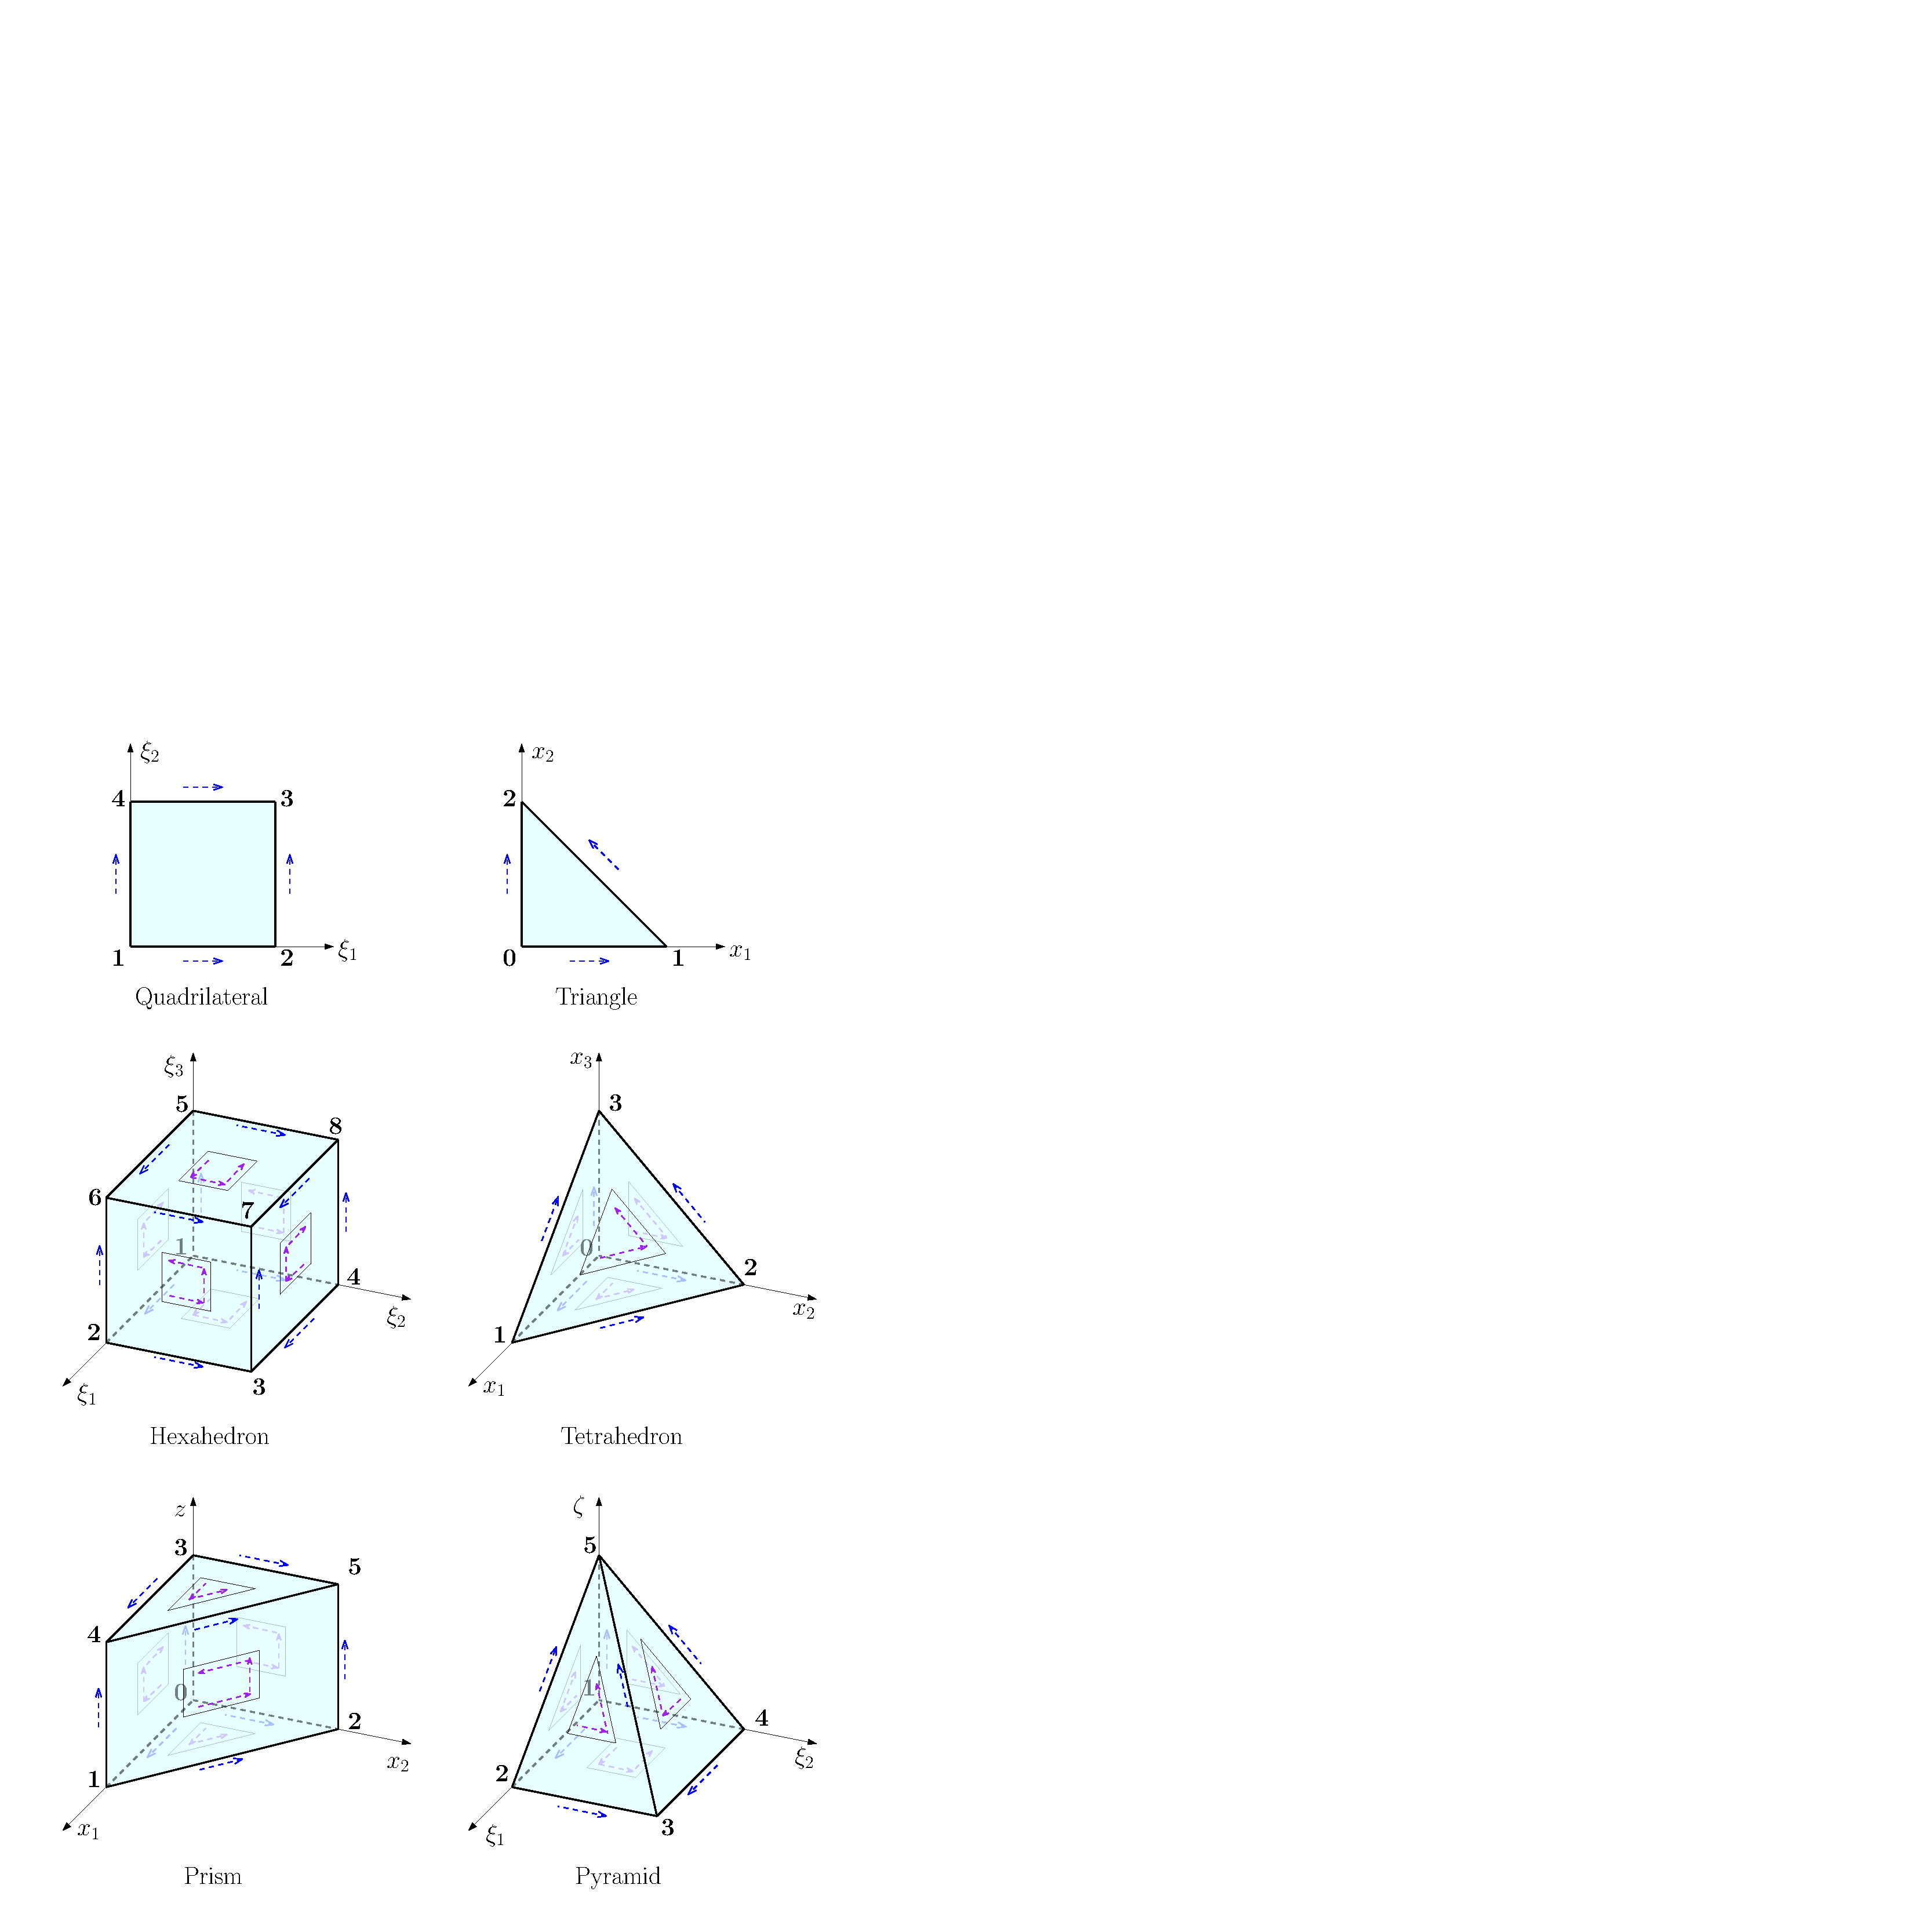
\includegraphics[scale=0.5]{./figures/LocalOrientationsTables.pdf}
	\end{center}
\end{minipage}} &\\[-10pt]
\multicolumn{3}{|c|}{} &\\[-17pt]
{}& {} &{} &\\[-5pt]
\multicolumn{3}{r}{\footnotesize\textit{continued on next page}} &\\[-18.5pt]
\hline
\end{tabular}
\end{center}
\renewcommand{\arraystretch}{1}%Back to normal spacing

\newpage

%%%%%%%%%%%%%%%%%%%%%Orientations 2: Permutations%%%%%%%%%%%%%%%%%%%%%
\renewcommand{\arraystretch}{1.35}%Better row spacing
\begin{center}
\begin{tabular}
{|C{0.35cm} L{11.9cm} C{2.9cm}|N}%See main file for this custom columns - they keep a fixed width while maintaining aligment
\multicolumn{3}{l}{\footnotesize\textit{continued from previous page}} &\\[-2pt]
\hline
\multicolumn{3}{|c|}{\large \textbf{Orientations}} &\\
\hline
\multicolumn{3}{|c|}{Local-to-Global Permutation Functions} &\\
\hline
{}& {} &{} &\\[-15pt]%To keep total width fixed
\multicolumn{3}{|l|}{Edge} &\\
\multicolumn{3}{|l|}{
$	\begin{gathered}
		\quad\quad\quad\!\!\!\sigma_\oo^\E(s_0,s_1)=\begin{cases}\sigma_0^\E(s_0,s_1)=(s_0,s_1)&\quad\text{if  }\,\oo=0\\
			\sigma_1^\E(s_0,s_1)=(s_1,s_0)&\quad\text{if  }\,\oo=1\end{cases}
	\end{gathered}$} &\\
\multicolumn{3}{|l|}{Quadrilateral Face} &\\
\multicolumn{3}{|l|}{
$	\begin{gathered}
			\sigma_\oo^\square(s_0,s_1,t_0,t_1)=\begin{cases}
		\sigma_0^\square(s_0,s_1,t_0,t_1)=(s_0,s_1,t_0,t_1)&\quad\text{if  }\,\oo=0\\
		\sigma_1^\square(s_0,s_1,t_0,t_1)=(t_0,t_1,s_1,s_0)&\quad\text{if  }\,\oo=1\\
		\sigma_2^\square(s_0,s_1,t_0,t_1)=(s_1,s_0,t_1,t_0)&\quad\text{if  }\,\oo=2\\
		\sigma_3^\square(s_0,s_1,t_0,t_1)=(t_1,t_0,s_0,s_1)&\quad\text{if  }\,\oo=3\\
		\sigma_4^\square(s_0,s_1,t_0,t_1)=(t_0,t_1,s_0,s_1)&\quad\text{if  }\,\oo=4\\
		\sigma_5^\square(s_0,s_1,t_0,t_1)=(s_1,s_0,t_0,t_1)&\quad\text{if  }\,\oo=5\\
		\sigma_6^\square(s_0,s_1,t_0,t_1)=(t_1,t_0,s_1,s_0)&\quad\text{if  }\,\oo=6\\
		\sigma_7^\square(s_0,s_1,t_0,t_1)=(s_0,s_1,t_1,t_0)&\quad\text{if  }\,\oo=7\end{cases}
	\end{gathered}$} &\\
\multicolumn{3}{|l|}{Triangle Face} &\\
\multicolumn{3}{|l|}{
$	\begin{gathered}
	\quad\sigma_\oo^\Tri(s_0,s_1,s_2)=\begin{cases}
		\sigma_0^\Tri(s_0,s_1,s_2)=(s_0,s_1,s_2)&\quad\text{if  }\,\oo=0\\
		\sigma_1^\Tri(s_0,s_1,s_2)=(s_1,s_2,s_0)&\quad\text{if  }\,\oo=1\\
		\sigma_2^\Tri(s_0,s_1,s_2)=(s_2,s_0,s_1)&\quad\text{if  }\,\oo=2\\
		\sigma_3^\Tri(s_0,s_1,s_2)=(s_0,s_2,s_1)&\quad\text{if  }\,\oo=3\\
		\sigma_4^\Tri(s_0,s_1,s_2)=(s_1,s_0,s_2)&\quad\text{if  }\,\oo=4\\
		\sigma_5^\Tri(s_0,s_1,s_2)=(s_2,s_1,s_0)&\quad\text{if  }\,\oo=5\end{cases}
	\end{gathered}$} &\\
\multicolumn{3}{|c|}{} &\\
\multicolumn{3}{|c|}{\small\fbox{\parbox[c][40pt][c]{0.75\textwidth}{In the expressions for the shape functions, precompose the ancillary operators (and their differential form) with the corresponding permutation function to obtain orientation embedded shape functions.}}} &\\
\multicolumn{3}{|c|}{} &\\[-23pt]
{}& {} &{} &\\
\hline
\end{tabular}
\end{center}
\renewcommand{\arraystretch}{1}%Back to normal spacing